\documentclass{report}
\usepackage[style=ieee,backend=bibtex]{biblatex} 
\usepackage{amsmath,amsfonts}
\usepackage{geometry}
\usepackage{bm}
\usepackage{bytefield}
\usepackage{listings}
\usepackage{longtable} % for 'longtable' environment
\usepackage{pdflscape} % for 'landscape' environment
\usepackage{rotating}
\usepackage{tabularx}
\usepackage{multirow}
\usepackage[binary-units,separate-uncertainty=true]{siunitx}
\usepackage{pgfgantt}
\usepackage{float}
\usepackage{svg}
\usepackage{subcaption}
\usepackage{hyperref}
\usepackage[version=4]{mhchem}
\usepackage[useregional]{datetime2}

\bibliography{main.bib,websites.bib,datasheets.bib} 

% Declare custom (Non-si) units
\DeclareSIUnit\feet{ft} % Yes I know feet aren't SI unit...
\DeclareSIUnit\year{y}
\DeclareSIUnit\gacc{\textit{g}}
\DeclareSIUnit\siaxis{\text{axis}}
\DeclareSIUnit\baud{bd}
\DeclareSIUnit\mmDA{mm\, DA}
\DeclareSIUnit\octave{oct}

% https://tex.stackexchange.com/a/121871
\newcommand*{\secref}[1]{section \hyperref[{#1}]{\ref*{#1} \nameref*{#1}}}
\newcommand*{\Secref}[1]{Section \hyperref[{#1}]{\ref*{#1} \nameref*{#1}}}

% https://tex.stackexchange.com/a/12712
\newcolumntype{L}[1]{>{\raggedright\let\newline\\\arraybackslash\hspace{0pt}}m{#1}}
\newcolumntype{C}[1]{>{\centering\let\newline\\\arraybackslash\hspace{0pt}}m{#1}}
\newcolumntype{R}[1]{>{\raggedleft\let\newline\\\arraybackslash\hspace{0pt}}m{#1}}

% https://tex.stackexchange.com/a/24133
\newcommand{\textoverline}[1]{$\overline{\mbox{#1}}$}

\newcommand{\hlreq}[1]{\hyperlink{req-#1}{\textbf{#1}}}

\newcommand{\liion}{\ce{Li}-ion}
\newcommand{\aud}{A\$}
\newcommand{\ssh}{\texttt{ssh}}
\newcommand{\iic}{{I\textsuperscript{2}C}}

\ganttset{calendar week text={\small{\startday/\startmonth}}}

\begin{document}

\begin{titlepage}

  % Center the content
  \begin{center}

    % Title
    % \vspace*{3cm}
    {\LARGE\bfseries Design of an Experiment to Evaluate High-Power Rockets as a CubeSat Qualification Platform} \\[3cm]



    % Author's name
    {\Large Author: Peter Tanner} \\[1cm]

    % Supervisor's name
    {\Large Supervisor: Dilusha Silva} \\[2cm] % \\[3cm]

    % Degree text
    {\large ATTENTION: THIS IS A DRAFT VERSION. TODO: CHECK CHECKLIST BEFORE SUBMITTING }
    {\large \textit{This thesis is presented in partial fulfilment of the requirements for the degree of Bachelor of Philosophy
      (Honours) at the University of Western Australia}} \\[1cm]

    % Faculty information
    {\large Faculty of Engineering and Mathematical Sciences} \\[3cm]

    {\large Word count: TODO:} \\
    {\large Submitted: \today} \\[2cm]

    \includesvg[width=0.495\textwidth]{images/UWA-logo-dark.svg} \\

  \end{center}

\end{titlepage}

% LTeX: enabled=false 
% TODOLIST
%TC:igDnore
\newpage
\section{TODO: (!! REMOVE BEFORE FINAL RELEASE !!)}
\begin{itemize}
  \item \texttt{[ ]} Add schematics and PCB gerbers to appendix using \texttt{pdfpages}
  \item \texttt{[ ]} Add links to source repository \url{https://git.petertanner.dev/hpr-evaluation/}
  \item \texttt{[ ]} Use \LaTeX template for Honours papers
  \item \texttt{[ ]} Resolve all warnings except badness warnings because I don't know how to control that
  \item \texttt{[ ]} Make BibTeX consistent
  \item \texttt{[ ]} Bad citation format for datasheets and websites (Date is after access date).
  \item \texttt{[ ]} Check grammar and spelling
  \item \texttt{[ ]} Check presentation/typesetting
  \item \texttt{[ ]} Resolve all \texttt{TODO:} comments
  \item \texttt{[ ]} ADD ENGINEERING COVERSHEET WITH HONORS DECLARATION.
  \item \texttt{[ ]} Finish all items on this checklist
\end{itemize}


\paragraph{Wts}
\begin{itemize}
  \item PROJECT BODY (ASSUME EXPERIMENTAL PROJECT)
        \subitem 20\% INTRODUCTION AND LITERATURE REVIEW
        \subitem 15\% EXPERIMENTAL DESIGN
        \subitem 35\% RESULTS AND DISCUSSION
  \item 10\% CONCLUSION AND FUTURE WORK
  \item 10\% SCOPE
  \item 10\% PRESENTATION (SHOULD BE GUARANTEED...)
\end{itemize}

\paragraph{USING FORMULA \texttt{WC * SECTION/80\%}}
\begin{itemize}
  \item INTRODUCTION AND LITERATURE REVIEW: 3000 TO 4500 WORDS
  \item EXPERIMENTAL DESIGN: 2250 TO 3375
  \item RESULTS AND DISCUSSION: 5250 TO 7875
  \item CONCLUSION AND FUTURE WORK: 1500 TO 2250
\end{itemize}


%TC:endignore
% END TODOLIST
% LTeX: enabled=true 

\newpage

% TODO: SCOPE
\section*{Abstract}

The CubeSat is a type of small satellite created to reduce the cost of access to space for universities due to its standardised $\SI{10x10x10}{\centi\metre}$ form factor. The total number of CubeSats launched into space is growing exponentially due to their low cost, doubling every $\SI{2.5}{\year}$, however the mission success rate has stalled at 75\% since 2018 \cite{welle2020overview,bouwmeester2022improving}.

Vibration and shock tests are qualification procedures which aim to emulate launch conditions, however they cannot perfectly replicate them \cite{gordon2015benefits}. Testing of CubeSats on suborbital high-power rockets (HPR) is a novel qualification method that can potentially better replicate launch conditions compared to a shaker table, and therefore better detect issues and improve the likelihood of mission success. While there have been tests of university CubeSats on HPRs \cite{slongo2019pre}, there are no direct comparisons to shaker tables to evaluate their effectiveness for qualification.

This paper outlines the design of a data acquisition system (DAQ) to measure vibration from the HPR launch and shaker table tests and finally makes a direct comparison of the vibration environment on the HPR launch and vibration table.


\section*{Acknowledgements}

I'd like to thank all the people and organisations who have supported me throughout this project. Dilusha Silva for being a wonderful mentor and for coordinating the project. Michal Zawierta for his expertise flying drones for the drone tests of the CubeSat. Jamir Khan for being a wonderful friend and engineer who worked on the mechanical side of this project, including construction of the high-power rocket, and for putting up with all my delays. Timothy Ludovico for designing the camera payload and being all around wonderful to work with. Jeremy Marelich and AVI for providing their shaker table facilities and conducting the tests. UWA Aerospace for being a wonderful institution who has been with me from first year through my growth as an engineer and has supported me through this project. Space Angel for creating this project and providing expertise and connections to the Indian Institute of Space Science and Technology (IIST). Dr. Priyadarshnam Hari and the Indian Institute of Space Science and Technology for providing their launch expertise and opportunity to launch on POEM. International Space Centre for supporting this project with funding.

% TODO: ACKNOWLEDGE ALTIUM DESIGNER?

\newpage
\tableofcontents
\newpage

\renewcommand{\listfigurename}{
  \section*{List of Figures}
}
\listoffigures
\cleardoublepage
\renewcommand{\listtablename}{
  \section*{List of Tables}
}
% \renewcommand{\chaptername}{Part}
\listoftables
\cleardoublepage

\chapter{Introduction}
\section{Background}
% Introduction or Background This provides the reader with the context of the project. For example, what is the application area, why is it important, what (in general terms) has been done before?

The University of Western Australia (UWA) Microelectronics Research Group (MRG) is developing a 2U CubeSat to measure the health of vegetation through an infrared camera array \cite{ludovico2024}. The CubeSat is a type of small satellite created to reduce the cost of access to space for universities due to its standardised $\SI{10x10x10}{\centi\metre}$ form factor. This CubeSat will launch on an Indian Polar Satellite Launch Vehicle (PSLV) in the PSLV Orbital Experiment module (POEM), which will host multiple CubeSats in orbit and will provide services including power and communications to the CubeSat.

The total number of CubeSats launched into space is growing exponentially due to their low cost, doubling every $\SI{2.5}{\year}$, however the mission success rate has stalled at 75\% since 2018 \cite{welle2020overview,bouwmeester2022improving}, which implies a need for novel qualification methods. For most single-launch satellites, increased testing is the optimal strategy to minimise failure \cite{bouwmeester2022improving}. Qualification of the CubeSat is required by the launch provider to minimise the risk of damage to the launch vehicle or other payloads from mission failure. The MRG is planning to qualify this CubeSat on a suborbital high-power rocket (HPR) in combination with traditional vibration and shock tests on a single degree of freedom (SDOF) electrodynamic shaker table.

Vibration and shock testing are typical tests for CubeSats which are intended to replicate the conditions of launch \cite{welle2020overview}. Despite their widespread use, SDOF vibration and shock tests do not perfectly replicate the conditions at launch as \cite{gordon2015benefits,nath2022study}:
\begin{enumerate}
  \item The peak flight responses are not able to be achieved since a vibration table cannot simulate steady-state thrust forces since they only can simulate dynamic forces \cite{gordon2015benefits}.
  \item A SDOF test can only excite one axis at a time which is not representative of the launch environment \cite{gordon2015benefits,nath2022study}.
  \item A vibration table tests a "fixed-base" case which has different modes compared to the case where the satellite is fixed to the launch vehicle \cite{gordon2015benefits}.
\end{enumerate}

A HPR has a higher total impulse than model rockets but a lower impulse than sounding rockets, with a range of \SI{36}{\newton\second} up to \SI{163840}{\newton\second}, and have a sub-orbital trajectory unlike launch vehicles \cite{pierce2019development}. Suborbital rockets have been used for testing several CubeSats \cite{9316404,minelli2019mobile}, however this qualification method is not in widespread use in the industry.

\section{Problem Identification}
% Problem Identification What is the problem that you are trying to solve, or the hypothesis that you are intending to test? What is your intended contribution to the state of the art?
For institutions with limited budget, shock and random vibration tests using a SDOF vibration table is the current state of the art (SOTA) method for qualification. HPRs are a potential qualification method which can complement SDOF vibration tests, however there is no prior studies comparing both HPRs and SDOF vibration tests against the qualification level set by the launch provider. If HPRs can produce a vibration environment similar to the qualification level, HPRs may be a useful complement to SDOF vibration tests and may increase success rates.

Since HPRs are not frequently used, another issue is the lack of tooling for making HPRs an effective test platform. This research will involve design and evaluation of a combined test and data acquisition platform which:
\begin{enumerate}
  \item Measures the vibration response of the rocket on the CubeSat required for evaluating the HPR platform and
  \item Emulates the POEM satellite bus services to ensure the payload-under-test has access to the same environment as on launch.
\end{enumerate}

An experiment will be designed using the DAQ data to evaluate HPRs.

\chapter{Literature Review}
% Literature Review or Previous Work Explain the literature (e.g. refereed research papers) or previous body of work (e.g. previous projects within the research group) on which your investigation is based. This should not simply be a linear account, but rather a synthesis of what is important from what has gone before. It will often be a hierarchical account, moving from a general understanding of the field, to identification and expansion of work that is specifically relevant to your project

This literature review will cover the current testing methods used in CubeSats, the use of suborbital rockets as a qualification method and cover the types of sensors and systems required to record these tests.

\section{Standard Satellite Qualification Methods}
There are multiple satellite qualification standards, an example is the NASA General Environmental Verification Specification (GEVS) which is a panel of tests including electromagnetic compatibility (EMC), thermal, acoustic and vibration tests that are required for all NASA Goddard Space Flight Center projects \cite{nasa-gevs}. Other standards include ISO-15864, JERG-2-002, NASA-STD-7002A, ECSS-E-ST-10-03C and SMC-S-01 \cite{cho2012overview}. While these standards have flight heritage, being used on many successful payloads, they were designed for medium or large satellites, and therefore fully complying with these standards are out of the budget of most university CubeSat programs \cite{cho2012overview}. While is no widely used test standard for CubeSats currently in use, since most CubeSat projects are budget constrained, there is a de facto minimum series of tests which are random vibration, shock and thermal vacuum testing \cite{welle2020overview}.


\subsection{Vibration}
Vibrations are experienced by satellites during transportation and loading, and most prominently during launch \cite{brown_elements_2002}. The purpose of vibration testing is to ensure that the satellite will survive transportation and launch conditions, and to find workmanship errors \cite{brown_elements_2002,gordon2015benefits}.

\subsubsection{Random Vibration Test}
In the random vibration test, a vibration profile is applied to the satellite which tests all the resonant frequencies of the satellite \cite{nieto2019cubesat}. This range includes frequencies on the order of $\SIrange{100}{1000}{\hertz}$, since higher frequencies couple to the satellite through acoustic means rather than through the structure \cite{gordon2015benefits}. An example of a random vibration profile and its response is shown in figure \ref{fig:random}. A sine sweep vibration test is similar, but instead of the frequency being randomly sampled it is swept through sequentially from either low to high frequency or vice versa.

\begin{figure}[H]
  \centering
  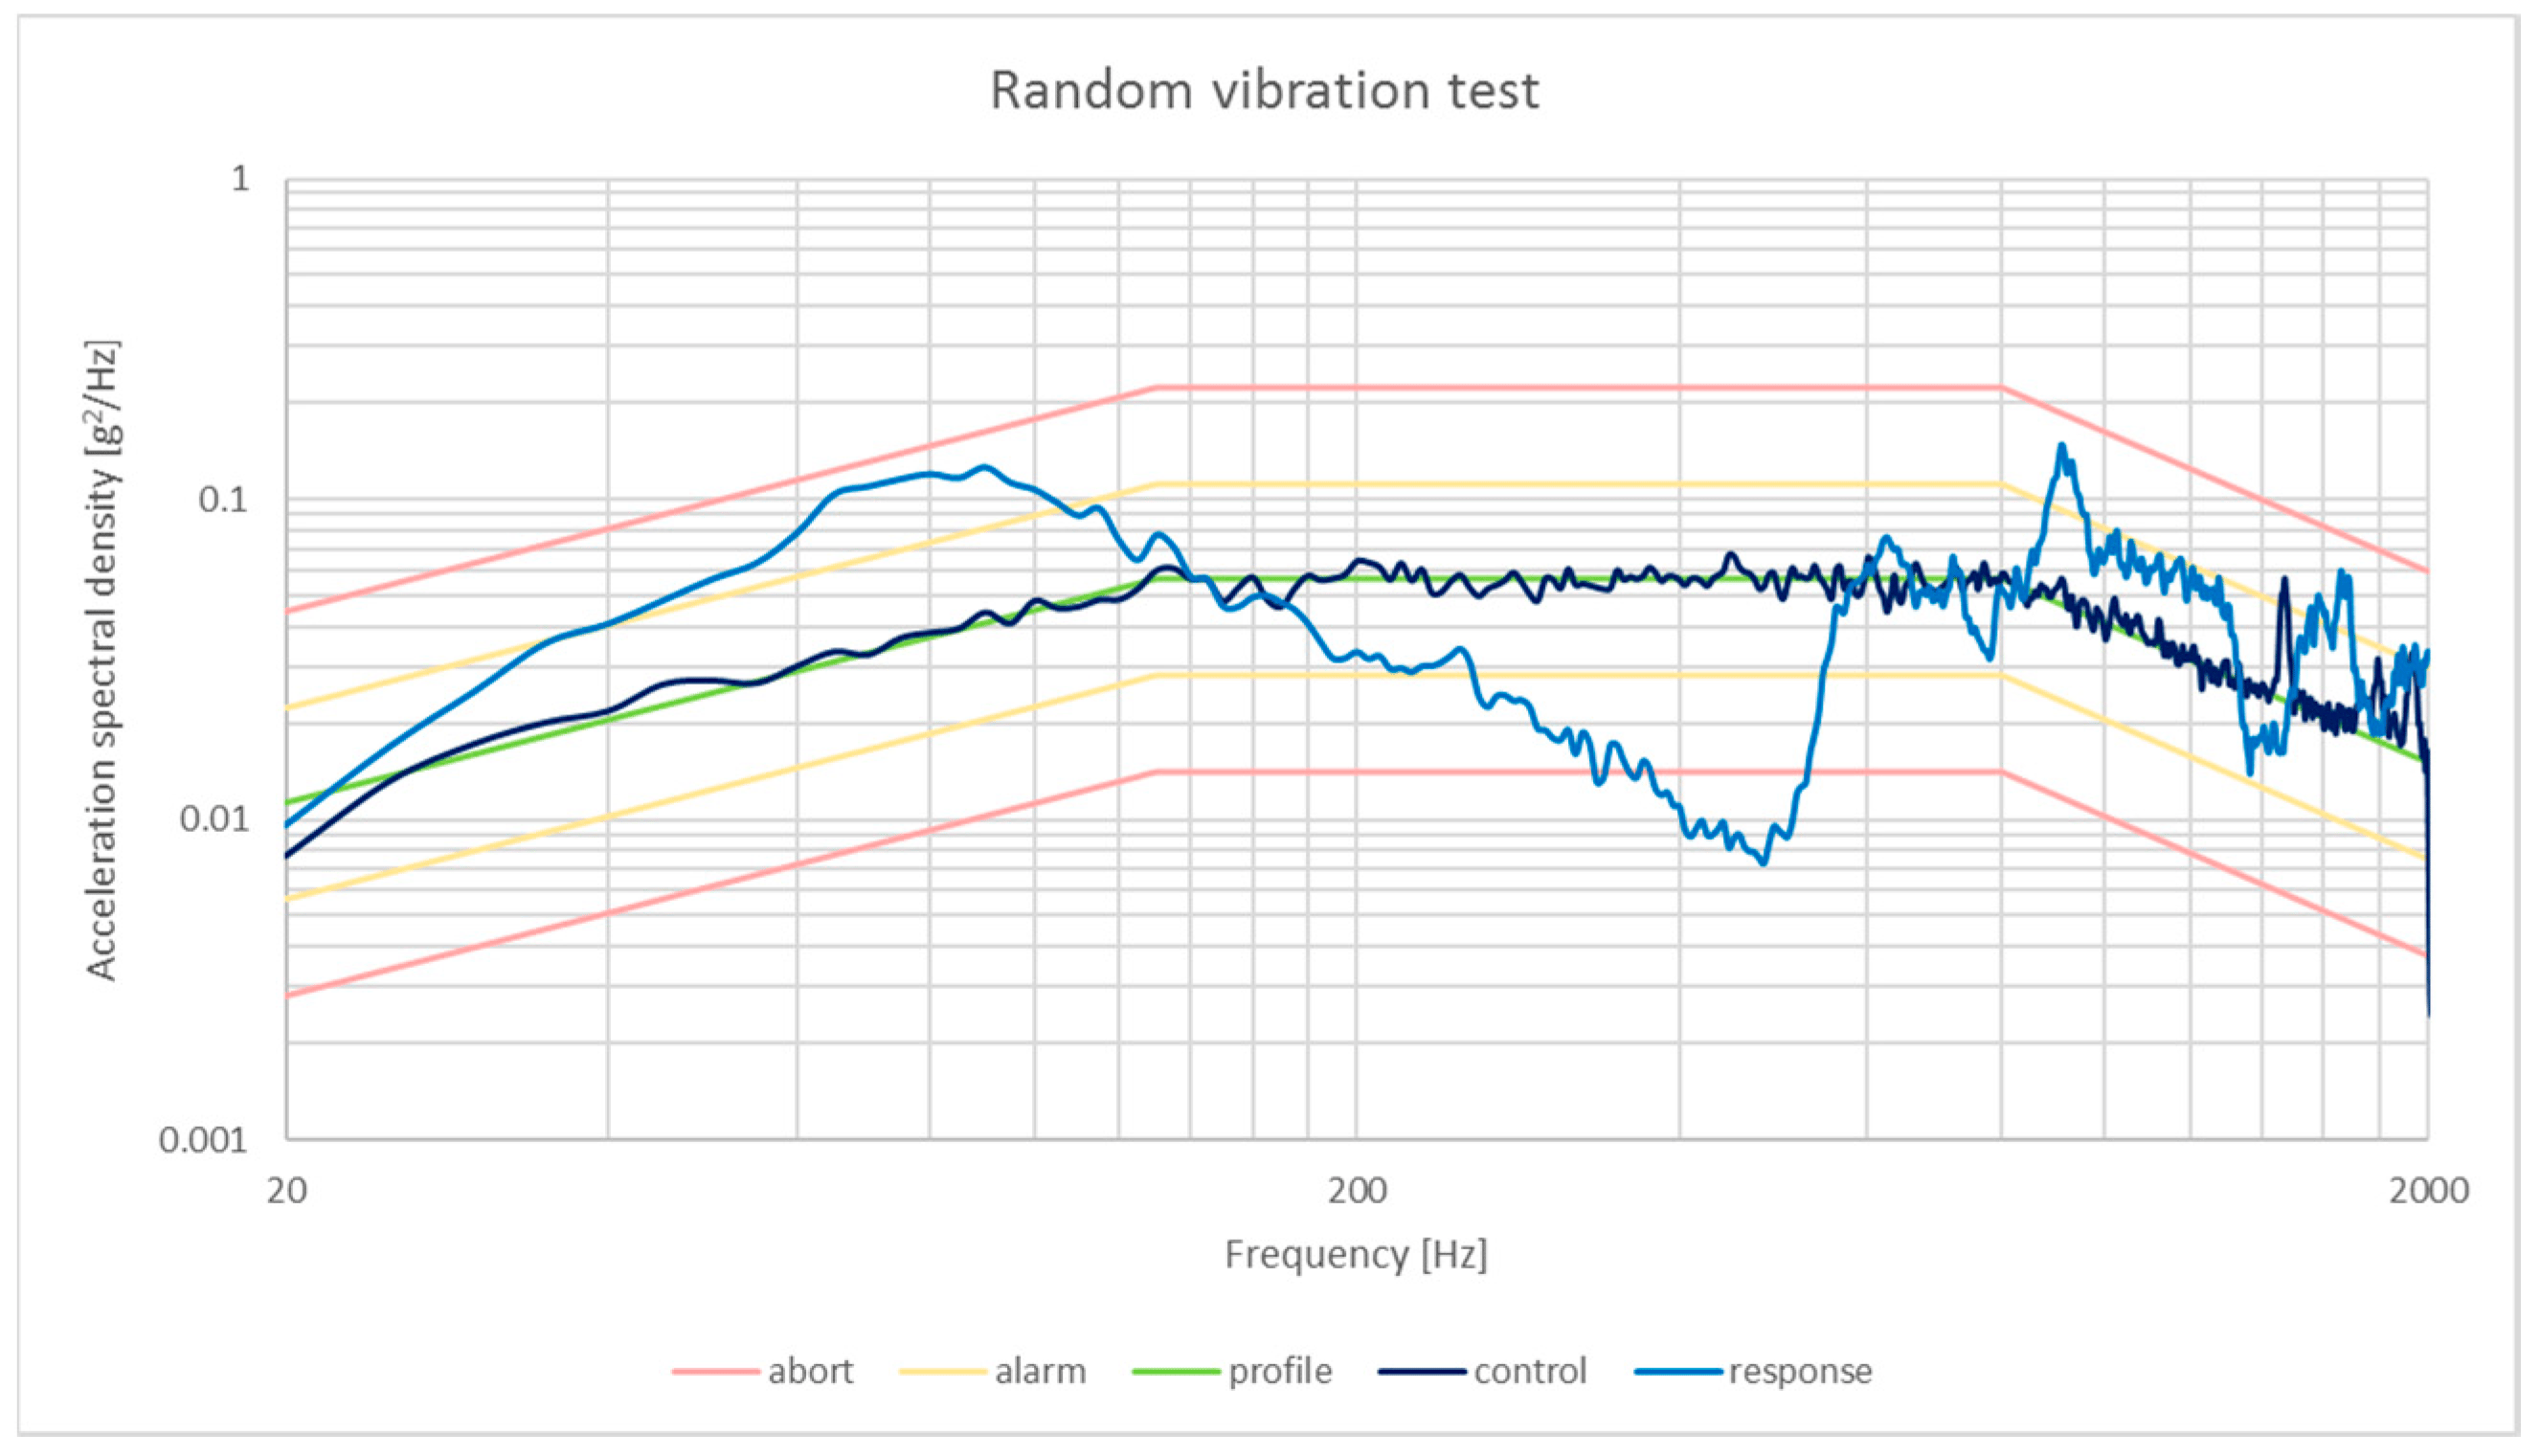
\includegraphics[width=0.75\textwidth]{images/random-study.png}
  \caption{Random vibration test \cite{nieto2019cubesat}}
  \label{fig:random}
\end{figure}

The limitations of random vibration tests is that the shaker and table will have different modes than the launch vehicle and payload mount, resulting in the test response not perfectly matching the flight response \cite{gordon2015benefits,aglietti2019spacecraft}. Gordon and Kern argue that this difference is not a factor in practice since shaker tests are "not intended to be a strength test"  \cite[p.~7]{gordon2015benefits} and that components "should have been strength qualified prior to integration" \cite[p.~7]{gordon2015benefits}. Component level is argued as a best practice in the CubeSat community \cite{rawsonbest}, however some argue that component level testing is not suited to the short timeline of university CubeSat projects and that more effort should be put into integration testing \cite{decker2016systems}. If a testing program focuses on integration testing, then this mismatch between shaker table and flight response could result in the CubeSat not being properly qualified.

While 6 degrees of freedom (DOF) shaker tables exist which can replicate the vibrations experienced in all dimensions during launch, most satellites are still tested with single-axis shaker tables \cite{gordon2015benefits,aglietti2019spacecraft,nath2022study}. While Gordon and Kern \cite{gordon2015benefits} state that these limitations are adequately managed by testing in all three orthogonal axes separately, Aglietti and Nath \cite{nath2022study} created a model of three, two and single axis vibration tests and found that to match the 3 DOF response with a single DOF table, the satellite needed to be subjected to 2.5 times the $g_\text{rms}$ forces than in 3 DOF testing, leading to the satellite being over designed \cite{nath2022study}.

\subsubsection{Quasi-Static Acceleration Test (QAT)}
A quasi-static test simulates liftoff, where there is a combination of random vibration from engines and quasi-static acceleration from the engine and other external forces on the launch vehicle \cite{nieto2019cubesat,brown_elements_2002}, which are approximated as constant forces at selected frequencies as shown in figure \ref{fig:qatforces}. The QAT is usually compared to results from coupled loads analysis, where all forces are assumed to be applied to the satellite through the launch vehicle as shown in figure \ref{fig:cla} \cite{dickens2001coupled}.

\begin{figure}[H]
  \centering
  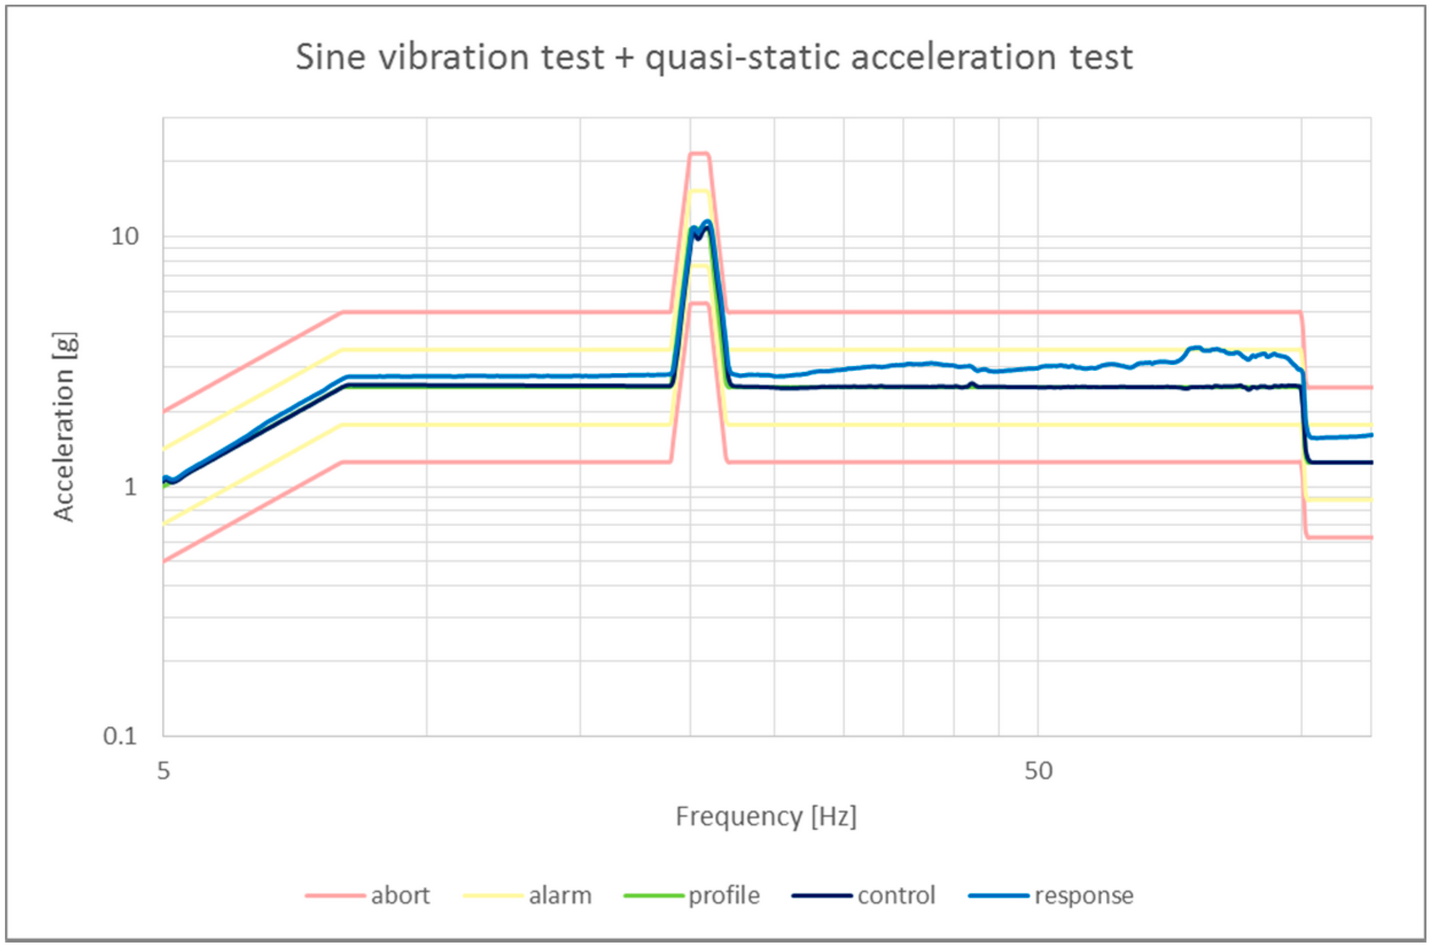
\includegraphics[width=0.75\textwidth]{images/qat.png}
  \caption{Quasi-static acceleration test. The input profile high acceleration from $\SI{20}{\hertz}$ to $\SI{21}{\hertz}$, resulting in the response having a force of 10.8 \textit{g} acceleration around this frequency \cite{nieto2019cubesat}}
  \label{fig:qatforces}
\end{figure}

\begin{figure}[H]
  \centering
  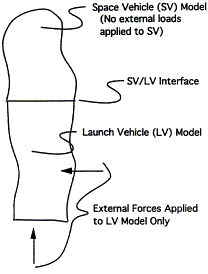
\includegraphics[width=0.3\textwidth]{images/cla.png}
  \caption{Coupled loads model \cite{dickens2001coupled}}
  \label{fig:cla}
\end{figure}

The first limitation of a quasi-static acceleration test is that the shaker table cannot apply the peak response evenly that is predicted by coupled loads analysis (CLA) \cite{gordon2015benefits}. Again, Gordon and Kern state that these limitations are addressed by component-level strength qualification. They also state that applying the peak response evenly is not necessary, since if an item does not fail, the correctly applying the response evenly does not greatly increase its likelihood of failing \cite{gordon2015benefits}. The second limitation is there is a difference in modes, since a quasi-static acceleration test also contains random vibrations \cite{gordon2015benefits}.

\subsection{Shock}

Shock is experienced by satellites when pyrotechnics are detonated or deflagrated during events such as staging and ignition, the response appears as a range of decaying sinusoids in the $\SI{100}{\hertz}$ to $\SI{10}{\kilo\hertz}$ frequency range \cite{brown_elements_2002}, which decay in $\SI{5}{\milli\second}$ to $\SI{15}{\milli\second}$ \cite{brown_elements_2002}. The spectrum extends up to $\SI{40}{\kilo\hertz}$, however for analysis frequencies above $\SI{10}{\kilo\hertz}$ are assumed to be non-damaging \cite{bement1995manual,nasa-pyroshock}. Pyroshock may cause peak accelerations of up to 10000 \textit{g} \cite{nasa-pyroshock}. High explosives are primarily used for explosive elements on rockets in combination with some low explosives for initiators \cite{bement1995manual}.

Shock is tested using a shock-generating device which is applied to the satellite along all three axes \cite{nasa-gevs,nasa-pyroshock}, the shock generating device for a CubeSat can be an electrodynamic shaker table \cite{nieto2019cubesat} with a half-sine profile \cite{nieto2019cubesat}. The shock test has similar limitations as the random vibration test, since it also uses a shaker table to affect the satellite.

Shock are simulated to create a shock response spectrum (SRS), which plots the maximum acceleration per frequency bin. The SRS contains an octave slope which rises to the first resonant frequency called the "knee frequency". The octave slope can be approximately \SI{9}{\decibel\per\octave} to \SI{12}{\decibel\per\octave} depending on distance to the source.

\begin{figure}[H]
  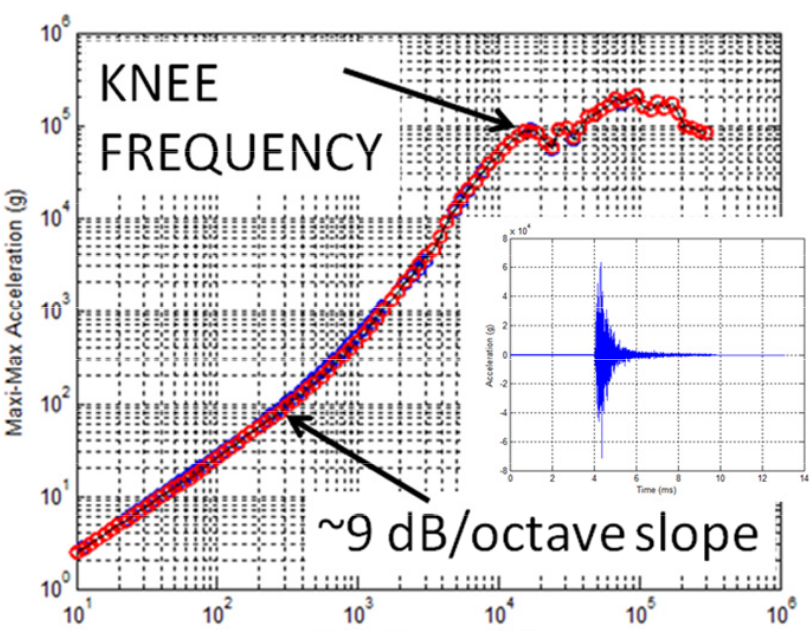
\includegraphics[width=0.495\textwidth]{images/pyroshock2.png}
  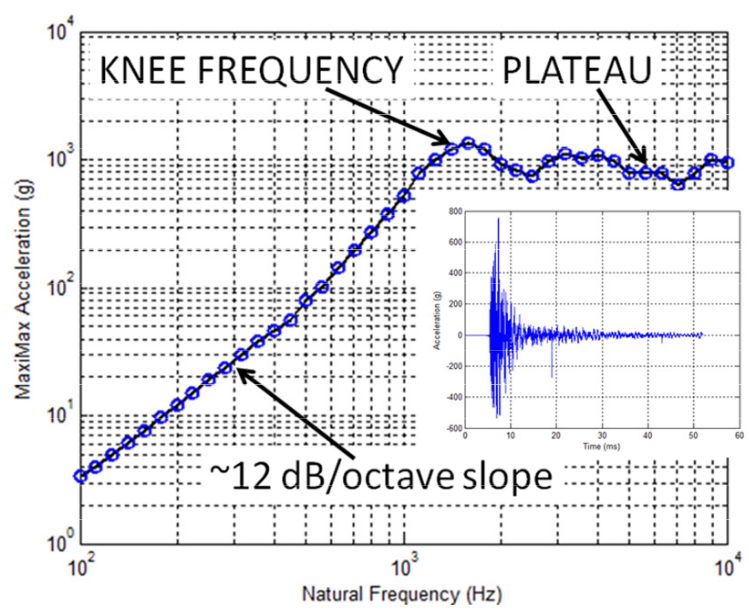
\includegraphics[width=0.495\textwidth]{images/pyroshock1.png}
  \caption{Shock response spectrum of and time-domain shock response. Left: near-field (close to shock source). Right: far-field (distant from shock source) \cite{nasa-pyroshock}}
  \label{fig:pyroshock}
\end{figure}

\subsection{Functional testing}

The CubeSat's functionality is typically tested using "day-in-the-life" testing where a 24-hour period of the CubeSat's on-orbit life is tested on the ground \cite{venturini2018improving}. Simulating the on-orbit conditions is an important factor in this test, for example GPS and star field simulators are commonly used \cite{venturini2018improving}.

Doyle et al. propose an extension to day-in-the-life testing called mission testing which involves simulating the long term CubeSat mission on the ground instead of one 24-hour cycle \cite{doyle2021mission}. This requires accurately simulating the on-orbit conditions of the CubeSat for an extended and uninterrupted period of time (several weeks), and must also simulate nominal and emergency events that may be encountered in orbit \cite{doyle2021mission}.

On-orbit conditions that may be simulated include interacting with the CubeSat only through its radio and providing the same amount of power that would be seen in orbit.

\section{Rocket Testing of CubeSats}
\subsection{Sounding Rockets}
Sounding rockets are a class of suborbital rocket used between $\SI{40}{\kilo\metre}$ and $\SI{200}{\kilo\metre}$, above where weather balloons operate \cite{seibert2006history}. While sounding rockets have been used to launch many CubeSats with suborbital trajectories, such as in the REXUS-25 mission \cite{pont2019rexus}, there has been only one instance of sounding rockets being used as an additional qualification platform for a CubeSat \cite{slongo2019pre}. The FloripaSat-I CubeSat was tested on a VSB-30 sounding rocket \cite{slongo2019pre} to qualify the CubeSat under launch conditions. This qualification method was intended not to replace, but to complement standard vibration and shock qualification methods \cite{slongo2019pre}. The test measured these launch conditions through the micro-electromechanical systems (MEMS) based MPU6050 inertial measurement unit (IMU) \cite{slongo2019pre}.

\begin{figure}[H]
  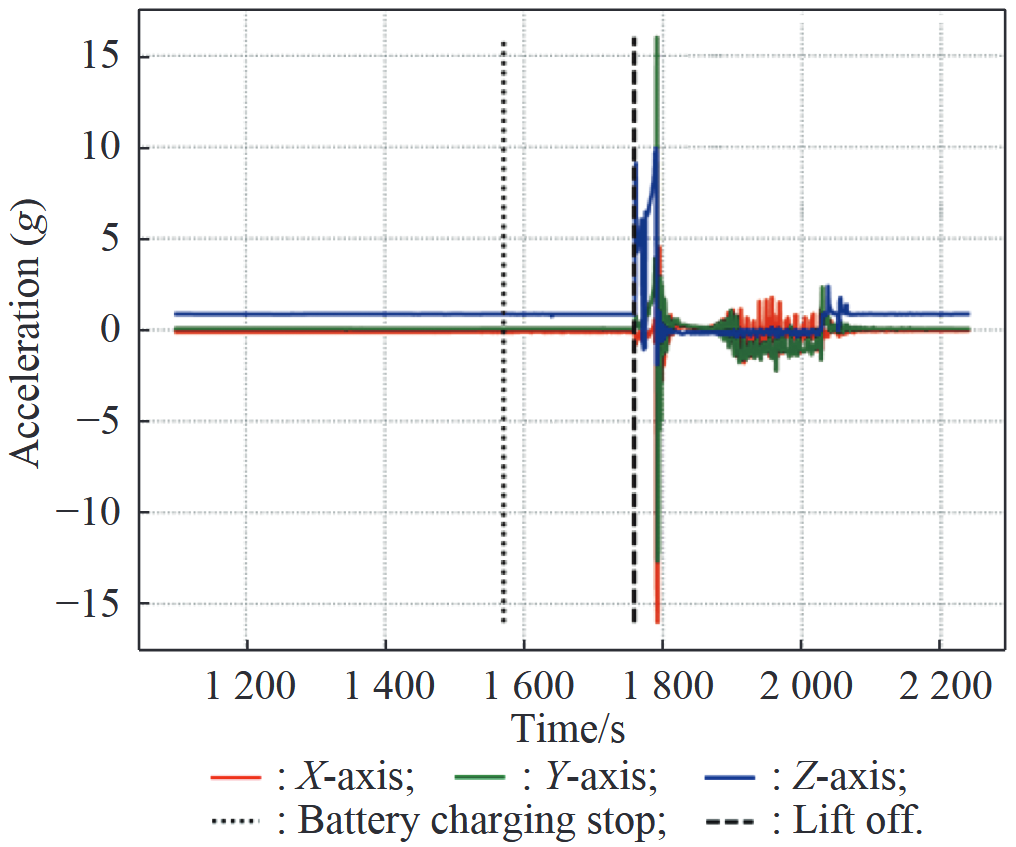
\includegraphics[width=0.495\textwidth]{images/floripa-accel.png}
  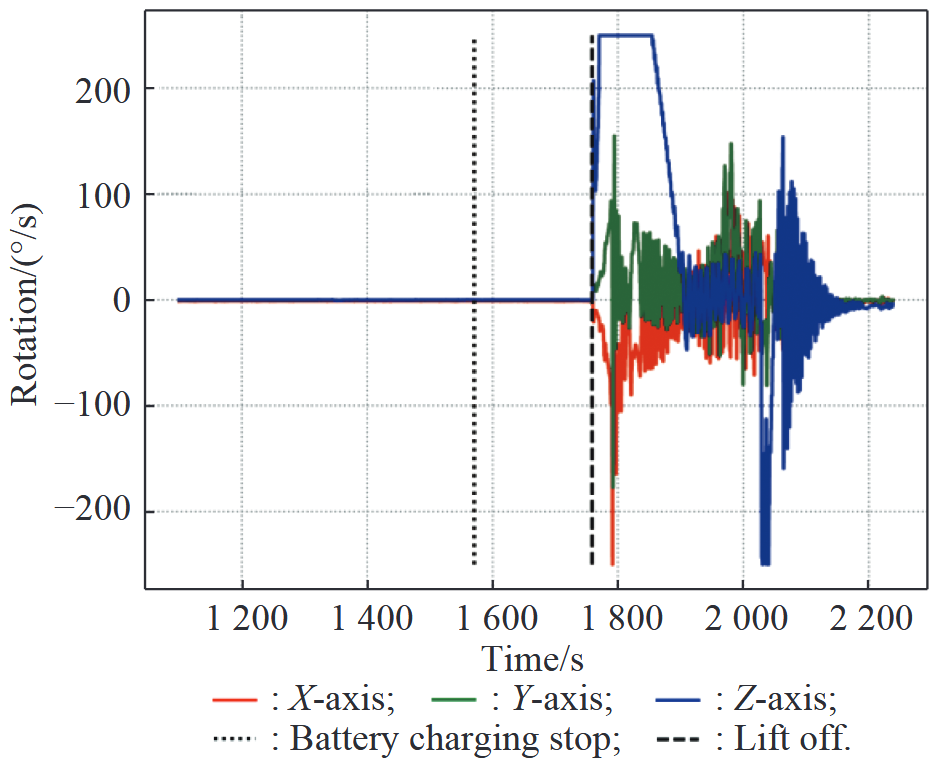
\includegraphics[width=0.495\textwidth]{images/floripa-rot.png}
  \caption{Acceleration in time domain (Left), Angular velocity in time domain (Right) during the launch of FloripaSat-I \cite{9316404}}
  \label{fig:accel-rot}
\end{figure}

While this study does show the time-domain accelerometer and gyroscope measurements from the sounding rocket launch in figure \ref{fig:accel-rot}, it does not compare the data to other qualification tests in the FloripaSat-I campaign, including random vibration and shock testing. Additionally, the launch data was not presented in the frequency domain through the boost and coast phases of the flight, meaning they could not be compared to the acceleration spectra which was shown for the shaker table testing in figure \ref{fig:shaker}.

\begin{figure}[H]
  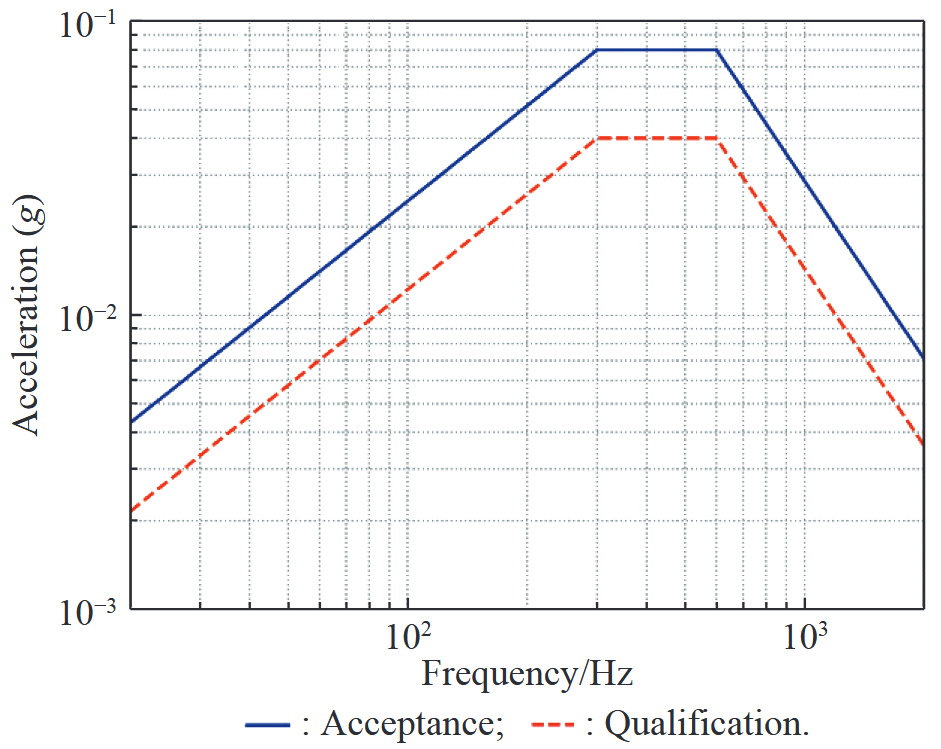
\includegraphics[width=0.495\textwidth]{images/floripa-random-spectrum.png}
  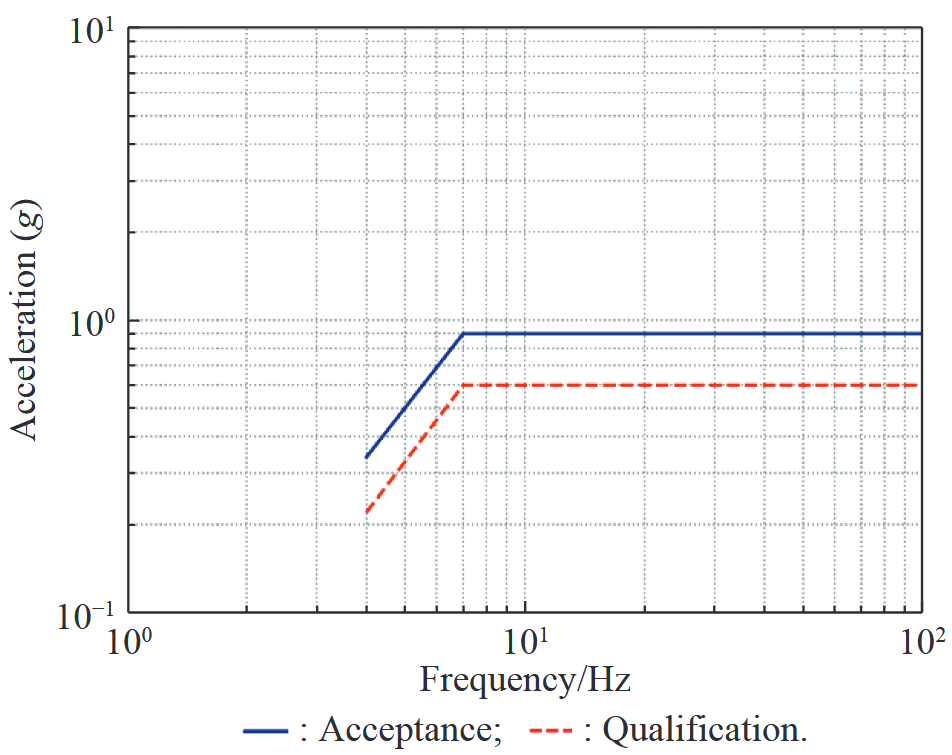
\includegraphics[width=0.495\textwidth]{images/floripa-sinusoid.png}
  \caption{Random vibration (Left) and sine sweep (Right) tests on a shaker table during the qualification of FloripaSat-I \cite{9316404}}
  \label{fig:shaker}
\end{figure}

Another shortcoming of the study is that a shock test using a half-sine pulse was not performed. The use of a sounding rocket is a potential method of qualifying the CubeSat's ability to tolerate shocks since there will be shock events when pyrotechnics are lit to stage the rocket, although the forces will have lower intensity than on a orbital launch vehicle.

\subsection{High-Power Rockets (HPR)}
While sounding rockets have a significantly lower cost compared to an orbital launch vehicle, they cost \$1 million USD per launch to launch $\SI{200}{\kilo\gram}$ on average \cite{jurist2009commercial}, resulting in a specific cost of \$5000 USD/kg, which is still a large amount for university CubeSat programs. High-power rockets (HPR) are a lower-performance but cheaper alternative to sounding rockets, which can leverage the expertise of university rocketry teams while having qualification potential as sounding rockets. A single stage level 3 certification rocket can reach altitudes above $\SI{10000}{\feet}$ \cite{canepa2005modern} for a cost of only \$1200 USD \cite{canepa2005modern}. Despite the potential cost benefits, there have not been any published instances of a HPR being used to qualify a CubeSat.

The typical phases of a HPR launch are \cite{canepa2005modern}:

\begin{itemize} % TODO: FIND SOURCES FOR THIS SECTION
  \item Boost phase: The HPR is being powered by a solid rocket motor. In most HPR launches, this phase only lasts several seconds.
  \item Coast phase: After motor burnout, the rocket follows a ballistic trajectory to its apogee.
  \item Apogee: This is the maximum altitude the rocket will reach. At apogee the drogue parachute is deployed, which limits the rocket's descent velocity.
  \item Main parachute deployment: At a set altitude the main parachute is deployed, which has a higher surface area than the drogue parachute and further slows the rocket to landing velocity. A main parachute should not be deployed at apogee since this results in the rocket drifting further which complicates recovery efforts.
  \item Landing: The rocket lands on the ground and is recovered by the rocketry team for safing (disarming of live energetics) and transportation. While the landing occurs minutes after launch, finding the rocket is a harder task and may occur hours after landing.
\end{itemize}

\begin{figure}[H]
  \centering
  \includesvg[width=0.75\textwidth]{images/rocket_graphic.svg}
  \caption{Typical launch of a single stage high-power rocket}
  \label{fig:rocket_flight}
\end{figure}

One potential issue with HPRs as a qualification platform for shock is that low explosive black powder is used \cite{canepa2005modern} which has different explosive characteristics, such as a subsonic flame front, compared to the high-explosives used in launch vehicles \cite{bement1995manual} and will therefore produce different shock responses. One study \cite{wang2023numerical} performed finite element analysis of igniters filled with low explosives including aluminium potassium perchlorate and boron potassium nitrate and determined the SRS, shown in figure \ref{fig:lowsrs}. Compared to the SRS of high-explosives in figure \ref{fig:pyroshock}, where at a frequency of \SI{1}{\kilo\hertz} the acceleration is over \SI{1000}{\gacc} \cite{nasa-pyroshock}, in these low explosive simulations the acceleration at \SI{1}{\kilo\hertz} is only \SI{10}{\gacc} \cite{wang2023numerical}. Therefore, it is hypothesised that HPRs will not be useful for shock qualification since the response of low explosives is different from the high explosives used on launch vehicles.


\begin{figure}[H]
  \centering
  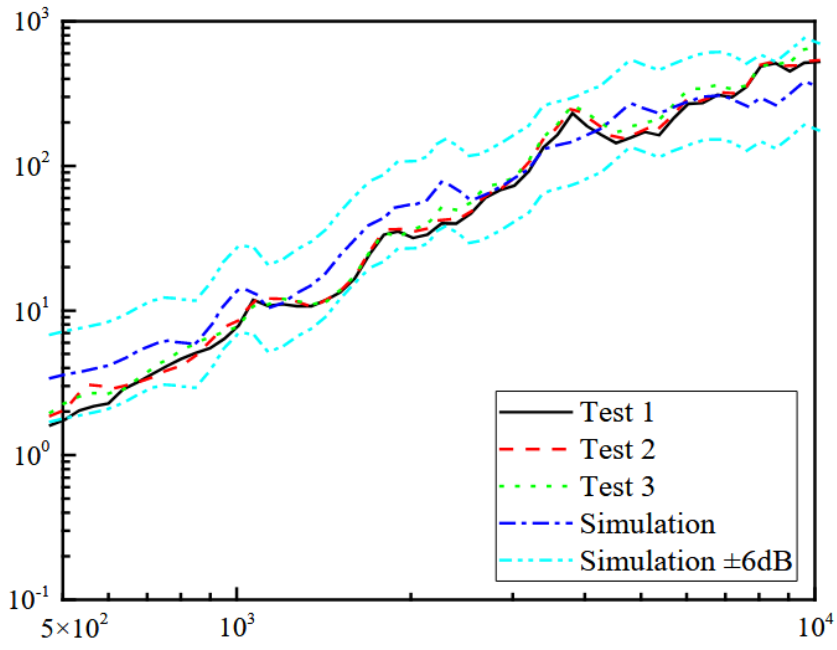
\includegraphics[width=0.75\textwidth]{images/deflagration.png}
  \caption{Shock response spectrum from computer modelling of an igniter based on the low explosive aluminium potassium perchlorate \cite{wang2023numerical}}
  \label{fig:lowsrs}
\end{figure}

\subsection{Avionics Systems}

Some HPR flights use avionics systems which may contain \cite{canepa2005modern,telaak2023designing}:

\begin{itemize}
  \item Radio and GNSS receiver for tracking,
  \item Accelerometer and barometer for measuring acceleration and altitude,
  \item Relays or transistors for firing e-matches to deploy parachutes (known as an electronic deployment).
\end{itemize}

An example of a mature avionics system widely used in HPR is the Telemetrum \cite{telemetrum,telaak2023designing}, which contains a GNSS antenna and receiver, ISM radio, microcontroller, MEMS accelerometer, barometer and pyrotechnic channels \cite{telemetrum}.

Most HPR avionics use MEMS accelerometers, including the MPU6050, MPU9250, ADXL375 and BMX160 \cite{telaak2023designing}. One of the most popular are the MPU6050 \cite{telaak2023designing,moschidis2022arduino}, however this accelerometer is out of production and should not be used in future designs.

\chapter{Design Process}
\label{sec:design-process}

This section outlines in detail the process, shown in figure \ref{fig:design-process-hl}, used to create two designs: an initial design and a final design.

\begin{figure}[H]
  \centering
  \includesvg[width=\linewidth]{images/Design process.svg}
  \caption{High-level overview of design process.}
  \label{fig:design-process-hl}
\end{figure}

\section{Identification of Project Goals}
\label{sec:constraints-and-requirements}

The ultimate goal of the CubeSat project is to launch on the POEM and receive at least one image from orbit during its 6-month lifespan.

Before launch the CubeSat must be tested to minimise the risk of mission failure. A novel HPR testing method was planned for two launches (one private and one at the Australian Universities Rocket Competition (AURC) 2024), in addition to shaker table qualification. To pass testing, the camera payload should capture at least one image on a preliminary drone test flight, the HPR launch and during vibration testing.


This design project will have two main goals:

\begin{enumerate}
  \item Design an experiment and a data acquisition system (DAQ) to evaluate the effectiveness of the HPR testing method.
  \item Design and build an "emulation platform" as part of the DAQ which provides the same services to the camera payload as provided by POEM. While this testing campaign does not have resources for day-in-the-life or mission testing, the principle of replicating on-orbit conditions will be used in the tests to reduce the risk of integration failure. This emulation platform will need to emulate most of the specifications of POEM, but some systems will be designed to a minimum standard required for the tests.
\end{enumerate}

\section{Design Group and Scheduling}

The CubeSat design group was made of Peter Tanner, Jamir Khan and Timothy Ludovico. Each person's dependencies are shown in figure \ref{fig:cubesat-responsibilities}. The scheduling of the project is agreed upon at this stage, since each part of the CubeSat requires integration before tests.

The dimensions of the DAQ were to be negotiated to fit it inside the CubeSat. While the camera payload should be built to POEM standards, some aspects such as the data rate, format and connector pinouts had to be negotiated.

\begin{figure}[H]
  \centering
  \includesvg[width=0.75\textwidth]{images/project_hierarchy.svg}
  \caption{Responsibilities of members on the CubeSat design project and the information required to be communicated between each member.}
  \label{fig:cubesat-responsibilities}
\end{figure}

\section{High-Level Constraints and Requirements}

After defining the goals for the project, a list of high-level requirements and constraints were created. A summary is shown in table \ref{tabl:high-level-requirements}.

\begin{table}[h!]
  \centering
  \begin{tabular}{|l|L{0.25\textwidth}|L{0.6\textwidth}|}
    \hline
    \textbf{ID}                       & \textbf{Name}                  & \textbf{Description}                                                                                \\ \hline
    \hypertarget{req-E1}{\textbf{E1}} & Emulation power and voltage    & EPS must emulate a \SI{5}{V} bus with at least \SI{3}{A} current capacity.                          \\ \hline
    \hypertarget{req-E2}{\textbf{E2}} & Battery life                   & DAQ must sustain camera payload operation for at least \SI{2}{\hour}.                               \\ \hline
    \hypertarget{req-P1}{\textbf{P1}} & Shock and vibration            & DAQ must pass shock and random vibration tests as described in \secref{sec:shaker-table-test}.      \\ \hline
    \hypertarget{req-P2}{\textbf{P2}} & Hot and cold operation         & DAQ must pass temperature qualification range of \SIrange{-20}{80}{\degreeCelsius}.                 \\ \hline
    \hypertarget{req-P1}{\textbf{P1}} & Physical dimensions            & DAQ must fit within 1 CubeSat unit.                                                                 \\ \hline
    \hypertarget{req-R1}{\textbf{R1}} & GNSS tracking                  & Must have GNSS tracking suitable for a \SI{10000}{\feet} HPR launch.                                \\ \hline
    \hypertarget{req-R2}{\textbf{R2}} & Radio downlink                 & Radio link must be stable to receive one image from a \SI{10000}{\feet} HPR launch.                 \\ \hline
    \hypertarget{req-V1}{\textbf{V1}} & Testing controlled environment & A direct comparison of the two methods requires the construction of the satellite to be controlled. \\ \hline
    \hypertarget{req-V2}{\textbf{V2}} & Vibration Sampling Rate        & DAQ must sample vibrations at a high frequency ($>\SI{1}{\kilo\hertz}$).                            \\ \hline
    \hypertarget{req-V3}{\textbf{V3}} & Maximum Acceleration           & DAQ must sample vibrations with a high acceleration range ($>\SI{200}{\gacc}$).                     \\ \hline
    \hypertarget{req-A1}{\textbf{A1}} & AURC Regulations               & Must comply with AURC 2024 rules to perform second launch on UWA Aerospace competition rocket.      \\ \hline
    \hypertarget{req-A2}{\textbf{A2}} & Budget                         & DAQ cost must be below \aud 1500.                                                                   \\ \hline
    \hypertarget{req-A3}{\textbf{A3}} & Project Deadline               & System and experiments to be finalised by October 18, 2024.                                         \\ \hline
  \end{tabular}
  \caption{High-level requirements}
  \label{tabl:high-level-requirements}
\end{table}


\subsection{Electrical Power System (EPS)}
The emulation platform will contain an electrical power system (EPS) which will provide power to the camera payload and the data acquisition system.

\subsubsection{Voltage and Current}
A requirement of the EPS is to emulate the voltage and current provided by the POEM to one CubeSat to facilitate testing of the camera payload's power electronics. POEM contains a \SI{28}{\volt} and \SI{42}{\volt} bus, however IIST states that a \SI{5}{\volt} connection with a maximum current of \SI{1.5}{\ampere} is provided to CubeSats, with the option to expand to \SI{3}{\ampere}. The EPS will have to emulate at least one of these busses.

\subsubsection{Battery Life}
POEM outputs a consistent amount of power to each CubeSat while on orbit due to its solar panels and battery system, however in the testing it will not be possible to deploy a solar panel, therefore the DAQ must have adequate battery life to power the camera payload throughout the length of the HPR test. To account for setup times, this should be a minimum of \SI{2}{\hour}.

\subsection{Environmental Requirements}
\label{sec:environmental-requirements}
If this research is continued, it is possible a future version of this payload will fly with the camera payload on POEM to make a direct comparison between the vibration environment on POEM to the conditions on both a HPR and the shaker table tests. Therefore, the DAQ must go through the same qualification campaign as the camera payload.

\subsubsection{Shock and Random Vibration Test Pass}
The DAQ must remain functional during the vibration environment of the rocket. This means it must pass the IIST recommended qualification procedure, which involves shock and random vibration tests. These tests are described in more detail in \secref{sec:shaker-table-test}.

\subsubsection{Cold and Hot Temperature Test Pass}
The DAQ must be able to survive at temperatures of \SIrange{-20}{80}{\degreeCelsius} as described in \secref{sec:htemp-test-framework} and \secref{sec:ltemp-test-framework}. This will restrict the components able to be used to only those with industrial temperature ranges.

\subsubsection{Physical Dimensions}
The DAQ must fit inside a 1U CubeSat.

\subsection{Camera Payload HPR Test Requirements}
\label{sec:hpr-test-req}

DAQ needs to recover one image from the camera in flight. These systems do not need to exactly emulate the systems on POEM since these tests are not going to orbit, but they must function to an altitude of at least \SI{10000}{\feet}, which was the intended height of the HPR.

\subsubsection{GNSS Tracking}
A launch apogee of \SI{10000}{\feet} will result in the rocket drifting away from the launch site, potentially out of sight so a GNSS tracking solution is required.

\subsubsection{Radio Link}
A radio link needs to be designed to allow reception of at least one image during flight. The link needs to be designed so that data loss still results in a recognisable image.

\subsection{HPR Vibration Experiment Requirements}

\subsubsection{Experiment Design}

To make a direct comparison between the two methods, the physical construction of the CubeSat and accelerometer placement should be controlled.

\subsubsection{Maximum Measurable Acceleration}

Pyroshock events and motor launch are high-\textit{g} events that require accelerometers with measurement scales above these events, otherwise they will saturate at the maximum scale.
As shown in the literature review, MEMS accelerometers struggle to measure high acceleration ranges however characterising the knee frequency would be sufficient for the experiment, therefore an accelerometer with a range over \SI{200}{\gacc} would be appropriate.

\subsection{Other Requirements}

\subsubsection{2024 Australian Universities Rocket Competition (AURC) Regulations}
This payload was intended to fly on the UWA Aerospace rocket \textit{Svengeance} in the AURC 2024 competition, as part of a collaboration with UWA Aerospace. AURC has additional rules for electronics systems, relevant rules include (but not limited to) \cite{ayaa2023specifications}:
\begin{itemize}
  \item Lithium-polymer batteries are not allowed (unless using COTS equipment)
  \item Connectors must have a positive locking mechanism
  \item Electronics must be mounted using rigid fixing methods
\end{itemize}

\subsubsection{Budget}
The cost of the DAQ system must not exceed \aud 1500.

\subsubsection{Time}
The project must be completed before the end of semester 2 2024 (\DTMdate{2024-10-18})

\section{Selection of Components and High-Level System Design}

\subsection{High-Level Design}

The high-level requirements and constraints identified in \secref{sec:constraints-and-requirements} were used to create a high-level design, since some subsystems depend on how others are configured. For example, using batteries in parallel requires additional balancing components to be selected in this stage.

Only the minimum amount of detail was considered at this stage in the design for flexibility. For example, the types of capacitors to be used for power supply decoupling were not part of the high-level design since they can be treated on a subsystem level later in the design process.

A high-level block diagram of the system using the parts chosen is shown in figure \ref{fig:system-block-diagram}.

\begin{figure}[H]
  \centering
  \includesvg[width=\linewidth]{images/System_block_diagram.svg}
  \caption{Block diagram of the CubeSat, including connections to the camera payload and ground station over radio downlink.}
  \label{fig:system-block-diagram}
\end{figure}

Lower level requirements and constraints were created for each class of component or subsystem, since the high-level requirements are quite general.

\subsection{Components Sourcing}

Components were sourced from at least one of the following reputable suppliers:

\begin{itemize}
  \item JLCPCB
  \item Mouser
  \item DigiKey
\end{itemize}

JLCPCB was a PCB manufacturing service used to manufacture the PCBs for the design. In addition to manufacturing they provided a service to automatically place and solder components to the PCBs. This component source has advantages over component distributors as they:
\begin{itemize}
  \item automatically place components, which reduces assembly time and reduces risk of poor soldering compared to manual assembly,
  \item price components at a lower cost that is closer to the wholesale price compared to component distributors
\end{itemize}

JLCPCB was not used for expensive components that needed fine control over the amount being purchased, since JLCPCB could only assemble either two or five full boards. This was the case for the chosen GNSS receiver, which had a high unit price and should not be assembled on all five boards.

Mouser and DigiKey were component distributors which allow the purchasing of individual components, with a higher markup compared to JLCPCB. If a part cannot be purchased from JLCPCB for any reason, it was purchased from Mouser or DigiKey and manually assembled.

\subsection{High-Level EPS and Power Components Selection}

A power budget was created which accounts for the worst-case current consumption of the payload under test and DAQ components, this was used to specify the EPS performance. An example of a power budget for the final design is shown in table \ref{tabl:eps-power-budget}.

\begin{table}[H]
  \centering
  \begin{tabular}{|c|c|L{0.2\linewidth}|c|L{0.2\linewidth}|}
    \hline
    \textbf{Item}                    & \textbf{Voltage (\si{\volt})} & \textbf{Max unit current (\si{\milli\ampere})} & \textbf{Quantity} & \textbf{Max current (\si{\milli\ampere})} \\
    \hline
    Payload-under-test               & 5                             & 3000                                           & 1                 & 3000                                      \\
    Pi Zero                          & 5                             & 1300 \cite{raspberry-pi-hardware-doc}          & 1                 & 1200                                      \\
    RFD900x                          & 5                             & 1000 \cite{rfdesign2020rfd900x}                & 1                 & 1000                                      \\
    NEO-M9N                          & 3.3                           & 100 + 50 \cite{ublox2023neo_m9n_datasheet}     & 1                 & 150                                       \\
    % ZED-F9P                          & 3.3                           &                                                   & 1                 &                                       \\
    LSM6\-DSOX                       & 3.3                           & 0.55 \cite{lsm6dso-datasheet}                  & 2                 & 1.1                                       \\
    ADXL\-375                        & 3.3                           & 0.145 \cite{analog2014adxl375}                 & 2                 & 2.9                                       \\
    % E32-900M30S                      & 3.3                           & 650                                               & 1                 & 650                                          \\
    SP3485EN                         & 3.3                           & 2 \cite{maxlinear2021sp3485}                   & 1                 & 2                                         \\
    XR20M1172                        & 3.3                           & 0.5 \cite{maxlinear2022xr20m1172}              & 2                 & 1                                         \\
    \hline
    \textbf{Total (\SI{3.3}{\volt})} & -                             & -                                              & -                 & 157                                       \\
    \textbf{Total (\SI{5}{\volt})}   & -                             & -                                              & -                 & 5200                                      \\
    \hline
  \end{tabular}
  \caption{Operating voltage and current consumption of devices connected to EPS in the final DAQ design.}
  \label{tabl:eps-power-budget}
\end{table}

\subsubsection{Battery Selection}
\label{sec:battery-selection}

Batteries were selected based on the following criteria shown in table \ref{tabl:battery-requirements}:

\begin{table}[H]
  \centering
  \begin{tabular}{|L{0.2\textwidth}|L{0.495\textwidth}|L{0.2\textwidth}|}
    \hline
    \textbf{Name}                                        & \textbf{Description}                                                                                                                                               & \textbf{HL constraints} \\ \hline
    \textbf{Stable in vacuum}                            & The DAQ will be vacuum tested, therefore the cells need to be stable under vacuum                                                                                  & \hlreq{P1}              \\\hline
    \textbf{Wide temperature range}                      & Batteries must survive temperature testing                                                                                                                         &                         \\\hline
    \textbf{Low cost}                                    & Due to limited budget, space qualified batteries would be cost prohibitive                                                                                         &                         \\\hline
    \textbf{High energy density and specific energy}     & The system needs to support the payload for at least \SI{2}{\hour} at the worst-case power budget without recharging                                               &                         \\\hline
    \textbf{Reasonable power density and specific power} & The overall system needs to be able to provide at least \SI{3}{\ampere} of current in a small space/mass, so the batteries should have similar current capacities. &                         \\\hline
    \textbf{Must not be a lithium-polymer battery}       & This is an AURC rule.                                                                                                                                              &                         \\\hline
    \textbf{Space heritage}                              & Ideally the batteries would be used in space to maximise the chance of passing vacuum and temperature testing.                                                     &                         \\\hline
  \end{tabular}
  \caption{Battery cell requirements}
  \label{tabl:battery-requirements}
\end{table}

The battery chemistry was selected to design other parts of the high-level design such as the charging and power conditioning electronics, since these were dependent on the nominal cell voltage. Lithium-ion (\liion) cells were selected since in general they satisfy many of the criteria.

\subsection{Power Electronics}
\label{sec:hl-power-electronics}
Power electronics were used to condition the battery voltage, since the voltage of batteries decreases as it was discharged.

For the high-level design, two cell configurations were considered, as shown in figure \ref{fig:1s2s}:
\begin{itemize}
  \item 1S (one set of $2N$ batteries in parallel).
  \item 2S (two sets of $N$ batteries in parallel, each set connected in series).
\end{itemize}

\begin{figure}[H]
  \centering
  \includesvg[width=\linewidth]{images/1s2s.svg}
  \caption{(Left) 1P battery pack using $2N=4$ batteries, (Right) 2P battery pack using $2N=4$ batteries.}
  \label{fig:1s2s}
\end{figure}

\begin{table}[H]
  \centering
  \begin{tabular}{|L{0.3\linewidth}|L{0.3\linewidth}|L{0.3\linewidth}|}
    \hline
    \textbf{Category}                                     & \textbf{1S}                    & \textbf{2S}                            \\\hline
    \textbf{Nominal voltage (\liion)}                     & \SI{3.6}{\volt}                & \SI{7.2}{\volt}                        \\\hline
    \textbf{Power loss}                                   & Higher $I^2R$ losses           & Lower $I^2R$ losses                    \\\hline
    \textbf{Components required for \SI{5}{\volt} output} & Boost converter                & Buck converter and balancing circuitry \\\hline
    \textbf{Cost of system}                               & Lower due to lack of balancing & Higher due to balancing circuitry      \\\hline
  \end{tabular}
  \caption{Comparison of 1S and 2S battery packs.}
  \label{tabl:battery-1s2s-comparison}
\end{table}

A 2S battery pack would make sense if the electronics operate on a higher voltage (for example, if there are motors or high-power radios). However, in this application the highest voltage used was \SI{5}{\volt} which was not significantly higher than \SI{3.7}{\volt}. Additionally, the $I^2R$ losses between the battery and the power converters is low since they were integrated on the same board. A preliminary analysis shows that a power system using 2S batteries resulted in a higher cost compared to a 1S system due to the additional battery balancing electronics required. Therefore, a 1S battery pack was selected for the high-level design.

Based on the high-level description of the battery pack and the power budget, a boost converter and regulator would be used to condition the battery voltage. A regulator is used instead of a due to the low current consumption of the \SI{3.3}{\volt} rail and low cost compared to a buck-boost converter. These components will have the following requirements:

\subsubsection{Boost Converter}

\begin{table}[H]
  \centering
  \begin{tabular}{|L{0.2\textwidth}|L{0.495\textwidth}|L{0.2\textwidth}|}
    \hline
    \textbf{Name}                         & \textbf{Description}                                                                                                                                                        & \textbf{HL constraints} \\ \hline
    \textbf{Input voltage range}          & It must have an input voltage range of at least $<\SI{2}{\volt}$ and $>\SI{4.4}{\volt}$ to support a \liion battery.                                                        & TODO:                   \\\hline
    \textbf{Output voltage range}         & It must be able to output \SI{5}{\volt}.                                                                                                                                    & TODO:                   \\\hline
    \textbf{Output current range}         & It must be able to output at least \SI{3}{\ampere}.                                                                                                                         & TODO:                   \\\hline
    \textbf{High efficiency}              & A lower efficiency converter would require more batteries and therefore more space and mass to meet the battery life requirement compared to a higher efficiency converter. & TODO:                   \\\hline
    \textbf{Industrial temperature range} & This is a component that must pass temperature testing.                                                                                                                     & TODO:                   \\\hline
  \end{tabular}
  \caption{Boost converter requirements}
  \label{tabl:boost-requirements}
\end{table}

\subsubsection{Linear Regulator}

\begin{table}[H]
  \centering
  \begin{tabular}{|L{0.2\textwidth}|L{0.495\textwidth}|L{0.2\textwidth}|}
    \hline
    \textbf{Name}                         & \textbf{Description}                                                                                                                                                  & \textbf{HL constraints} \\ \hline
    \textbf{Dropout voltage}              & This linear regulator will receive a constant \SI{5}{\volt}, it must have a dropout voltage lower than \SI{1.7}{\volt} so that it can power a \SI{3.3}{\volt} system. & TODO:                   \\\hline
    \textbf{Output voltage range}         & It must be able to output \SI{3.3}{\volt}.                                                                                                                            & TODO:                   \\\hline
    \textbf{Industrial temperature range} & This is a component that must pass temperature testing.                                                                                                               & TODO:                   \\\hline
  \end{tabular}
  \caption{Linear regulator requirements}
  \label{tabl:ldo-requirements}
\end{table}


\subsection{Radio Downlink}

The POEM contains a radio downlink which allows experiments to transmit data to the ground at a speed of \SI{5}{\kilo\bit\per\second}. The radio cannot be used to control the CubeSats from the ground. Since the HPR test is relatively short, the downlink speed was increased to allow one image to be received over the time span of one flight.


\begin{table}[H]
  \centering
  \begin{tabular}{|L{0.2\textwidth}|L{0.495\textwidth}|L{0.2\textwidth}|}
    \hline
    \textbf{Name}                         & \textbf{Description}                                                                                                                                                                   & \textbf{HL constraints} \\ \hline
    \textbf{Data rate}                    & Must have adequate data rate to transmit one image over the time of a \SI{10000}{\feet} HPR test flight                                                                                & TODO:                   \\\hline
    \textbf{Range}                        & Must have adequate link budget to allow reception of picture data over \SI{10000}{\feet}.                                                                                              & TODO:                   \\\hline
    \textbf{Common interfaces}            & Must use a non-proprietary interface, such as UART or SPI to simplify development.                                                                                                     & TODO:                   \\\hline
    \textbf{USB ground station}           & Must be able to be connected to a laptop on the ground for live visualisation of picture data.                                                                                         & TODO:                   \\\hline
    \textbf{Class license operation}      & Radio must be able to be legally operated using a free class license \cite{australia2015radiocommunications}, since obtaining an amateur radio license would require significant time. & TODO:                   \\\hline
    \textbf{Industrial temperature range} & This is a component that must pass temperature testing.                                                                                                                                & TODO:                   \\\hline
  \end{tabular}
  \caption{Radio downlink requirements}
  \label{tabl:radio-requirements}
\end{table}

Note that this radio transceiver will not be used on the space launch, since POEM will provide a radio downlink, but it must pass environmental testing since wireless communication is the only method of monitoring the system during environmental testing.

\subsection{Payload Communications}
For the payload communications, a physical layer and data layer was chosen. The physical layer determined the representation of data as (in this case) electric signals. The data layer determined how data was transmitted and received as frames.

CubeSats use the RS-485 physical layer specification and UART data layer specification to transmit data to POEM at a maximum speed of \SI{5}{\kilo\bit\per\second}. Therefore, this system has no choice but to emulate the physical and data layer specification used on POEM to satisfy design goals.

\begin{table}[H]
  \centering
  \begin{tabular}{|L{0.2\textwidth}|L{0.495\textwidth}|L{0.2\textwidth}|}
    \hline
    \textbf{Name}                                                 & \textbf{Description}                                                                               & \textbf{HL constraints} \\ \hline
    \textbf{Same data layer as POEM (UART)}                       & This needs to emulate the same interfaces on POEM.                                                 & TODO:                   \\\hline
    \textbf{Same physical layer as POEM (RS-485)}                 & This needs to emulate the same interfaces on POEM.                                                 & TODO:                   \\\hline
    \textbf{Locking connectors}                                   & Locking connectors must be used between the payload and DAQ due to the high vibration environment. & TODO:                   \\\hline
    \textbf{Data rate of \SI{5}{\kilo\bit\per\second} or greater} & This needs to emulate the same interfaces on POEM.                                                 & TODO:                   \\\hline
    \textbf{Industrial temperature range}                         & The RS-485 transceiver is a component that must pass temperature testing.                          & TODO:                   \\\hline
  \end{tabular}
  \caption{Payload communications requirements}
  \label{tabl:comms-requirements}
\end{table}

RS-485 was chosen since it is a differential bus which increases immunity to electromagnetic interference from other elements on the launch vehicle, therefore reducing the bit error rate \cite{cratere2024board}. A combination of RS-485 and UART allows large amounts of data to be transferred since the UART data link specification is simple compared to other protocols such as CAN bus \cite{cratere2024board}.

Since the DAQ needed to emulate POEM services as a constraint, payload communications had to use the combination of RS-485 and UART. The Pi Zero has one hardware UART, this single-ended UART signal needs to be converted to the differential RS-485 signal using an RS-485 transceiver. The SP3485 transceiver was chosen due its low unit cost of \aud 0.32 and high availability on JLCPCB. The transceiver supports data rates up to \SI{10}{\mega\bit\per\second}, which was adequate for the \SI{5}{\kilo\bit\per\second} downlink speed. It used a \SI{3.3}{\volt} logic level on the single-ended side, which was required to interface with the Pi Zero without level shifting \cite{maxlinear2021sp3485}. The EN-L variant was chosen due to its extended temperature range of \SIrange{-40}{85}{\degreeCelsius} required to pass environmental testing \cite{maxlinear2021sp3485}.

\subsection{GNSS Tracking}

The DAQ had to track the HPR throughout the full launch to enable recovery as stated in \secref{sec:hpr-test-req}. This will be achieved through a Global Navigation Satellite System (GNSS) receiver, which received signals from GNSS satellites and determined the position and altitude of the receiver.


\begin{table}[H]
  \centering
  \begin{tabular}{|L{0.2\textwidth}|L{0.495\textwidth}|L{0.2\textwidth}|}
    \hline
    \textbf{Name}                         & \textbf{Description}                                                               & \textbf{HL constraints} \\ \hline
    \textbf{Metre-level precision}        & Metre-level precision is adequate for tracking and recovery.                       & TODO:                   \\\hline
    \textbf{Common interfaces}            & Must use a non-proprietary interface, such as UART or SPI to simplify development. & TODO:                   \\\hline
    \textbf{Industrial temperature range} & This is a component that must pass temperature testing.                            & TODO:                   \\\hline
  \end{tabular}
  \caption{GNSS tracking requirements}
  \label{tabl:gnss-requirements}
\end{table}


\subsection{Accelerometers}

MEMS accelerometers were chosen for the DAQ due to their low cost and low power consumption compared to traditional piezoelectric accelerometers.

\begin{table}[H]
  \centering
  \begin{tabular}{|L{0.2\textwidth}|L{0.495\textwidth}|L{0.2\textwidth}|}
    \hline
    \textbf{Name}                                 & \textbf{Description}                                                                                                                          & \textbf{HL constraints} \\ \hline
    \textbf{High output data rate}                & Output data rate should be over \SI{1}{\kilo\hertz} to maximise range of the shock response spectrum.                                         & TODO:                   \\\hline
    \textbf{High acceleration range}              & Maximum measurable acceleration should be over \SI{200}{\gacc} to maximise range of the shock response spectrum.                              & TODO:                   \\\hline
    \textbf{SPI with FIFO and hardware interrupt} & To reduce load on the processor SPI should be used over other interfaces (such as \iic), and a FIFO queue with interrupt should be available. & TODO:                   \\\hline
    \textbf{PCB with adequate mounting points}    & The accelerometers need to be mounted to a PCB with a strong mounting point to maximise the resonant frequency.                               & TODO:                   \\\hline
    \textbf{Industrial temperature range}         & This is a component that must pass temperature testing.                                                                                       & TODO:                   \\\hline
  \end{tabular}
  \caption{Accelerometer requirements}
  \label{tabl:acc-requirements}
\end{table}


\subsection{Onboard Data Handling Unit (OBDH)}

The OBDH unit acquired data from sensors and the payload and saved it to a storage device and relayed relevant data to the ground station through the radio. The two main requirements of the OBDH is that it has enough resources to be able to process and save the sensor and payload data without losing data, and that it has adequate storage to hold sensor data from one HPR flight.

\begin{table}[H]
  \centering
  \begin{tabular}{|L{0.2\textwidth}|L{0.495\textwidth}|L{0.2\textwidth}|}
    \hline
    \textbf{Name}                         & \textbf{Description}                                                                                                                                                                      & \textbf{HL constraints} \\ \hline
    \textbf{Data storage}                 & OBDH should be able to store several images for post-flight analysis if the radio downlink underperforms. It should be able to store readings read from the accelerometer at a high rate. & TODO:                   \\\hline
    \textbf{SPI and UART interfaces}      & These interfaces are requirements for the GNSS receiver, payload under test and the accelerometers.                                                                                       & TODO:                   \\\hline
    \textbf{Adequate processor speed}     & The OBDH must not "drop" image frames or data samples due to inadequate processing speed.                                                                                                 & TODO:                   \\\hline
    \textbf{Industrial temperature range} & This is a component that must pass temperature testing.                                                                                                                                   & TODO:                   \\\hline
  \end{tabular}
  \caption{OBDH requirements}
  \label{tabl:obdh-requirements}
\end{table}


\section{Design Tools}
\label{sec:design-tools}

These tools were used to realise the design so that it can be manufactured.

\subsection{Altium Designer 24}

Altium Designer 24 (Altium) is an electronics design automation (EDA) tool which is widely used in industry and has been used for design of CubeSat and space hardware \cite{10061409}.

\subsubsection{Schematic Editor}
\label{sec:schematic-editor}
A circuit is first implemented using schematic symbol representations of components in the schematic editor. In the schematic view the connections between the components are abstracted using net labels and wires. The schematic view does not necessarily represent the physical layout of the PCB but is intended to convey the connections between components in a format that can easily be read.

\begin{figure}[H]
  \centering
  \includesvg[width=0.75\textwidth]{images/altium_schematic_hierarchy_example.svg}
  \caption{Example of the hierarchical schematic sheet format for the main DAQ PCB.}
  \label{fig:altium-schematic-hierarchical}
\end{figure}

A root schematic contains references to other schematics which are abstracted as sheet symbols with ports. Each sheet symbol represents a particular subsystem of the DAQ. The hierarchical sheet symbol representation has several benefits, including that it facilitates reuse of designs and allows larger systems to be decomposed into multiple schematics which are easier to modify and read. This is shown in figure \ref{fig:altium-schematic-hierarchical}.

\subsubsection{PCB Editor}
\label{sec:pcb-editor}
After a design is implemented using schematics, its physical layout defined in the PCB editor.
A full "net list" of connections between each symbol in the schematic representation is transferred to the PCB editor. Each symbol is linked to a footprint, which is the physical representation of the component and contains information such as
\begin{itemize}
  \item The land pattern, which is the layout of pads or holes required for mounting the component on the PCB,
  \item The component's 3d model
\end{itemize}

The PCB editor contains automated design rule check (DRC) tools which is used in the design process to reduce the likelihood of a faulty PCB. The DRC uses rules set in the project and if a rule is violated, it is reported.
This feature is used to ensure components have adequate clearance, geometry such as vias and tracks have manufacturable dimensions, and to control the impedance of microwave frequency tracks.
From a design process standpoint, this reduces the risk of receiving PCBs with design issues and increases the likelihood of meeting project budget constraints.


\subsubsection{Output Jobs}
\label{sec:output-jobs}
Once a PCB is ready to be manufactured, an automated "outjob" ensures that the required design files are automatically generated with the right settings for manufacturing. From a design process standpoint, this reduces the risk of receiving boards with incorrect specifications due to incorrect export settings.
The artefacts generated include:
\begin{itemize}
  \item Bill of materials
  \item Gerber files
  \item Drill location files
  \item Pick-and-place component locations
\end{itemize}

\subsubsection{PCB Project and Version Control System (VCS)}

The schematics, PCBs and output jobs were integrated into an Altium PCB project, which was versioned using the Git version control system (VCS) and pushed to a remote Git server on every commit.

\subsection{circuit.js}

Circuit.js was a simple browser-based analog circuit simulator \cite{falstad22falstad}. Circuits in this simulator can be edited and interacted with in real-time, whereas in traditional SPICE simulators the circuit cannot be edited once the simulation starts. Circuit.js uses a numerical method which is prone to error however, therefore this simulator was used for rapid, real-time prototyping of designs. After these designs were finalised they were simulated in traditional SPICE-based simulators.

\subsection{LTspice}

LTspice was used to the DC-DC boost converter for this project, which was required to power the internal DAQs and the payload. A simulation was performed to characterise the ripple voltage and to validate its performance over a range of input voltages. LTspice has been used for simulation of boost converters in the past and is free which makes it a suitable circuit simulator for this project \cite{giesselmann2019modeling}.

Ultimately LTspice was chosen over other freeware SPICE simulators such as PSpice since LTspice contains an "alternate" solver which has less error at the trade-off of simulation time \cite{ltspice2022}. The reduced error results in the solver converging on a solution, whereas in PSpice or in LTspice normal solver mode it was not able to converge on a solution and the simulation could not be completed.

\section{Implementation of High-Level Design}

After the high-level design was created and components finalised, they were integrated into the design as shown in figure \ref{fig:implementation-workflow} using the design tools from \secref{sec:design-tools}

\begin{figure}[H]
  \centering
  \includesvg[width=0.9\textwidth]{images/ecad_workflow.svg}
  \caption{Workflow for integrating a design into a PCB.}
  \label{fig:implementation-workflow}
\end{figure}

%TODO: change diagram to say subsystem instead of design.
%TODO: diagram is missing circuit.js

\subsection{Design Verification and Schematic Capture}

The high-level design shown in \ref{fig:system-block-diagram} was separated into multiple subsystems, this practice was useful since it allowed for design reuse, improved readability of the project and allowed different verification strategies to be used for different subsystems.

There were three cases for integration of one subsystem into the design:

\begin{enumerate}
  \item Subsystems based around single ICs, for example power converters, were implemented by using the process outlined in the application note or by copying a reference design or evaluation board design if it exactly matched the application in the DAQ. As an additional precaution, switching converters are simulated in a SPICE simulator to verify the output was stable over the range of input voltages and output currents.
  \item Discrete components were used to implement some simple circuits to save on part cost. These were prototyped in circuit.js, then once working in circuit.js were simulated in a SPICE simulator to verify their functionality.
  \item Some subsystems have already been verified on other projects and are able to be directly applied to the DAQ, the schematics for these designs are copied into the project.
\end{enumerate}

Once verified, a subsystem was implemented as a single schematic sheet in an Altium PCB project and connected to other schematics using the hierarchical sheet system as described in \secref{sec:schematic-editor}.

\subsection{PCB Setup}

Before any subsystems are laid out in the PCB, several parameters about the PCB are agreed upon.

PCB rules are set according to the JLCPCB capabilities page. This was set according to the board manufacturing process used and ensures that the board does not contain geometry which cannot be manufactured or assembled.

The dimensions of the PCB and position of connectors were negotiated with the rest of the design team to ensure it would fit in the CubeSat. The maximum size was negotiated so that there was as much room possible for simpler routing.

Each PCB had a stackup defined, which set the number of metal layers in the PCB, the thickness of the board, the insulating substrate used and the type of routing on each layer. For example, a standard PCB stackup would have four copper layers (signal-ground-power-signal) with a 7628 substrate. Parameters which determined what stackup to use included cost (since large or less common stackups have additional fees), the number of nets and components required to route and the RF performance of the substrate.

\subsection{PCB Layout}
\label{sec:pcb-layout}

Once a subsystem was finished in schematic capture, the components were routed in the PCB using general PCB design rules including:

\begin{itemize}
  \item Using the manufacturer's sample layout and PCB layout guidelines, if they exist
  \item Placing the majority of components on one side to allow cheaper PCB component assembly, and placing large or manually soldered components such as connectors on the opposite side
  \item Minimising track distance
  \item Using large polygons for power routing
  \item Placing decoupling capacitors close to the part's power pins
\end{itemize}

%TODO: include annotated image example .

Additional PCB rules are created where necessary, such as to enforce the geometry of RF tracks or clearance rules.

\subsection{Finalisation of Design and Manufacturing}

After the PCB design was finished, an automatic design rule check (DRC) was run to find any errors that would affect manufacturing, based on the PCB rules set in \secref{sec:pcb-layout}. The manufacturing outjob was run to generate artefacts such as Gerber files, the bill of materials for automated and manual manufacturing, and component locations for pick-and-place. These artefacts were sent to JLCPCB to design and partially assemble the PCBs. The manual manufacturing BOM was used to purchase components from component distributors.

After the boards were received some basic tests are conducted (such as ensuring that voltage domains and ground are not short-circuited). After this, additional components were manually assembled either using hot-air or a soldering iron. After soldering, the manual solder joints were inspected to ensure they are not cold joints, and the boards were again tested for short-circuits.

\subsection{Software Design Process}

The Raspbian OS was flashed on to an SD card with settings to allow the Pi Zero to connect to a local Wi-Fi network. An external computer was used to connect to the Pi's secure shell (\ssh) server and log into the Pi. After this, the USB Ethernet gadget was configured on the Pi and host computer sides which allows the host computer to \ssh into Pi without needing a Wi-Fi network, which was useful for field debugging.

A combination of Python scripts and C programs were used for different parts of the DAQ. Python is used for tasks which do not require many system calls and do not require high optimisation, such as transferring data from the payload to the radio. The advantage of Python for these tasks was speed of development.  Some tasks, such as reading data from the accelerometers, require many system calls and has considerable performance impact when using Python. For these tasks, a program was written in C and compiled on the Pi Zero. C has less overhead compared to Python as it is a compiled directly to ARM assembly, whereas Python is interpreted to an intermediate representation which is executed by the Python virtual machine which adds overhead.

A Samba server was set up on the Pi Zero to allow code developed from a PC to be copied over to the Pi, and to allow an integrated development environment on the PC to access libraries and headers present on the Pi Zero.

\subsection{Integration Testing}

To ensure the DAQ performs at a basic level with the camera payload before conducting any large tests, the systems were integrated, and the following pass/fail tests were performed.

\begin{enumerate}
  \item Integration testing with camera system % EXample: Found bugs with communications
        \subitem Success criteria: one image from the payload needs to be re-transmitted over radio and saved on the OBDH.
  \item Ground distance testing % Example: resulted in the development of the chunk transmission protocol
        \subitem Success criteria: one image from the payload needs to be re-transmitted over radio and saved on the OBDH over a distance equal to or greater than the first drone test (\SI{120}{\metre}).
\end{enumerate}

This stage was where a decision needs to be made on whether the design was final or required another iteration.

\section{Design Evaluation Framework}

The design evaluation framework consisted of three major types of tests:

\begin{itemize}
  \item Environmental tests.
        \subitem Hot and cold temperature testing, which qualifies requirement P2 (hot and cold operation).
        \subitem Shaker table, which qualifies requirement P1 (shock and vibration), V1 (testing controlled environment), V2 (vibration sampling rate) and V3 (maximum acceleration).
  \item Vehicle tests
        \subitem Drone flight (\SI{120}{\metre}), which qualifies requirements R2 (radio downlink), R1 (GNSS tracking).
        \subitem HPR flight, which qualifies requirements P1 (shock and vibration).
  \item Experiment evaluation.
        \subitem Evaluation of accelerometer performance, which qualifies V1 (testing controlled environment), V2 (vibration sampling rate) and V3 (maximum acceleration).
\end{itemize}

Each test was assessed on a pass/fail basis. Note that this evaluation framework is not based on whether the HPR flight is a viable alternative to shaker table testing, but instead aimed to evaluate the effectiveness of the experiment itself and the DAQ.

\subsection{Environmental Testing}

As stated in \ref{sec:environmental-requirements}, it is possible the DAQ will fly with the CubeSat on the PSLV in future work, therefore there are environmental requirements for part of the DAQ.
These environmental tests would evaluate the resilience of the DAQ in the environment of space and during launch.

\subsubsection{High-Temperature Test}
\label{sec:htemp-test-framework}
IIST recommended a qualification test where the CubeSat was placed in a thermal vacuum chamber for $\SI{2.5}{\hour}$ and heated to $\SI{70}{\degreeCelsius}$. The CubeSat electronics were turned on and tested during the final $\SI{30}{\minute}$ of the test.

Due to time restrictions it was only possible to do a preliminary high-temperature test at atmospheric pressure with a consumer oven on only the electronics section of the payload (the combined camera and DAQ assembly) without the CubeSat chassis. The preliminary test used the same heating temperature and timeline as the recommended test.

\begin{figure}[H]
  \centering
  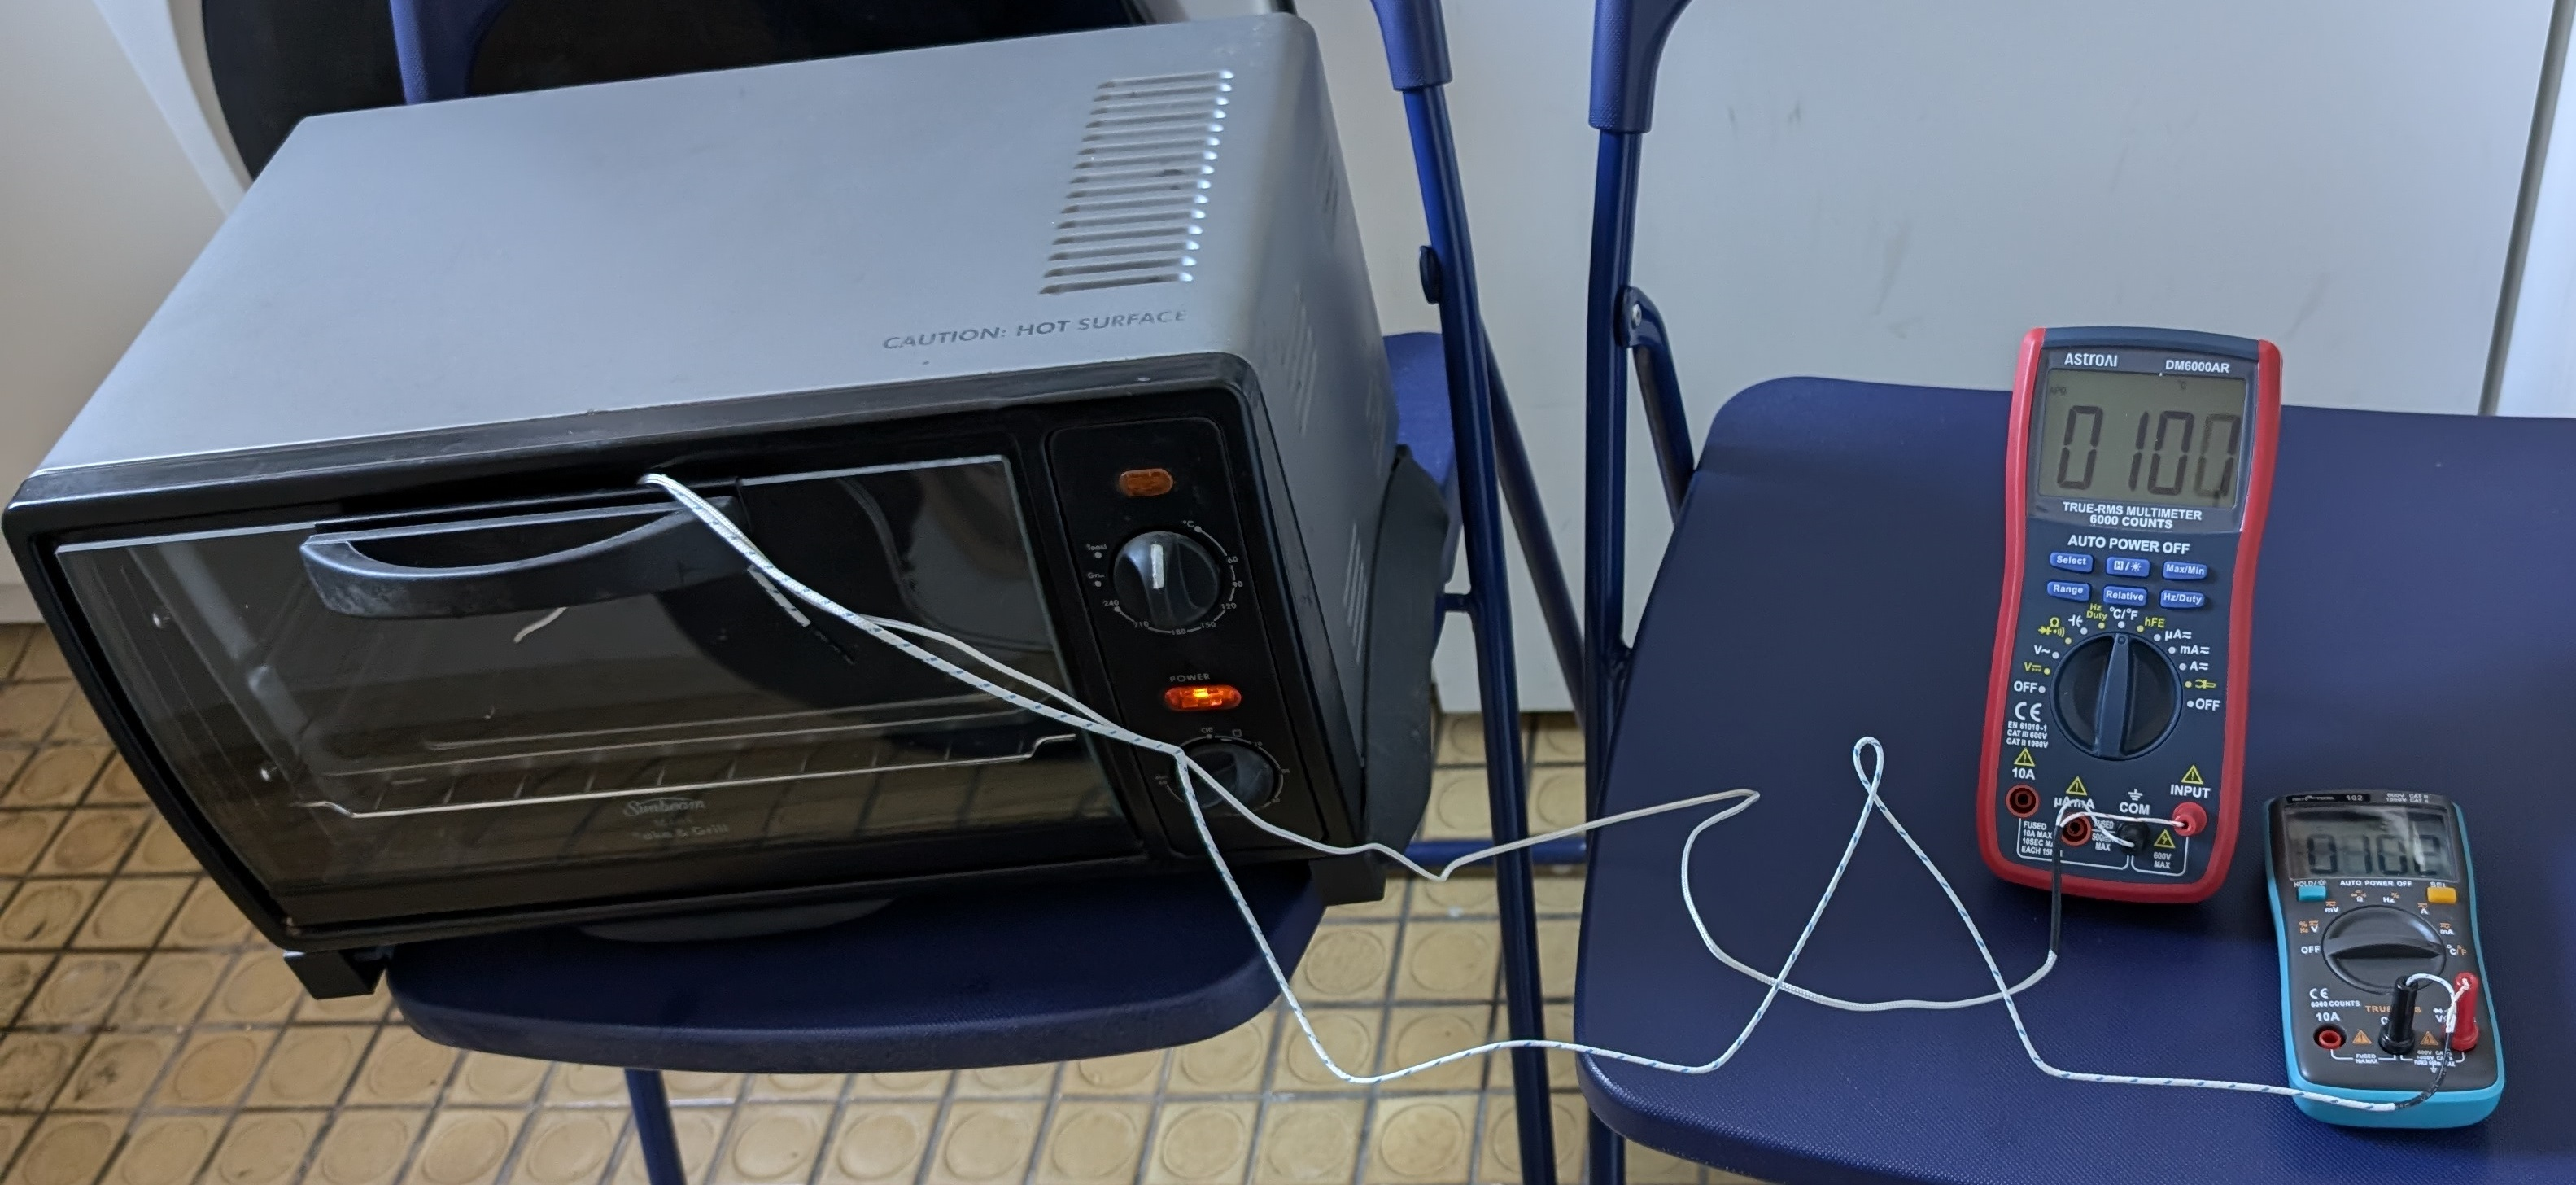
\includegraphics[width=0.75\textwidth]{images/oven_test.jpg}
  \caption{High-temperature testing setup}
  % \label{fig:temperature-testing-oven}
\end{figure}

A failure of this test occurs when the DAQ loses radio connection or transmits corrupted data for more than one minute, or if the system is not functional after the test.

\subsubsection{Low-Temperature Test}
\label{sec:ltemp-test-framework}
IIST recommended a qualification test where the CubeSat was placed into a thermal vacuum chamber for $\SI{2.5}{\hour}$ and was cooled to $\SI{-20}{\degreeCelsius}$. The CubeSat electronics were turned on and tested during the final $\SI{30}{\minute}$ of the test.

Due to time restrictions it was only possible to do a preliminary low-temperature test with a consumer freezer. To prevent condensation from developing on the electronics during the test, which would not occur in the thermal vacuum chamber, the electronics were placed in an airtight bag prior to the test and pressurised with pure nitrogen gas for $\SI{5}{\minute}$ to displace air containing moisture. Note that this would not replicate the thermal transfer conditions in a vacuum, but would at least qualify the temperature range of the components used.

\begin{figure}[H]
  \centering
  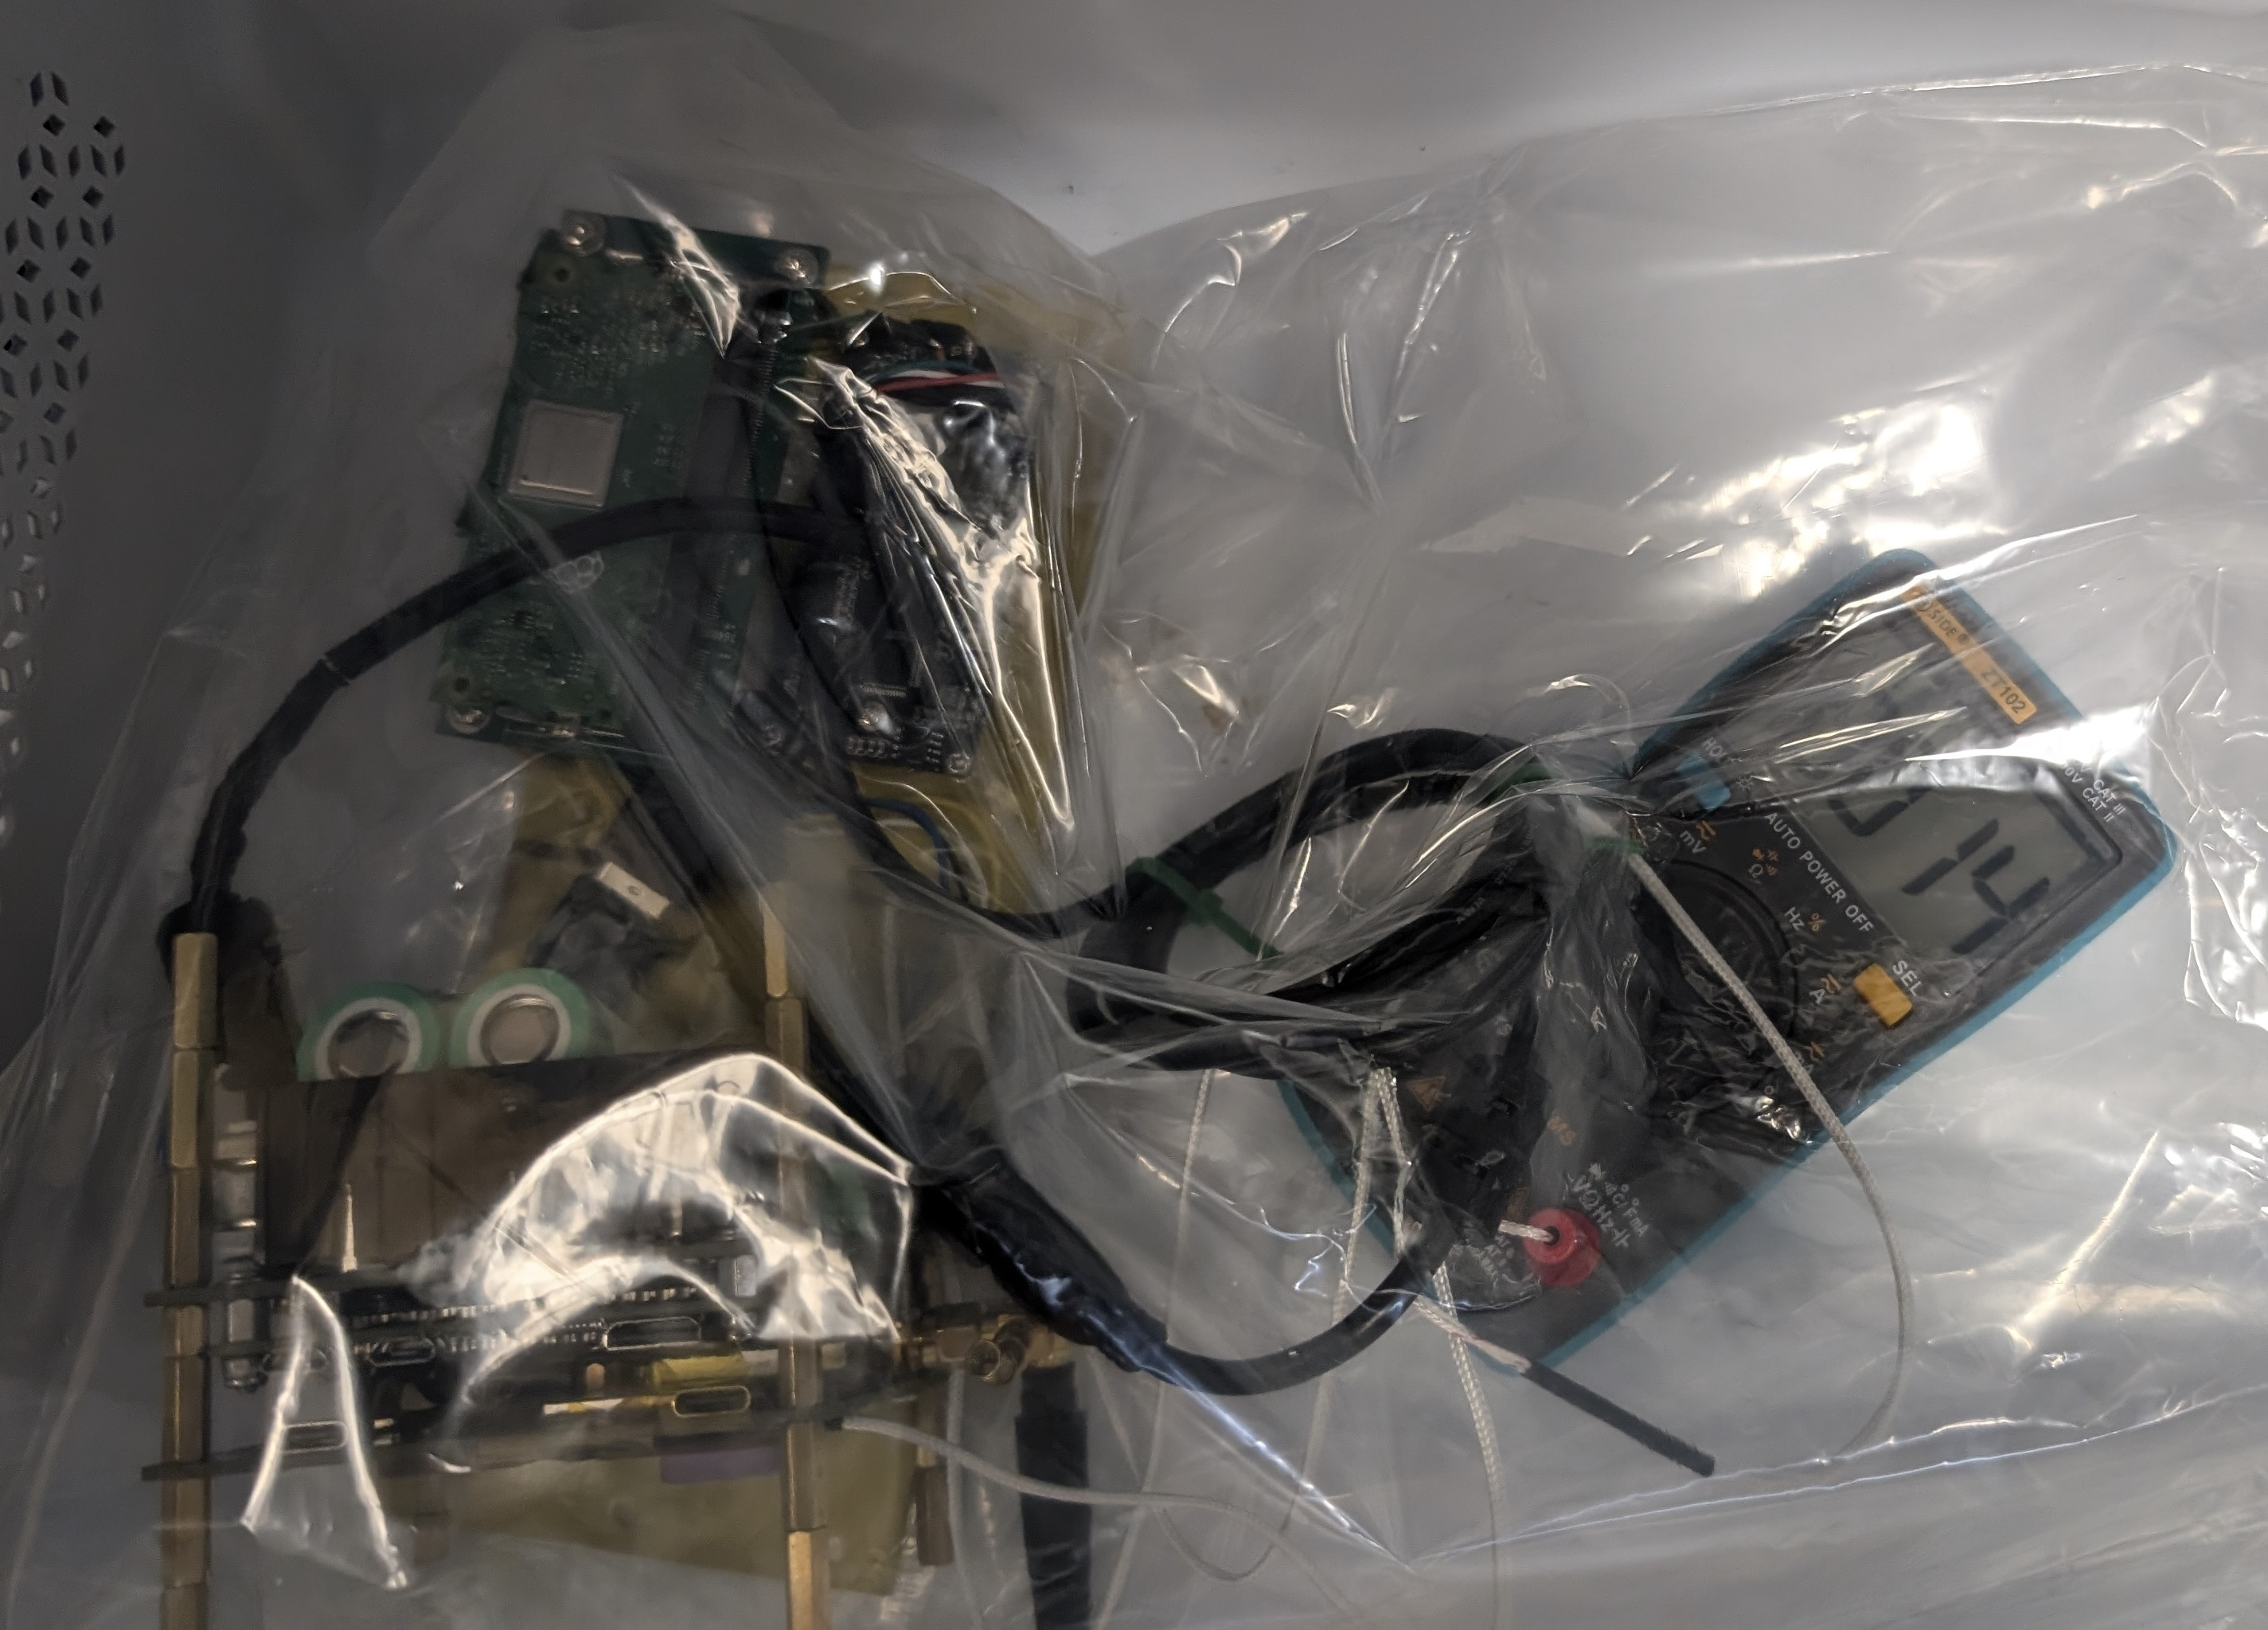
\includegraphics[width=0.75\textwidth]{images/fridge_test.jpg}
  \caption{Low-temperature testing setup}
  % \label{fig:temperature-testing-fridge}
\end{figure}

A failure of this test occurs when the DAQ loses radio connection or transmits corrupted data for more than one minute, or if the system is not functional after the test.

\subsection{Shaker Table Test}
\label{sec:shaker-table-test}

IIST recommended that the CubeSat be mechanically qualified using a single-axis electrodynamic shaker table using random vibration and half-sine shock tests.

\subsubsection{Random Vibration}

In the random vibration test, the CubeSat was fixed rigidly to an electrodynamic shaker table, then the table was programmed with the IIST recommended vibration profile specified in table \ref{tabl:random-vibration-profile-iist}. The vibration test occured for \SI{60}{\second} per axis and was repeated for all three axes.

\begin{table}[t]
  \centering
  \begin{tabular}{|c | c | c | c | c|}
    \hline
    \textbf{Frequency ($\si{\hertz}$)} & \textbf{PSD ($\si{\square\gacc\per\hertz}$)} & \textbf{$\si{\gacc}$ (RMS)} & \textbf{Duration ($\si{\second\per\siaxis}$)} & \textbf{Axis}               \\ \hline
    20                                 & 0.002                                        & \multirow{5}{*}{13.5}       & \multirow{5}{*}{60}                           & \multirow{5}{*}{Three axes} \\ \cline{1-2}
    60                                 & 0.002                                        &                             &                                               &                             \\ \cline{1-2}
    250                                & 0.138                                        &                             &                                               &                             \\ \cline{1-2}
    1000                               & 0.138                                        &                             &                                               &                             \\ \cline{1-2}
    2000                               & 0.034                                        &                             &                                               &                             \\ \hline
  \end{tabular}
  \caption{IIST recommended random vibration test profile for qualification of CubeSat for launch on POEM.}
  \label{tabl:random-vibration-profile-iist}
\end{table}


\begin{figure}[H]
  \centering
  \includesvg[width=0.8\linewidth]{images/random-qualification-level.svg}
  \caption{IIST recommended random vibration test profile for qualification of CubeSat for launch on POEM (profile defined in \ref{tabl:random-vibration-profile-iist}).}
  \label{fig:random-vibration-qualification-level}
\end{figure}

The IIST recommended random vibration test profile was used without modifications in the final shaker table testing.

A failure of this test occurs when the DAQ loses radio connection or transmits corrupted data for more than one minute, or if the system is not functional after the test.

% \subsubsection{Sine-Sweep}

% The CubeSat was fixed rigidly to an electrodynamic shaker table, then the table was programmed with the IIST recommended sine-sweep profile specified in table \ref{tabl:sine-sweep-profile-iist}. Frequencies between \SI{10}{\hertz} and \SI{100}{\hertz} were swept at a rate of \SI{4}{\octave\per\minute} and was repeated for all three axes.


% \begin{table}[H]
%   \centering
%   \begin{tabular}{|c|c|c|c|c|c|}
%     \hline
%     \multicolumn{2}{|c|}{\textbf{Longitudinal}} & \multicolumn{2}{c|}{\textbf{Lateral}} & \multirow{2}{*}{\textbf{Sweep Rate}} & \multirow{2}{*}{\textbf{Axis}}                                           \\ \cline{1-4}
%     \textbf{Frequency}                          & \textbf{Level}                        & \textbf{Frequency}                   & \textbf{Level}                 &                            &            \\ \hline
%     \SIrange{10}{16}{\hertz}                    & \SI{20}{\mmDA}                        & \SIrange{10}{16}{\hertz}             & \SI{12}{\mmDA}                 & \SI{4}{\octave\per\minute} & Three axes \\ \hline
%     \SIrange{16}{100}{\hertz}                   & \SI{10}{\gacc}                        & \SIrange{16}{100}{\hertz}            & \SI{6}{\gacc}                  & \SI{4}{\octave\per\minute} & Three axes \\ \hline
%   \end{tabular}
%   \caption{IIST recommended sine-sweep profile.}
%   \label{tabl:sine-sweep-profile-iist}
% \end{table}

% A failure of this test occurs when the DAQ loses radio connection or transmits corrupted data for more than one minute, or if the system is not functional after the test.

\subsubsection{Shock}

In the shock test, the CubeSat was fixed rigidly to an electrodynamic shaker table, then the table was programmed with the IIST recommended half-sine shock profile specified in table \ref{tabl:random-vibration-profile-iist}. The amplitude of the shocks had to be reduced in the test due to limitations of the shaker table.

The IIST recommended qualification level for the shock test is specified in table \ref{tabl:shock-test-iist}.

\begin{table}[H]
  \centering
  \begin{tabular}{|c|c|c|c|}
    \hline
    \textbf{Amplitude} & \textbf{Duration (ms)} & \textbf{Shock profile} & \textbf{Axis}                          \\ \hline
    \SI{50}{\gacc}     & 10                     & Half sine              & Single-axis shocks, for all three axes \\ \hline
  \end{tabular}
  \caption{IIST recommended shock test profile for qualification of CubeSat for launch on POEM.}
  \label{tabl:shock-test-iist}
\end{table}

A failure of this test occurs when the DAQ loses radio connection or transmits corrupted data for more than one minute, or if the system is not functional after the test.

\subsection{Vehicle Tests}

\subsubsection{Drone Test Flights}

Drone tests were used as a qualification platform for the HPR launch since drone tests:

\begin{enumerate}
  \item Use the expertise of the UWA Aviation Laboratory, which is participating in the project.
  \item Are repeatable, whereas the rocket test can only feasibly be done once per launch season.
  \item Have greater control over the position compared to the suborbital rocket launch and will better qualify the machine vision processes on the camera payload.
\end{enumerate}

The drone test evaluated the communications between the camera payload and the communications downlink stability in real time. A successful test involved receiving at least one frame from the camera payload at a reasonable quality.

\subsubsection{High-Power Rocket Test Flight}

The high-power rocket (HPR) test flight was used as an experimental qualification method for the CubeSat. This DAQ is used to evaluate the effectiveness of the HPR flight by using accelerometers, but the HPR flight also serves as a milestone for evaluating the effectiveness of this DAQ for this type of application.

\subsection{Experiment Evaluation}

The first condition for the experiment to be successful was if a conclusion could be reached on if HPR is a viable alternative qualification method using only the response of the HPR and shaker table tests.

Since this design used lower cost MEMS accelerometer as the vibration measurement device, this had to be validated. It will be assumed that the accelerometers on the shaker table have been calibrated adequately. By comparing the response observed by the shaker table vibration sensors to the response observed by the MEMS accelerometer, it will be possible to evaluate the effectiveness over the spectrum of vibrations the DAQ encounters during flight.

\section{Version One of DAQ}

The design process allows for multiple versions of the DAQ to be designed, subject to time and budget constraints.

\subsection{Overview of First Design}

The first design had three boards: EPS, radio and OBDH.

The OBDH was based on a STM32L476 microcontroller and the \SI{8}{\giga\bit} THGBMJG6C1LBAIL embedded multimedia card (eMMC). All connections out of the microcontroller going to other boards were using the RS-485 physical layer. This design also was intended to be used in a dual redundant pair. A ZED-F9P differential GNSS receiver was used in this design. Other elements of the design were not changed between the first and second revision.

The microcontroller was programmed in C using the STM32 hardware abstraction library (HAL) and using FreeRTOS as a realtime operating system to manage scheduling.

\subsection{Evaluation of First Design}

\begin{itemize}
  \item The STM32L476 did not have enough resources to move data from the sensors and camera payload to the payload at an adequate speed. A benchmark using CrystalDiskMark, in table \ref{tabl:daq-v1-diskmark} shows that the maximum throughput is $\SI{0.84}{\mega\byte\per\second}$, and while only 60\% of the throughput is being used as shown in table \ref{tabl:daq-v1-sensor-datarate}, between reading from the data sources and writing to the storage there is not enough resources in practice to do this at an adequate speed, resulting in the maximum sampling rate of the sensors to be limited.
  \item There were issues using the 4-bit mode on the eMMC, which limited write and read speeds.
  \item Due to space limitations on the rocket, it was not possible to have two redundant systems. The next revision would use only one DAQ.
  \item By the end of this section, it was understood that centimetre level positioning was not required to obtain good results from the camera system.
  \item A preliminary test with the camera payload showed that the RS-485 transceiver was able to successfully receive image data from the camera payload, but it was not able to write the data to the eMMC or the radio at an adequate rate.
  \item The preliminary test also showed that the EPS was adequate for delivering power to the camera payload.
  \item Good GNSS data was received from the GNSS board.
  \item The RFD900x performed well when tested alone without writing to the eMMC.
  \item At the end of this revision it was concluded that the STM32 platform was not flexible enough to complete the research objectives in time.
\end{itemize}

\begin{table}[H]
  \centering
  \begin{tabular}{|c|c|L{0.6\linewidth}|}
    \hline
    \textbf{Data source} & \textbf{Data rate}                  & \textbf{Notes}                                                                                                   \\\hline
    LSM6\-DSOX           & $\SI{0.41}{\mega\byte\per\second}$  & $16$ byte structs are generated at $\SI{6664}{\hertz}$ for both acceleration and gyroscope data for two sensors. \\\hline
    ADXL\-375            & $\SI{0.038}{\mega\byte\per\second}$ & $20$ byte structs generated at $\SI{1}{\kilo\hertz}$ for two sensors.                                            \\\hline
    Camera payload       & $\SI{0.054}{\mega\byte\per\second}$ & $\SI{460800}{\baud}$                                                                                             \\\hline
    \textbf{TOTAL}       & $\SI{0.502}{\mega\byte\per\second}$ & $60\%$ of maximum sequential write bandwidth.                                                                    \\\hline
  \end{tabular}
  \caption{Data sources and their data rates.}
  \label{tabl:daq-v1-sensor-datarate}
\end{table}

\begin{table}[H]
  \centering
  \begin{tabular}{|c|c|c|}
    \hline
    \textbf{Test}                 & \textbf{Read [MB/s]} & \textbf{Write [MB/s]} \\\hline
    SEQ1M Q1T1 (1 task, 1 thread) & 0.84                 & 0.84                  \\\hline
    % RND4K Q32T1 (32 tasks, 1 thread)  & 0.81  & 0.70\\\hline
    RND4K Q1T1 (1 task, 1 thread) & 0.75                 & 0.66                  \\\hline
  \end{tabular}
  \caption{CrystalDiskMark benchmark of DAQ v1.}
  \label{tabl:daq-v1-diskmark}
\end{table}

\subsection{First Revision Implications}

The EPS, GNSS receiver and radio designs were left unchanged since they performed well during preliminary testing.

However, the OBDH was completely changed to use a Raspberry Pi Zero W in the second revision. This was because a microcontroller was hard to debug due to a limited number of breakpoints and a lack of isolation between tasks in FreeRTOS which resulted in difficult to debug issues. A Raspberry Pi has a Linux-based operating system, which is easier to develop for since tools such as GDB can be used for debugging, and processes isolate errors from affecting other processes. The Raspberry Pi also has more resources and should not result in the poor write speeds observed on the first OBDH.

Some systems were simplified, such as the differential GNSS not being used on the final DAQ. RS-485 was also removed for board to board communication, except between the camera payload and the DAQ, since it was unnecessary given the short distance between DAQ boards.

\chapter{Final Design of DAQ}

The final DAQ design is implemented using the design process described in \secref{sec:design-process}.

\section{Overview of PCBs}

Three PCB projects are created for the three boards in the final design:
\begin{itemize}
  \item Power and OBDH (referred to as DAQ)
  \item GNSS receiver
  \item Accelerometers
\end{itemize}

As stated, PCB rules were set according to the JLCPCB capabilities page.

\subsection{PCB Sizes}
A PCB size of \SI{80 x 80}{\milli\metre} was used for the  boards since this was the maximum size available for the PCB inside the CubeSat. The DAQ board uses this size since the batteries are mounted on the reverse side of the board, and require a lot of board area to mount. The GNSS receiver board uses this size since larger PCB areas result in higher gain for the patch antennas used for receiving GNSS signals. For the MEMS accelerometers, a PCB of \SI{22 x 22}{\milli\metre} was chosen as it was the minimum size possible to fit both accelerometers and mounting holes, and minimising the PCB area maximises the resonant frequency of the accelerometers.

\subsection{PCB Stackups}
Four layer stackups are used for the DAQ and GNSS boards since these were cheap to manufacture at JLCPCB for boards under \SI{100x100}{\milli\meter}, and they were simpler to route due to more layers. The DAQ used a standard signal-ground-power-signal stackup. This was chosen since the DAQ board contains many parts and having a dedicated power and ground plane made routing simpler and improved the EMI performance of the PCB. The GNSS board contained few components and used a stackup of four ground layers which covered the full PCB to maximise the gain of the patch antennas. The accelerometer board used a two-layer signal-signal stackup since there were few components to route and to save cost.

All boards used a 7628 substrate since this was the lowest cost substrate and acceptable since the highest frequencies routed on the PCBs were the L1 signal for GNSS, which is a relatively low \SI{1575.42}{\mega\hertz}. As shown in figure \ref{fig:7628-fr4-loss}, the loss for a microstrip is under \SI{1}{\decibel} at \SI{2}{\giga\hertz} \cite{hamilton2007humidity}, which is acceptable.

\begin{figure}[H]
  \centering
  \includesvg[width=\linewidth]{images/fr4_attenuation.svg}
  \caption{S21 attenuation parameters of several dielectrics for a \SI{50}{\ohm} microstrip. Compared to the high-performance Rogers 4350 dielectric, there is negligible difference in attenuation at low frequencies. Adapted from \cite{hamilton2007humidity}}
  \label{fig:7628-fr4-loss}
\end{figure}

All boards used hot air solder levelling (HASL) lead-tin coating due to its low cost, and since this PCB did not require flat surface finishes since relatively large components were being soldered on to the PCB, and since these boards were not commercial boards that were subject to environmental requirements.

\section{Electrical Power System (EPS)}

\subsection{Power Budget}

The power budget of the DAQ and the required power supply for the payload was created for the final design, as shown in table \ref{tabl:eps-power-budget-final}.

\begin{table}[H]
  \centering
  \begin{tabular}{|c|c|L{0.2\linewidth}|c|L{0.2\linewidth}|}
    \hline
    \textbf{Item}                    & \textbf{Voltage (\si{\volt})} & \textbf{Max unit current (\si{\milli\ampere})} & \textbf{Quantity} & \textbf{Max current (\si{\milli\ampere})} \\
    \hline
    Payload-under-test               & 5                             & 3000                                           & 1                 & 3000                                      \\
    Pi Zero                          & 5                             & 1300 \cite{raspberry-pi-hardware-doc}          & 1                 & 1200                                      \\
    RFD900x                          & 5                             & 1000 \cite{rfdesign2020rfd900x}                & 1                 & 1000                                      \\
    NEO-M9N                          & 3.3                           & 100 + 50 \cite{ublox2023neo_m9n_datasheet}     & 1                 & 150                                       \\
    % ZED-F9P                          & 3.3                           &                                                   & 1                 &                                       \\
    LSM6\-DSOX                       & 3.3                           & 0.55 \cite{lsm6dso-datasheet}                  & 2                 & 1.1                                       \\
    ADXL\-375                        & 3.3                           & 0.145 \cite{analog2014adxl375}                 & 2                 & 2.9                                       \\
    % E32-900M30S                      & 3.3                           & 650                                               & 1                 & 650                                          \\
    SP3485EN                         & 3.3                           & 2 \cite{maxlinear2021sp3485}                   & 1                 & 2                                         \\
    XR20M1172                        & 3.3                           & 0.5 \cite{maxlinear2022xr20m1172}              & 2                 & 1                                         \\
    \hline
    \textbf{Total (\SI{3.3}{\volt})} & -                             & -                                              & -                 & 157                                       \\
    \textbf{Total (\SI{5}{\volt})}   & -                             & -                                              & -                 & 5200                                      \\
    \hline
  \end{tabular}
  \caption{Operating voltage and current consumption of devices connected to EPS.}
  \label{tabl:eps-power-budget-final}
\end{table}

\subsection{Battery Selection}

COTS 18650 lithium-ion batteries were chosen as the energy source for the DAQ. The advantages of this battery satisfy the criteria in \secref{sec:battery-selection} and include:

\begin{itemize}
  \item The 18650 format encases the battery in a rigid metal cylinder which is well-suited for the space environment \cite{knap2020review}. Battery formats which use a flexible pouch, like most lithium-polymer cells, are more prone to outgassing in the vacuum of space \cite{knap2020review}.
  \item Compared to other rechargeable battery solutions such as \ce{Ni}-\ce{Cd} and \ce{Ni}-\ce{H2}, \ce{Li}-ion batteries have improved temperature range, energy density and specific energy and cycle life \cite{pathak2023review}.
  \item COTS \liion batteries are a mature battery format due to widespread use in consumer products \cite{pathak2023review}.
  \item Extensive flight heritage as they have been proven in other CubeSat missions \cite{knap2020review}, and are being used on flagship NASA missions, such as Europa Clipper \cite{krause2021performance}.
  \item COTS batteries are produced at scale for commercial markets and are lower cost compared to specialised aerospace batteries.
\end{itemize}

Manufacturers produce a variety of types of \liion batteries with different chemistries, which affect parameters including internal resistance, discharge and charging temperature range and capacity.

The Samsung INR18650-25R \liion battery was chosen for the DAQ platform due to
\begin{itemize}
  \item Previous flight heritage on CubeSats \cite{marcelino2021orbit}.
  \item Operation over a large temperature range of \SIrange{-20}{75}{\degreeCelsius} and has been proven to be stable at \SI{130}{\degreeCelsius} \cite{samsung2014}.
  \item Good capacity of \SI{2500}{\milli\ampere\hour} and high maximum discharge rate of \SI{20}{\ampere} \cite{samsung2014}.
  \item Low cost.
\end{itemize}

\subsection{Battery Pack}
As stated in the high-level design (\Secref{sec:hl-power-electronics}), a 1S lithium-ion battery pack was selected. In the final design, three batteries were placed in parallel to form a 1S3P battery pack. Three 18650 cells were selected since this is the maximum number of cells which can fit on a \SI{80 x 80}{\milli\metre} PCB using a 3 cell 18650 battery holder. This connector holds batteries using a leaf spring.

The 1S3P battery pack was mounted on the reverse side of the PCB due to the amount of space it consumes, as shown in figure \ref{fig:batteries-pcb}.

\begin{figure}[H]
  \centering
  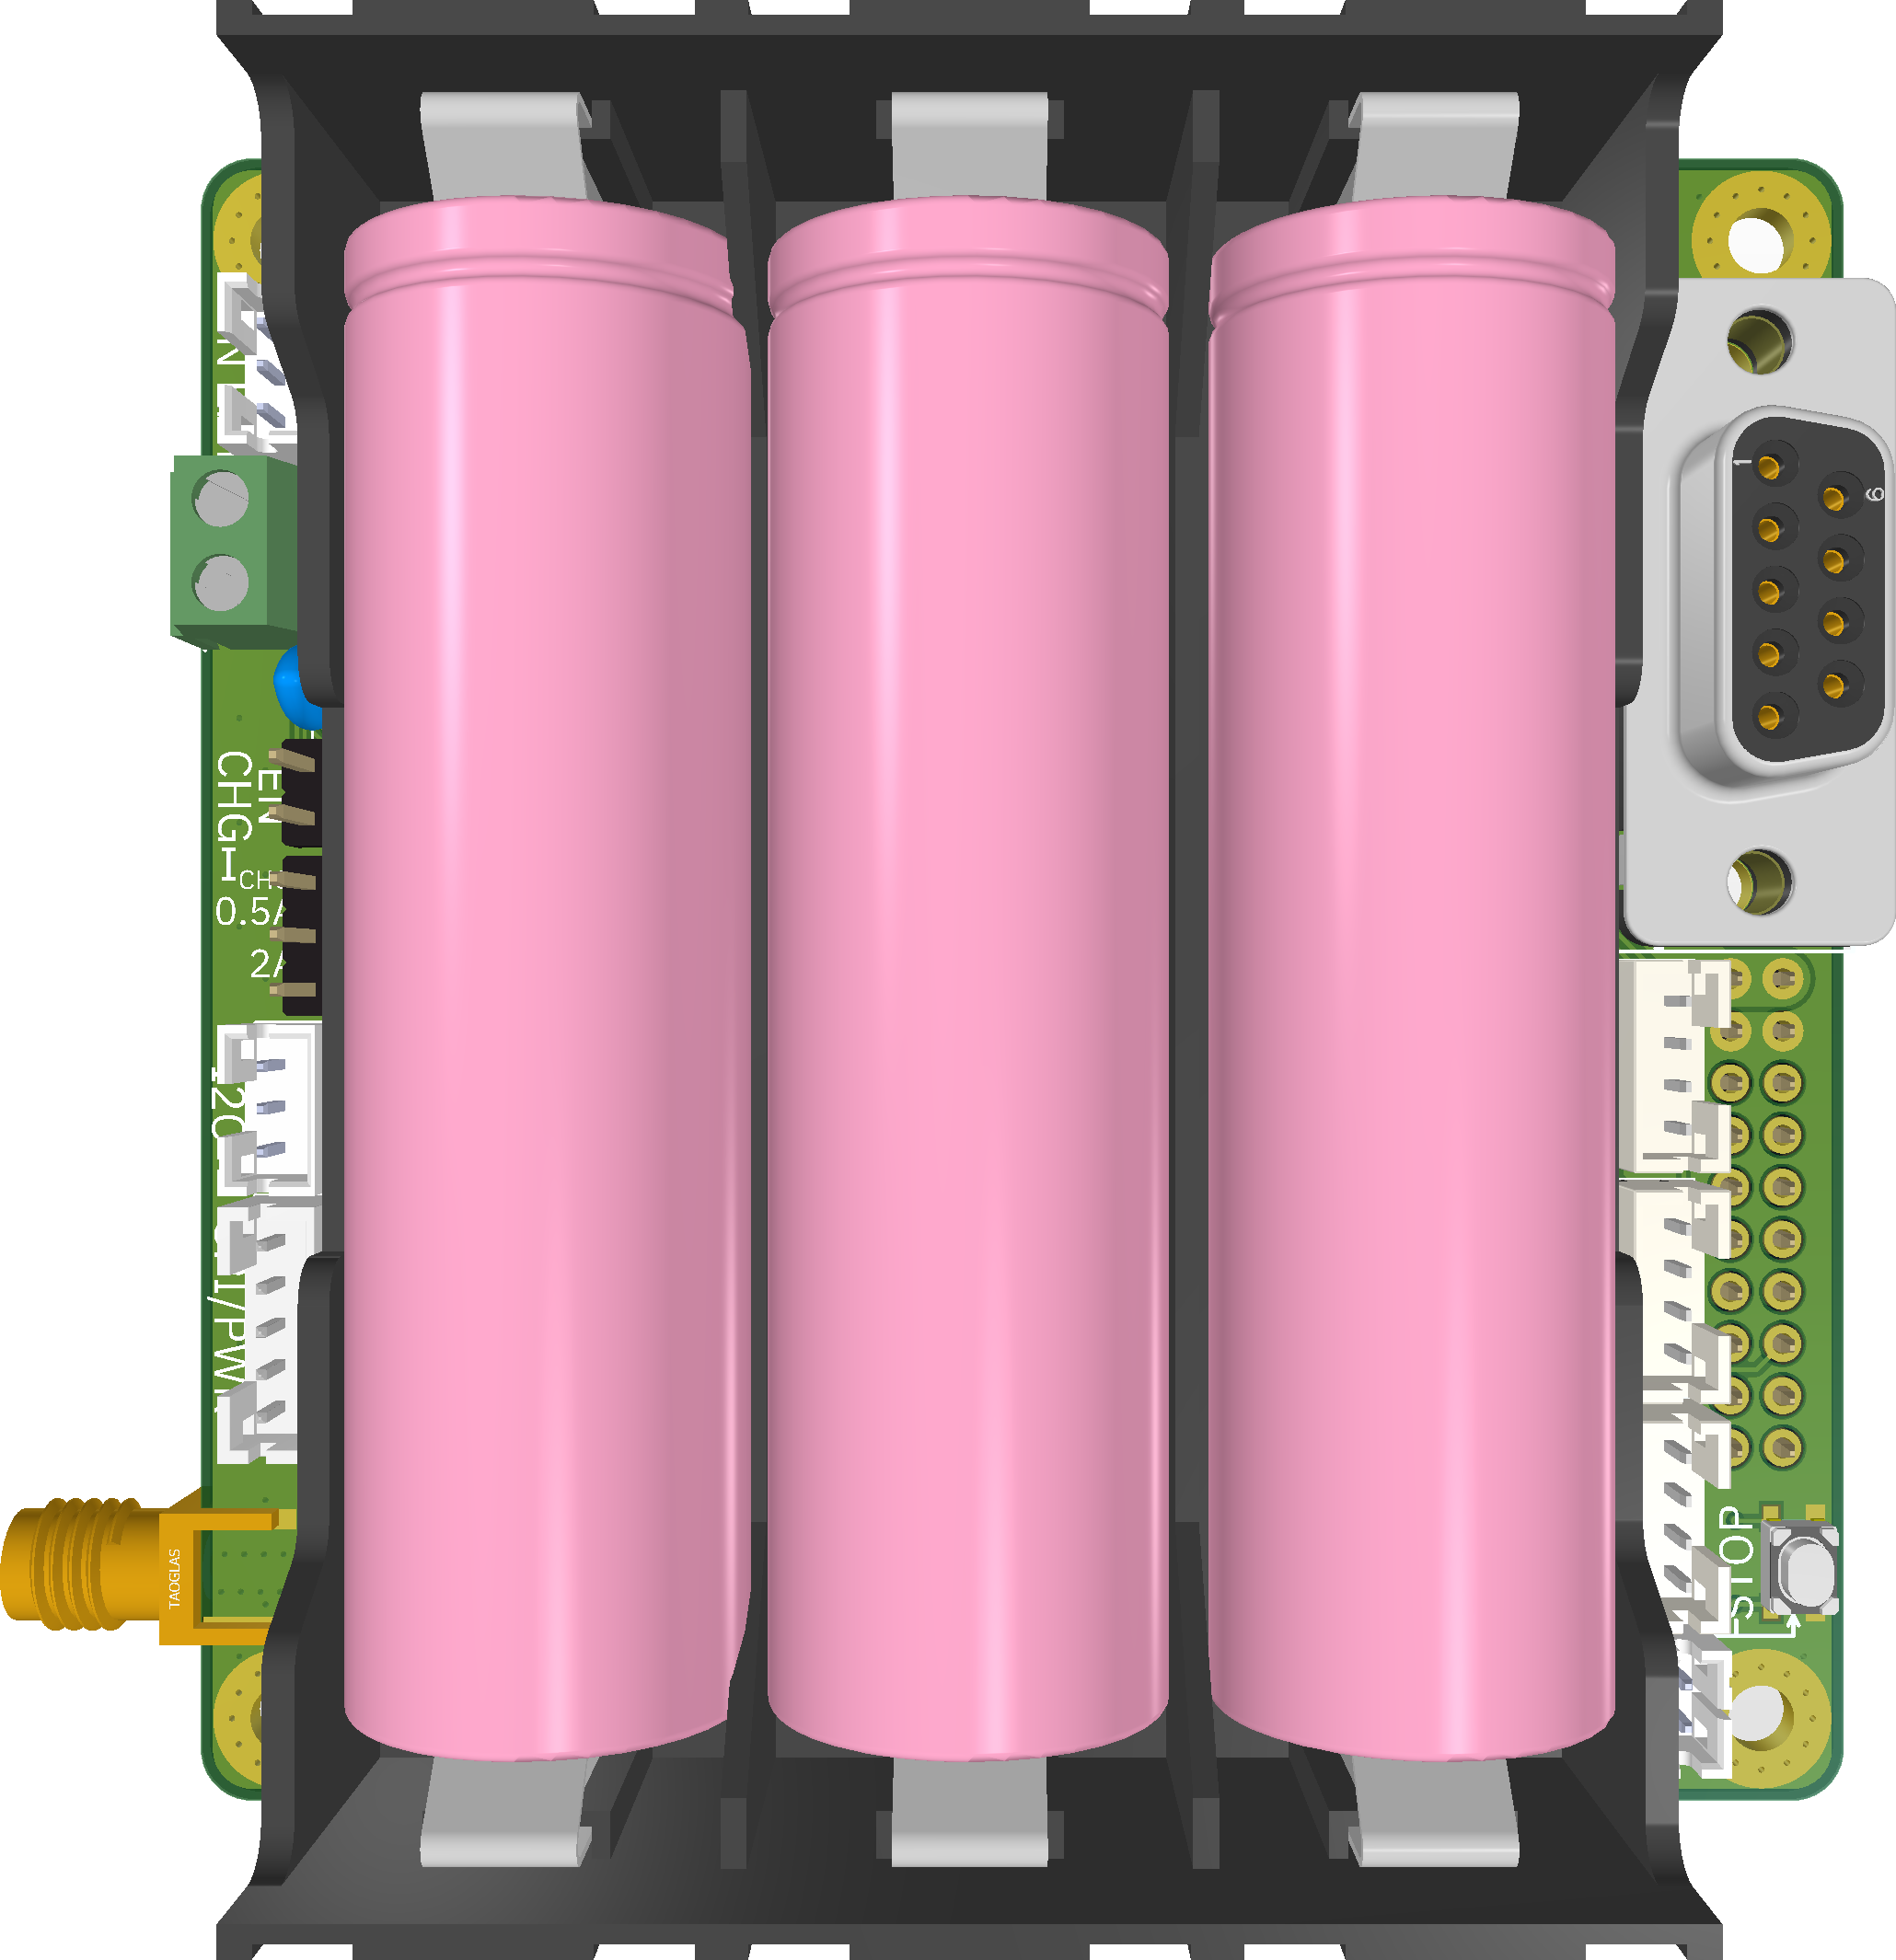
\includegraphics[width=0.8\linewidth]{images/batteries_PCB.png}
  \caption{Battery mounting on reverse side of DAQ PCB.}
  \label{fig:batteries-pcb}
\end{figure}

The battery pack can be charged by connecting \SI{5}{\volt} power to a charging terminal block. Two \SI{1}{\ampere} TP4056 linear \liion battery chargers were connected in parallel to the battery pack to allow a maximum charging current of \SI{2}{\ampere}.

\subsection{\SI{5}{\volt} Power Conditioning Design and Simulation}

The Texas Instruments TPS61022 boost converter was selected for this 1S system. It had a working voltage range of \SIrange{1.8}{5.5}{\volt} which was suitable for a 1S3P \liion battery pack with a working voltage range of \SIrange{2.5}{4.2}{\volt}, a maximum output current of over \SI{3}{\ampere} and can be configured to have an output voltage of \SI{5}{\volt} which was ideal for the DAQ and the camera payload \cite{ti2021tps61022}. A DC-DC switching converter was selected since it has high efficiency above 90\% throughout the input voltage of a standard 1S battery pack \cite{ti2021tps61022}. The TPS61022 had an operating temperature range of \SIrange{-40}{150}{\degreeCelsius} which was adequate for thermal qualification \cite{ti2021tps61022}. This satisfies the requirements described in \secref{sec:hl-power-electronics}.

The inductor selected for the converter subsystem is the ASPI-0630HI-1R0M-T15, which was a \SI{1}{\micro\henry} coil with a low DC resistance of \SI{10}{\milli\ohm}. The coil had a saturation current of \SI{20.5}{\ampere} which was above the \SI{8}{\ampere} maximum switching current. To make manufacturing simpler, the voltage divider was changed from $R_1=\SI{732}{\kilo\ohm}$ and $R_2=\SI{100}{\kilo\ohm}$ to use $R_1=\SI{750}{\kilo\ohm}$ and $R_2=\SI{100}{\kilo\ohm}+\SI{2}{\kilo\ohm}$ since these resistor values are available on JLCPCB. A \SI{1}{\pico\farad} compensation capacitor was also added. To evaluate the effects of these choices, the converter was simulated in LTspice with a single fully charged lithium-ion battery as the input.

\begin{figure}[H]
  \centering
  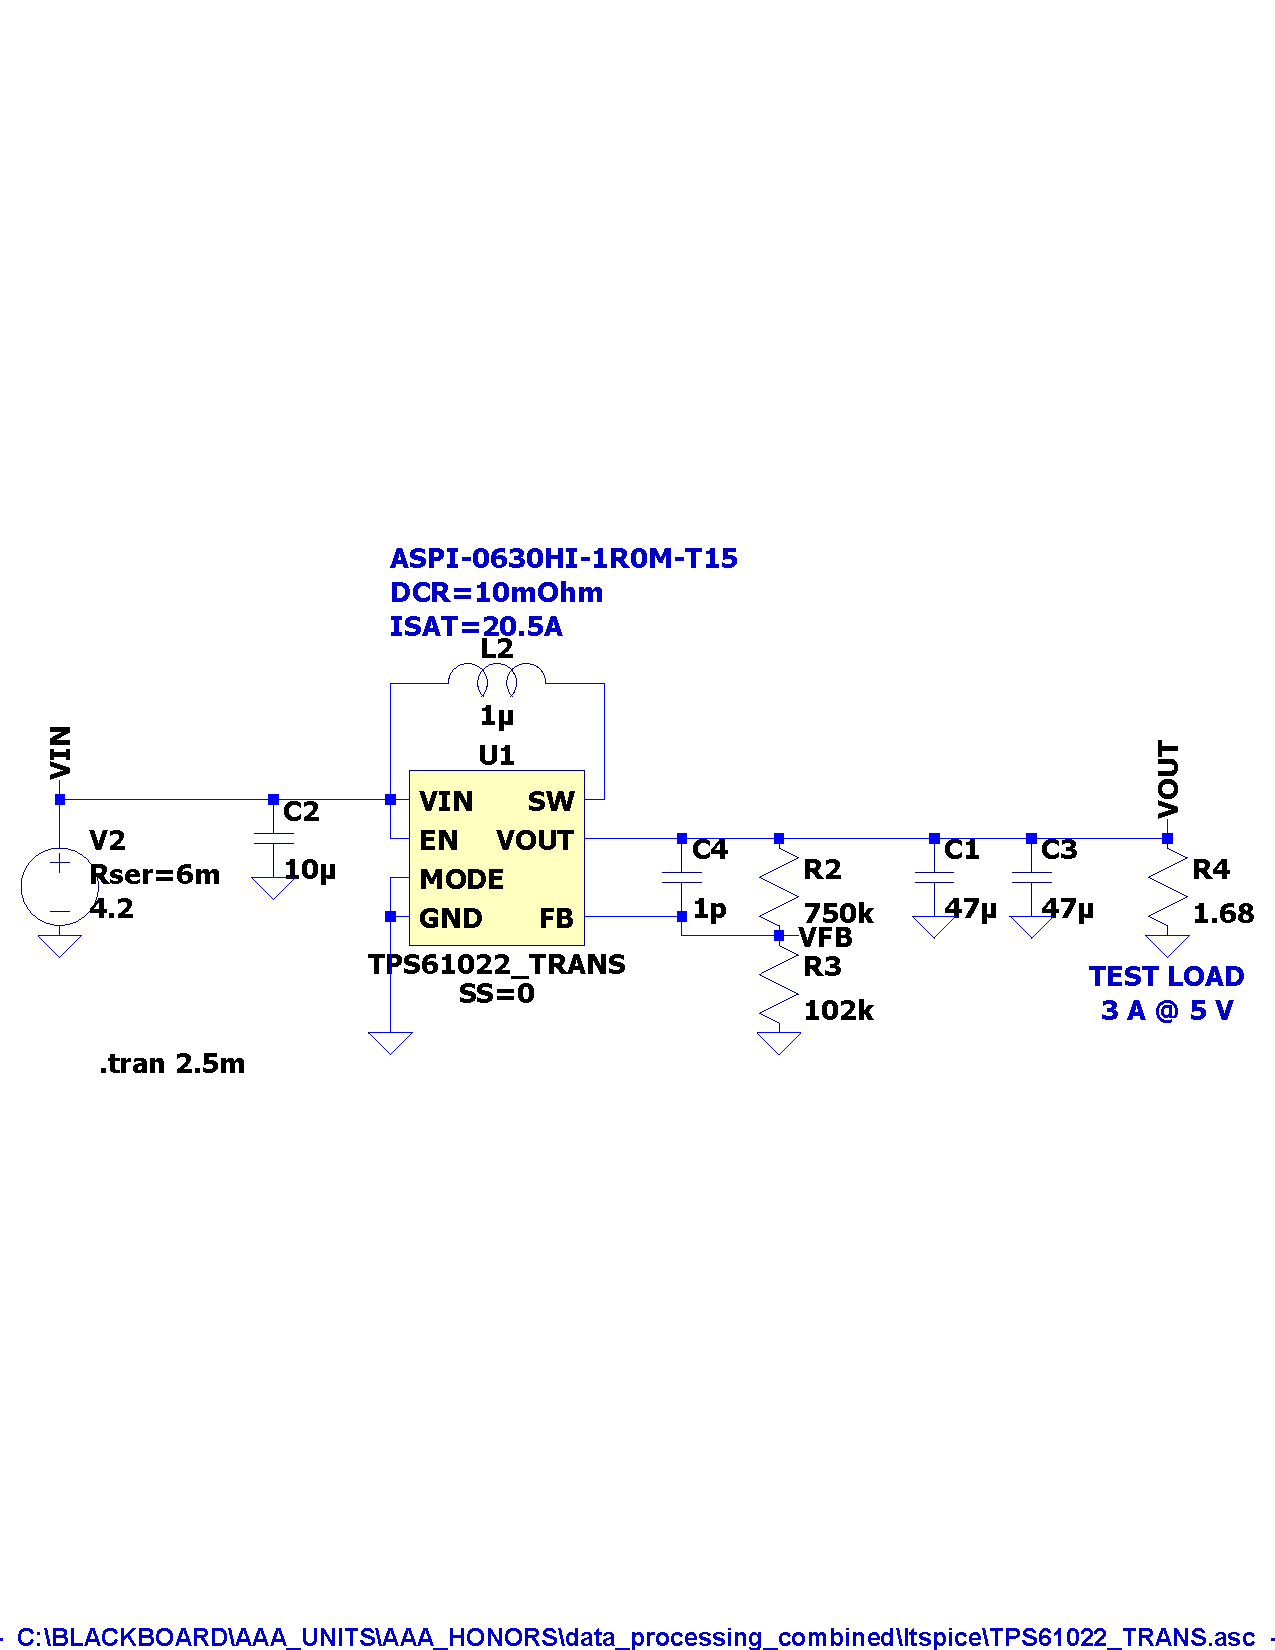
\includegraphics[trim=0 8.5cm 0 8cm, clip, width=\linewidth]{images/TPS61022-simulation.pdf}
  \caption{LTspice schematic representation of TPS61022.}
  \label{fig:TPS61022-schematic-ltspice}
\end{figure}

\begin{figure}[H]
  \begin{subfigure}{0.495\textwidth}
    \centering
    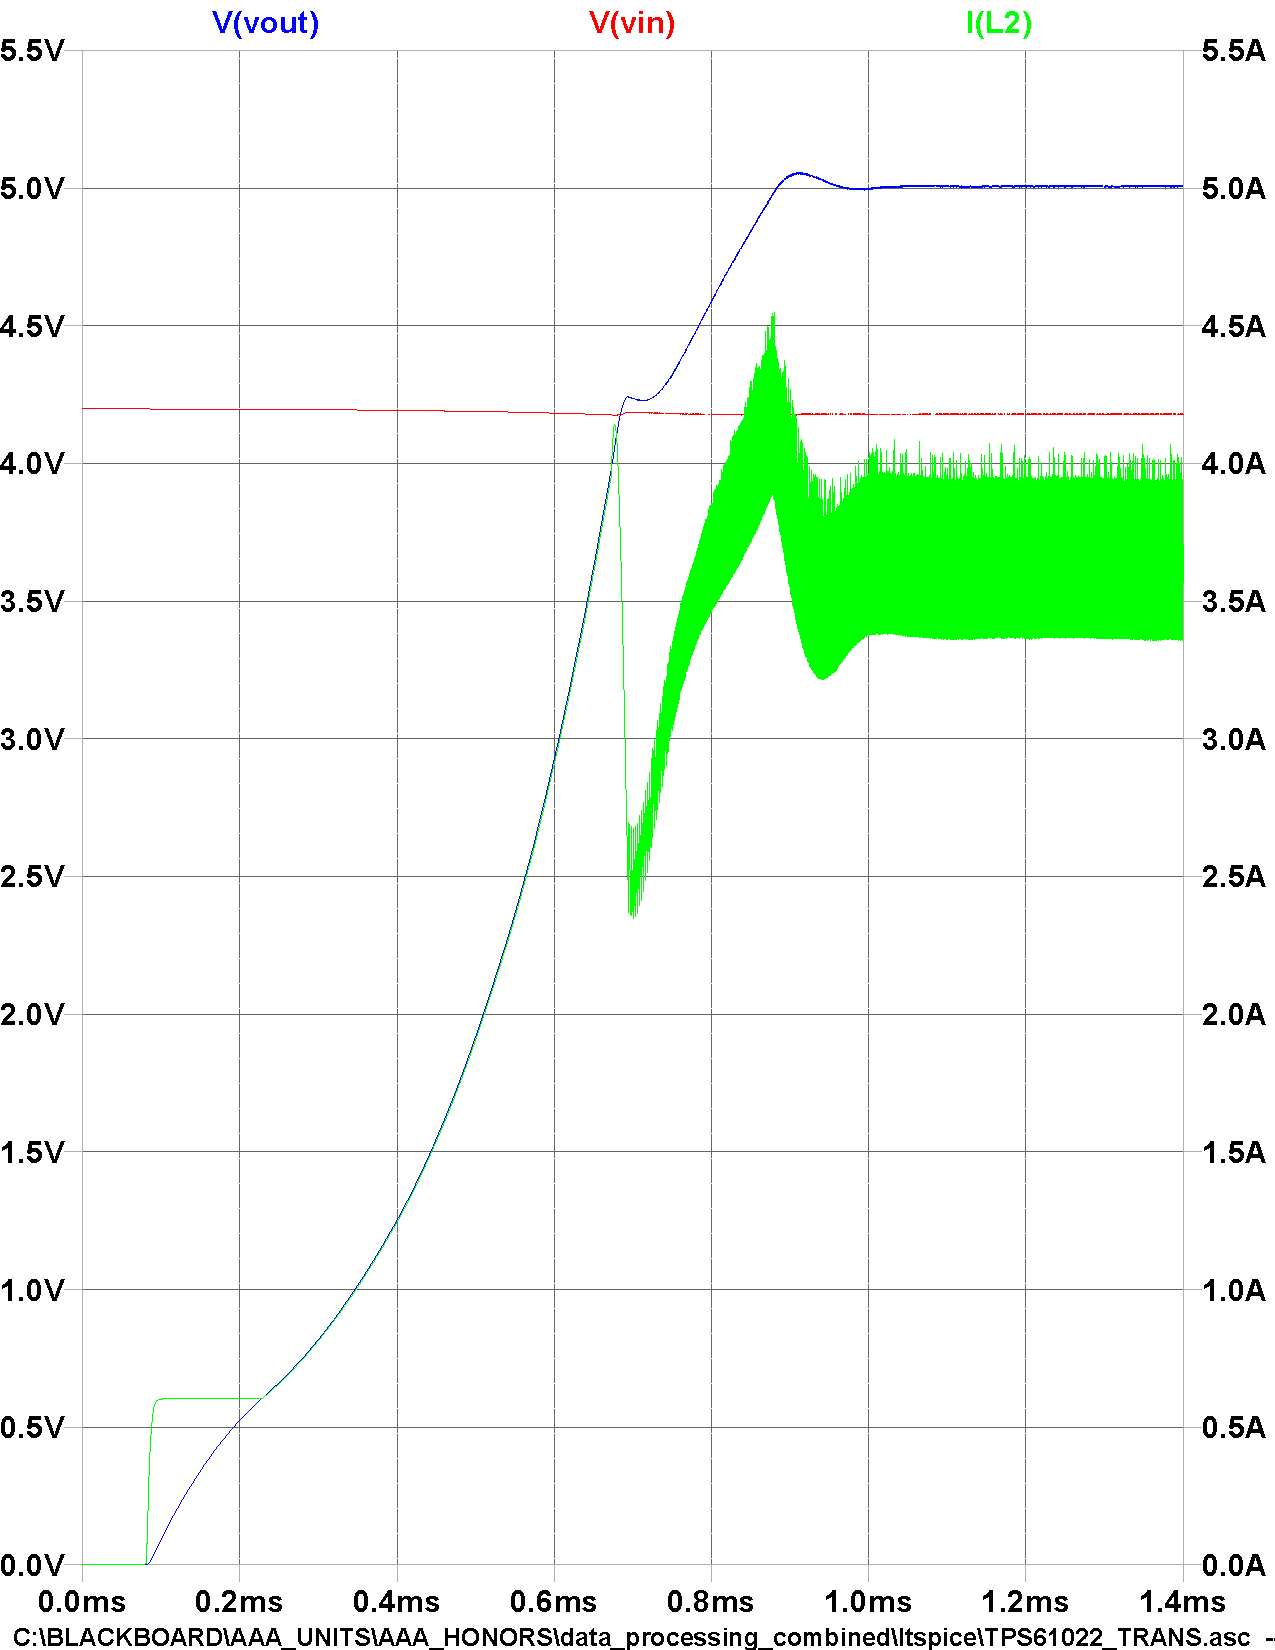
\includegraphics[width=\linewidth]{images/TPS61022-simulation-plot.pdf}
    \caption{Startup and steady-state behaviour.}
  \end{subfigure}
  \begin{subfigure}{0.495\textwidth}
    \centering
    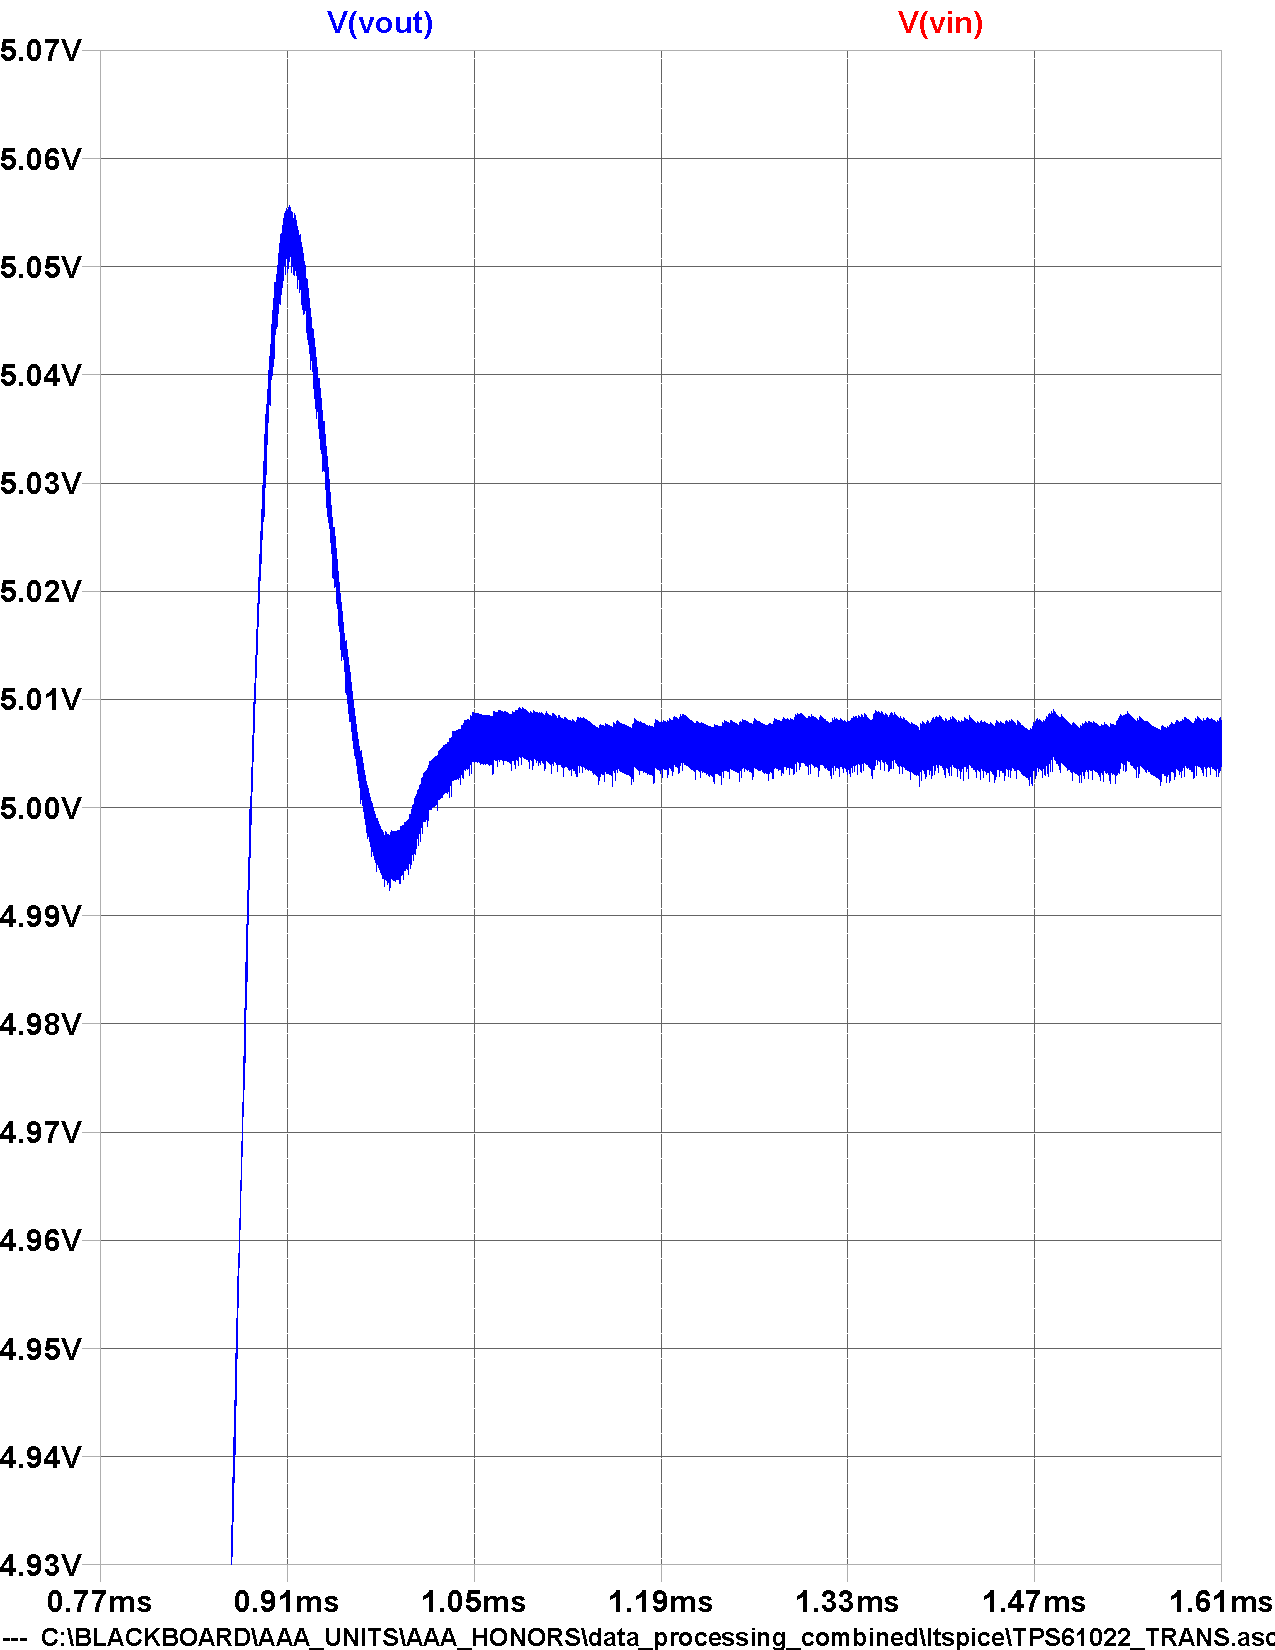
\includegraphics[width=\linewidth]{images/TPS61022-simulation-plot-overshoot.pdf}
    \caption{Close-up of startup transient and steady-state behaviour.}
  \end{subfigure}
  \caption{Simulation of the TPS61022 in LTspice using component values close to the datasheet as shown in figure \ref{fig:TPS61022-schematic-ltspice}.}
  \label{fig:TPS61022-simulation-ltspice}
\end{figure}

As shown in figure \ref{fig:TPS61022-simulation-ltspice}, during startup there was a small voltage overshoot of \SI{0.06}{\volt}, but this was negligible and well within the tolerance of the components. The steady-state output voltage has a mean of \SI{5.006}{\volt} and a peak to peak ripple voltage of \SI{7}{\milli\volt}, or a ripple of 0.15\%, which was more than adequate for this application since it was mainly digital logic.

The simulation also showed that the power system would work up to \SI{3}{\ampere}, which was the output current required to emulate the power capabilities of POEM. Two TPS61022 boost converters were used in the final design: one was  dedicated for the payload-under-test, and the other was for the DAQ. This allowed the payload to be able to receive the maximum current able to be provided by POEM, and also isolated failures in either system from affecting the other.

\subsection{Internal \SI{3.3}{\volt} Power Conditioning}

The DAQ internally used \SI{3.3}{\volt} for some components, however this system only uses a maximum of \SI{157}{\milli\ampere} therefore efficiency is a lower factor and a linear regulator was chosen. This solution resulted in a power loss of \SI{270}{\milli\watt}, which was considered insignificant compared to the maximum power output of the \SI{5}{\volt} system (\SI{26}{\watt}). %TODO:

An Advanced Monolithic Systems AMS1117-3.3 linear regulator was chosen due to its cheap pricing on JLCPCB of only \aud 0.20 and since it has been used in past designs with success. It has a high dropout voltage of \SI{1.1}{\volt}, which was acceptable for the \SI{5}{\volt} input \cite{ams2007ams1117}. The AMS1117 had an operating temperature range of \SIrange{-40}{125}{\degreeCelsius} which was adequate for thermal qualification \cite{ams2007ams1117}.

This regulator had been validated in previous boards, therefore implementing this subsystem only required cloning the schematic and layout to the design.

\subsection{EPS Subsystem Design}

Each of the subsystems were arranged as shown in figure \ref{fig:power-conditioning}. The payload and DAQ were powered off separate boost converters, since the payload can potentially use the full \SI{3}{\ampere} capacity of a single boost converter. The output of the two converters are not combined to ensure a failure on one power rail would not affect the other. Regulation of the \SI{3.3}{\volt} supply occurs after boosting to \SI{5}{\volt} since the high dropout voltage of the regulator prevents it operating directly from the battery.

\begin{figure}[H]
  \centering
  \includesvg[width=\linewidth]{images/power conditioning.svg}
  \caption{Electrical power system (EPS) and output voltages}
  \label{fig:power-conditioning}
\end{figure}

\subsection{Integration into DAQ}

A single schematic was created for the TPS61022 based off the successful LTspice simulation and instantiated twice in the root schematic. A PCB layout based on Figure 10-1 from the datasheet was used and is shown in figure \ref{fig:TPS61022-layout} \cite{ti2021tps61022}.

\begin{figure}[H]
  \begin{subfigure}{0.495\textwidth}
    \centering
    \includesvg[width=\linewidth]{images/TPS61022-reference-layout.svg}
    \caption{Reference PCB layout \cite{ti2021tps61022}.}
  \end{subfigure}
  \begin{subfigure}{0.495\textwidth}
    \centering
    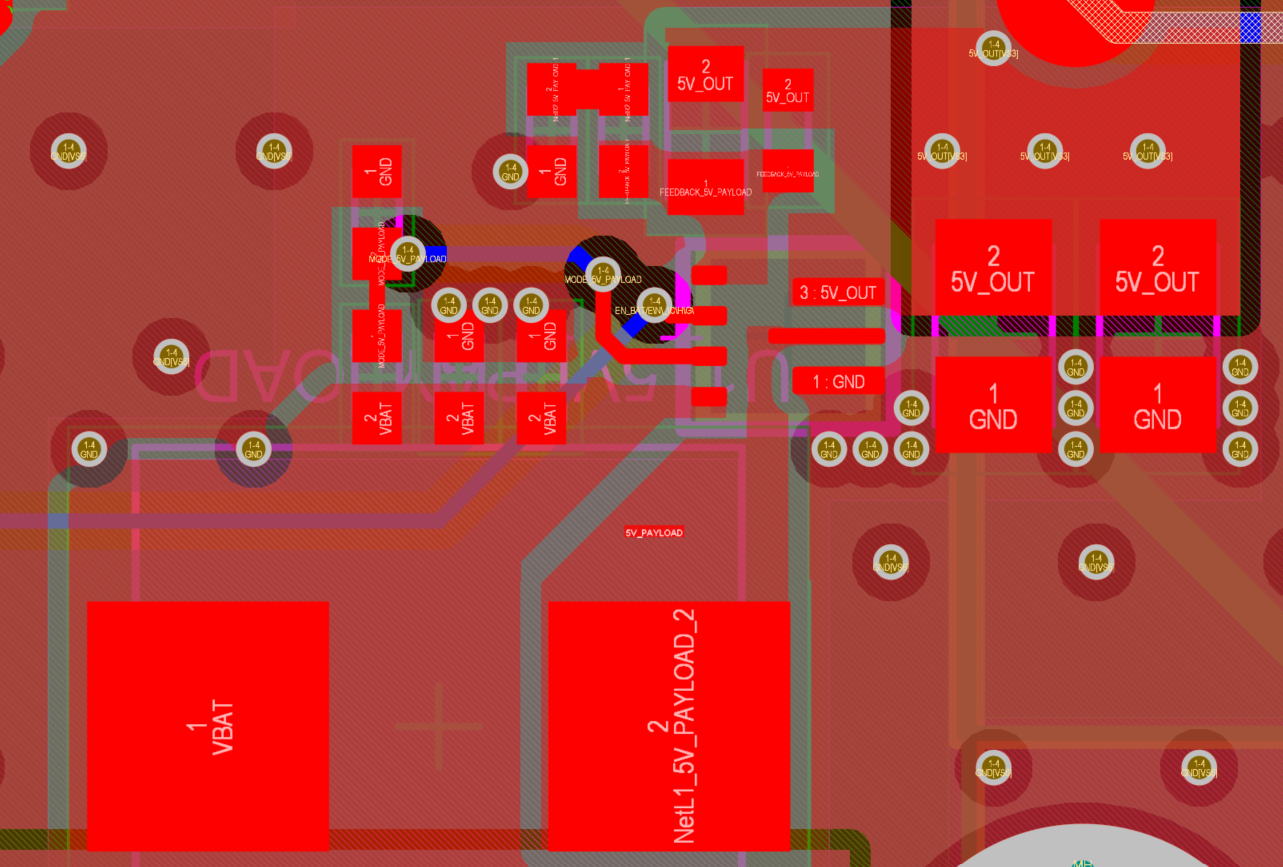
\includegraphics[width=\linewidth]{images/TPS61022-pcb-layout.svg.png}
    \caption{PCB layout implemented.}
  \end{subfigure}
  \caption{Layout of TPS61022 implemented in EPS.}
  \label{fig:TPS61022-layout}
\end{figure}

The \SI{3.3}{\volt} regulator was implemented from the reference design. The two ceramic capacitors were placed close to the regulator inputs and outputs to minimise noise. The output of the regulator was connected to the internal \SI{3.3}{\volt} power plane through multiple vias.

\begin{figure}[H]
  \centering
  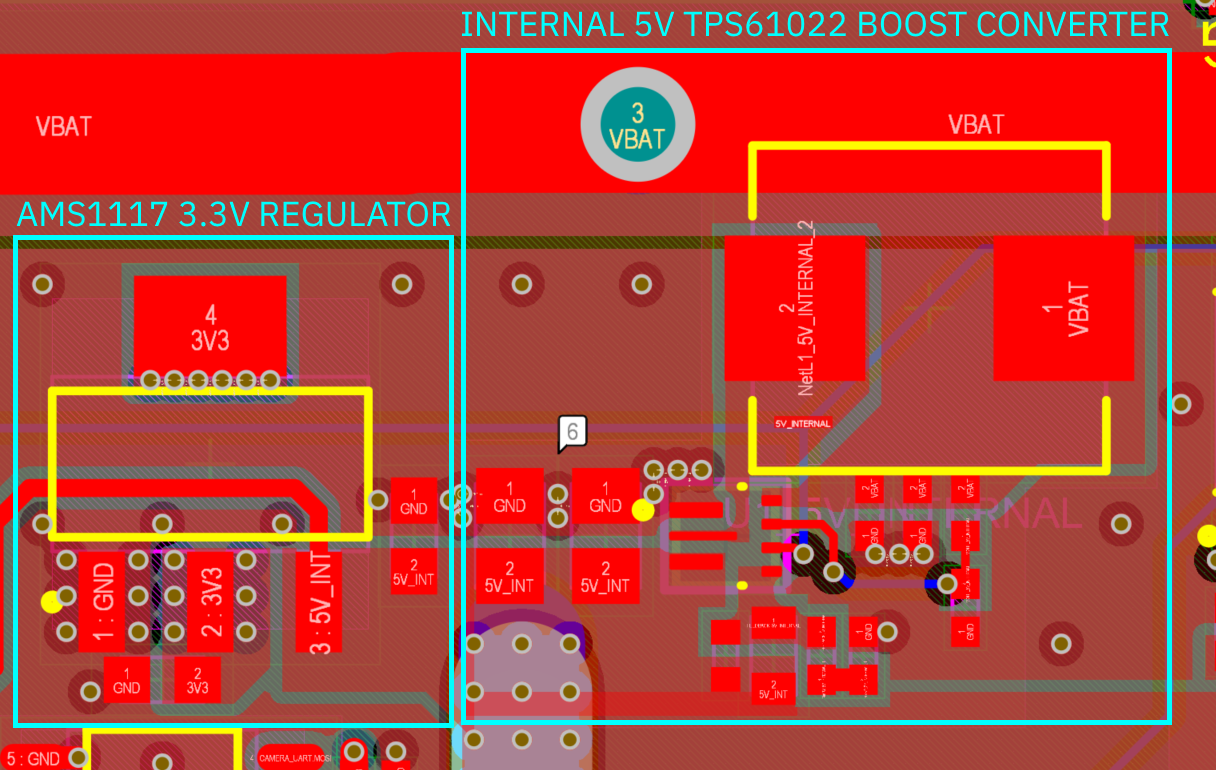
\includegraphics[width=\linewidth]{images/internal-power-supply.png}
  \caption{PCB layout of internal power conditioning, includes the layout of the AMS1117 regulator and another instantiation of the TPS61022 layout.}
  \label{fig:internal-power-supply}
\end{figure}

\section{Onboard Data Handling (OBDH)}

A first revision of the DAQ used an STM32L476 microcontroller, which had similar peripherals, including UART, {\iic} and SPI, however as a microcontroller it did not have an operating system, nor significant storage. Storage was provided in the form of a \SI{4}{\giga\byte} embedded multimedia card (eMMC) chip, which was chosen since it is directly soldered to the PCB and was more resistant to vibration than a micro SD card connector.
% TODO: talk about other cubesats using the stm32 platform?

Due to the issues encountered with the first revision and due to the time constraints, the second revision uses a Raspberry Pi Zero W v1.3 (referred to as "Pi Zero"). This was a development board which integrates the BCM2835 Broadcom system on chip (SoC), \SI{512}{\mega\byte} of RAM and contained a micro-SD card slot, USB interface and peripherals such as UART, {\iic} and SPI \cite{upton2016raspberry}. This board was chosen due to its small form-factor compared to larger Raspberry Pis, simplicity of integration compared to the Raspberry Pi compute modules and low cost. The Raspberry Pi platform has been used in low-cost low Earth orbit (LEO) CubeSat applications \cite{guertin2022raspberry}. It was predicted that in polar orbits that the Pi Zero has a lifespan of 5 years \cite{guertin2022raspberry}, which was adequate for this project since the POEM would cease to maintain its orbit after several months. The thermal performance of a Raspberry Pi Zero W was adequate for space applications \cite{guertin2022raspberry}. While a Raspberry Pi Zero 2W was initially selected, which would have had higher performance compared to the Zero v1.3, it was not possible to acquire one due to supply chain issues.

Typically, a Raspberry Pi runs the Raspbian operating system (OS), which is a Debian fork \cite{upton2016raspberry}. Compared to developing for a microcontroller, an OS is easier to develop for as it allows the use of standard Linux utilities for interacting with the system, including \texttt{ssh} for remote control, and having each DAQ task in a separate process with separated memory makes debugging easier. This ease of development was required to meet the time constraint of the project. %TODO: Citation`'

Due to limitations of the BCM2835 SoC only one hardware UART was available \cite{upton2016raspberry}, but more are required for receiving data from GNSS receivers. Receiving data through a software implementation of UART is not ideal since it uses a large amount of CPU resources and is prone to missing bits especially on the non realtime OS of the Raspberry Pi which severely limits its usable baud rate. The XR20M1172 dual hardware UART to add more UART ports to the Raspberry Pi through the SPI bus. This UART has a 64-byte first-in first-out (FIFO) buffer and interrupts, which eliminates the need for expensive polling, and has a maximum data rate of \SI{16}{\mega\bit\per\second} \cite{maxlinear2022xr20m1172}, which was more than adequate for GNSS data which has a maximum baud rate of only \SI{38400}{\baud}. This UART has a temperature range of \SIrange{-40}{85}{\degreeCelsius}, allowing it to survive temperature testing.

\subsection{Camera Communications Interface and Camera Data Downlink}

\subsubsection{Connector}
The final design of the camera payload interface used a DE-9 connector. This was chosen due to its low cost and ability to be secured using bolts instead of by friction alone. The pinout of the connector is shown in figure \ref{fig:de-9-connector}. The RS-485, power and ground lines were duplicated for redundancy.

\begin{figure}[H]
  \centering
  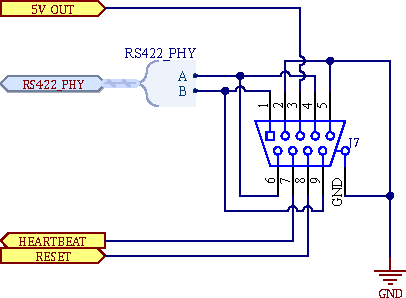
\includegraphics[width=\linewidth]{images/de-9-connector.pdf}
  \caption{Pinout of DE-9 connector.}
  \label{fig:de-9-connector}
\end{figure}

A female DE-9 connector was soldered to the DAQ, a male solder cup DE-9 terminal was soldered to 22 AWG copper cable to form the wire harness to the camera payload.

\subsubsection{RS-485 Receiver}
The SP3485EN-L/TR RS-485 transceiver was used to convert the RS-485 signalling to single-ended UART. The transceiver was fixed in receive mode since there is no way for the POEM to send data to the payload. The transceiver contains a \SI{120}{\ohm} d.c. termination as this was the end of the RS-485 bus, the resistor is sized to handle the power dissipation of a \SI{5}{\volt} RS-485 bus. The receiver contains a PSM712-LF-T7 transient voltage suppressor (TVS) diode array, which was designed to prevent the transceiver from being damaged by electrostatic discharge (ESD) due to manual handling of the connector.

\subsubsection{Transport Layer}
The camera payload communicates with the DAQ through UART at the transport layer. The settings in table \ref{tabl:uart-settings} were agreed upon and are used on both the payload and DAQ sides:
\begin{table}[H]
  \centering
  \begin{tabular}{|c|c|L{0.6\linewidth}|}
    \hline
    \textbf{Attribute} & \textbf{Value}    & \textbf{Note}                                                                                                                                                                                           \\
    \hline
    Speed              & \SI{57600}{\baud} & This is significantly more than the \SI{5000}{\baud} connection provided by POEM, but the drone and HPR tests have limited time and require faster transmission to receive any picture during the test. \\\hline
    Data bits          & 8                 &                                                                                                                                                                                                         \\\hline
    Stop bits          & 1                 &                                                                                                                                                                                                         \\\hline
    Parity             & None              &                                                                                                                                                                                                         \\\hline
    Flow control       & None              & This is a one-way connection, so software flow control is not possible.                                                                                                                                 \\\hline
  \end{tabular}
  \caption{UART settings.}
  \label{tabl:uart-settings}
\end{table}


\subsubsection{Presentation Layer}

Several simple formats are used in the presentation layer for this project. The data stream may contain either messages or image data.

Messages consist of a header, the message data of a variable length and an end of message marker as shown in figure \ref{fig:message-bytefield}. The header is sufficiently long and unique that it should not appear in the image data stream. Since messages are not often transmitted, this overhead is acceptable.

\begin{figure}[H]
  \centering
  \begin{bytefield}[bitwidth=0.4em]{80}
    \bitheader{0,79} \\
    \wordbox[lrt]{2}{Start of message: \texttt{\string{0x59,0x43,0x05,0x94,0x30,0x59,0x43,0x05,0x94,0x30\string}}} \\
    \wordbox[lrt]{1}{Message data, variable length} \\
    \skippedwords \\
    \wordbox[lrb]{1}{} \\
    \wordbox[lrb]{2}{End of message: \texttt{\string{0x59,0x43,0x05,0x94,0x30,0x59,0x43,0x05,0x94,0x30\string}}}
  \end{bytefield}
  \caption{Message structure.}
  \label{fig:message-bytefield}
\end{figure}

A chunk protocol is used for the transmission of images in the final design. A preliminary design simply sequentially transmitted each byte of the image, which was adequate when the radio was placed close to each other ($>\SI{10}{\meter}$). However, when testing past this range and at any significant distance, the errors caused the received image to become unrecognisable. The type of error observed consists of contiguous bytes being lost occasionally, rather than frequent corruption of individual bytes as shown in \ref{fig:image-sheds-error-demo}.

\begin{figure}[H]
  \centering
  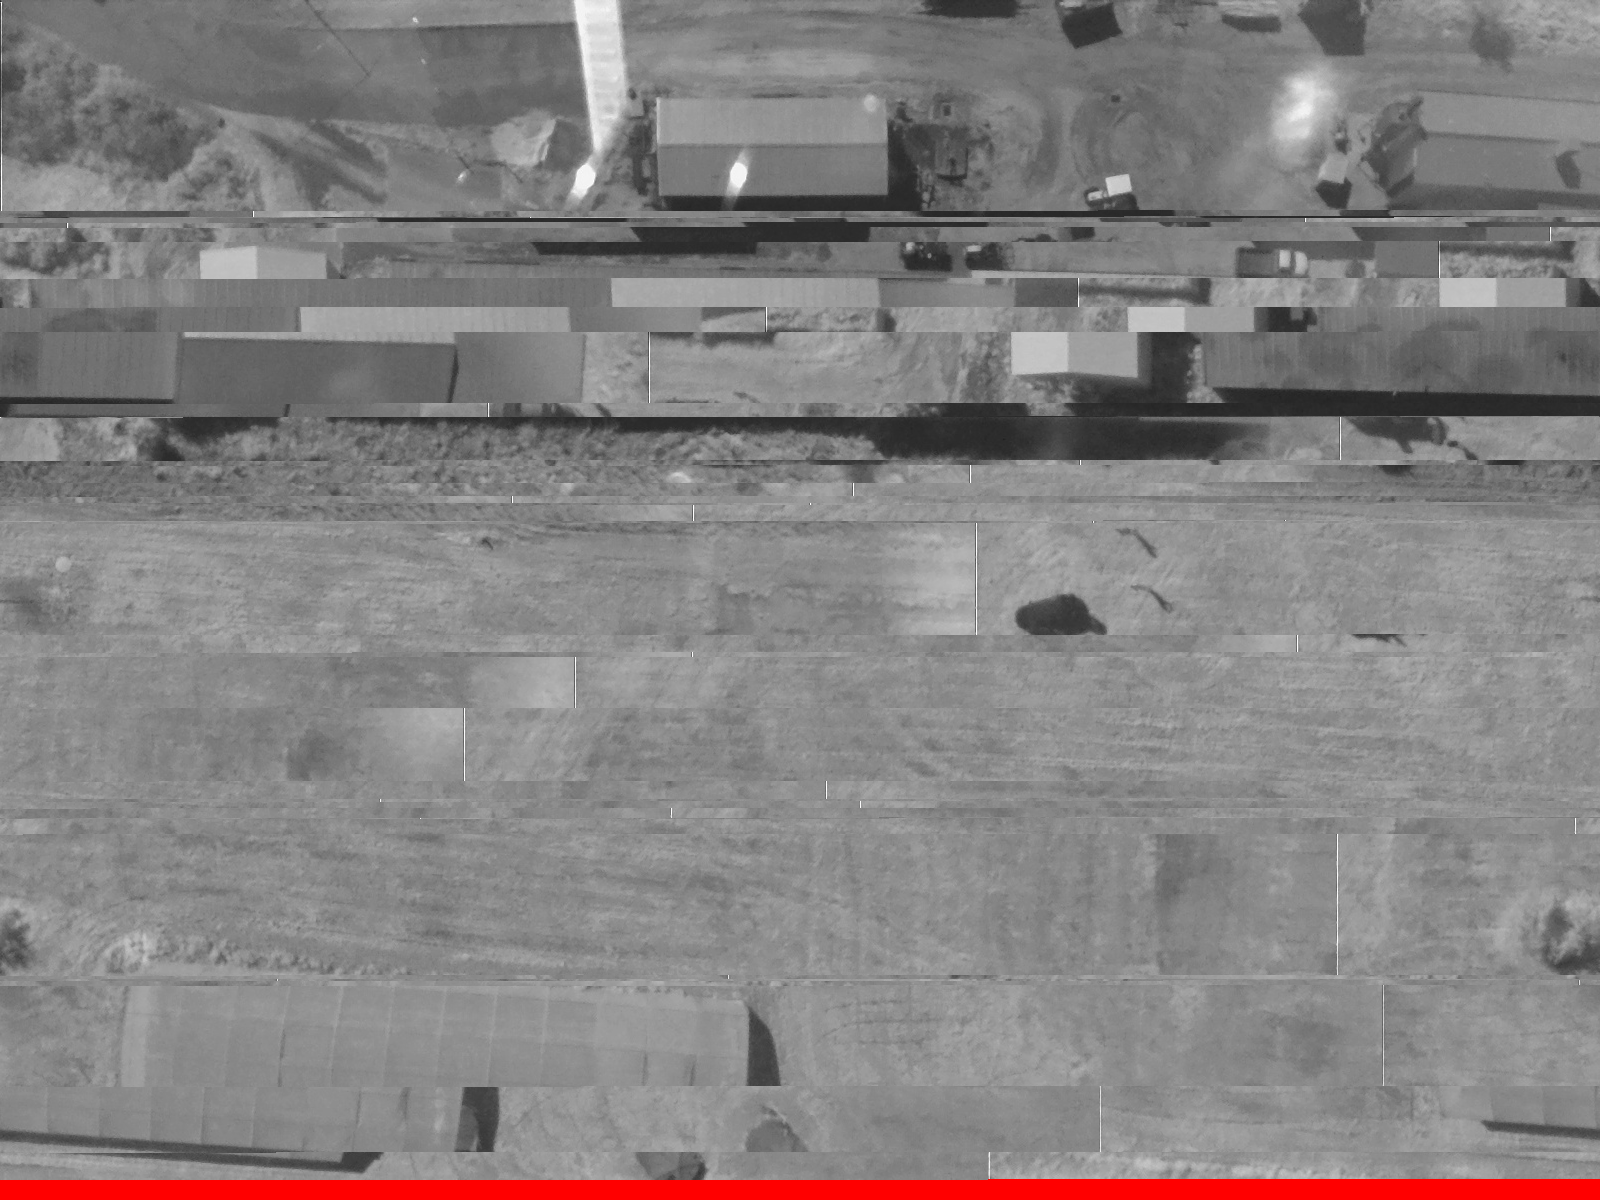
\includegraphics[width=\linewidth]{images/results/sheds_naive.png}
  \caption{Example of an image received with errors resulting in an unrecognisable image due to dropped bytes causing the image to shift at each error. Only a small proportion of the image is lost ($<3\%$), represented by red pixels at the bottom and contiguous sections of the received image are error-free.}
  \label{fig:image-sheds-error-demo}
\end{figure}

A chunk protocol was effective against this type of error while being simple to implement. It involved adding a header to signify the start of a chunk, followed by the chunk number and 400 bytes of pixel data as shown in \ref{fig:image-chunk-bytefield}. A \SI{1600x1200}{} pixel image where each pixel is represented by one byte required 4800 chunks to be sent in this implementation. The number of bytes per chunk is a trade-off between pixels lost per error and effective data rate.

A start of chunk marker of \texttt{\string{0x00, 0xFF, 0x00, 0xFF\string}} was chosen since the image data being transmitted are raw pixels, and it was unlikely for the image to contain pixels that are full or zero intensity, and even more unlikely for them to be adjacent to each other.

When an error occurs causing a string of bytes to be dropped, it causes the next chunk to not be encountered after 400 bytes. When this error occurs, the receiver searches for the next occurrence of the header and restarts receiving from that point. The chunks which were skipped have their pixels filled in the received image to prevent the error causing the image to become unrecognisable.

The end of an image is signified by the ASCII string "EOFEOFEOFEOF". The start of chunk of the next image immediately starts after this string.

\begin{figure}[H]
  \centering
  \begin{bytefield}[bitwidth=0.33em]{112}
    \bitheader{0,31,47,95} \\
    \bitbox{32}{Start of chunk} & \bitbox{16}{ID 0} & \bitbox[tr]{64}{}\\
    \wordbox[lr]{1}{Greyscale pixel data, 400 bytes, 1 byte per pixel.} \\
    \skippedwords \\
    \wordbox[lrb]{1}{} \\
    \wordbox[]{1}{$\vdots$} \\[1ex]
    \bitbox{32}{Start of chunk} & \bitbox{16}{ID 4799} & \bitbox[tr]{64}{}\\
    \wordbox[lr]{1}{Greyscale pixel data, 400 bytes, 1 byte per pixel.} \\
    \skippedwords \\
    \wordbox[lrb]{1}{} \\
    \bitbox[lrb]{96}{End of image marker \texttt{"EOFEOFEOFEOF"}}
  \end{bytefield}
  \caption{Image chunk protocol.}
  \label{fig:image-chunk-bytefield}
\end{figure}

\subsubsection{Radio Downlink}
The RFD900x radio transceiver was chosen to emulate the POEM radio service. This transceiver uses the 915 MHz industrial, scientific and medical (ISM) band and transmits with a maximum power of \SI{1}{\watt} using a frequency hopping spread spectrum (FHSS) technique \cite{rfdesign2020rfd900x}. Data rates from \SI{12}{\kilo\bit\per\second} to \SI{224}{\kilo\bit\per\second} are available with the default firmware \cite{rfdesign2020rfd900x}. The RFD900x uses a UART to transmit and receive data \cite{rfdesign2020rfd900x}.

The RFD900x satisfies several constraints. It reduced the time to test since it uses the ISM band, which can be used by anyone provided they follow the Low Interference Potential Devices (LIPD) Class License legislation. The use of FHSS allowed the RFD900x to transmit at the maximum power of \SI{1}{\watt} that is allowable by the class license under the frequency hopping transmitters section \cite{australia2015radiocommunications}.

Distances of \SI{40}{\kilo\metre} line-of-sight were possible using the RFD900x \cite{rfdesign2020rfd900x}, which was far greater than the maximum distance achievable with the rocket and drone tests. The maximum drone test scheduled had an altitude of \SI{500}{\metre}, and the rocket was intended to fly to \SI{10000}{\feet} (\SI{3}{\kilo\metre}).

The radio transceiver had a temperature range of \SIrange{-40}{85}{\degreeCelsius}, which satisfied the range of temperatures required to pass the temperature testing \cite{rfdesign2020rfd900x}.

\subsubsection{Camera Communications and Downlink Software}

A Python script was developed for the DAQ which:

\begin{enumerate}
  \item Opens the serial port \texttt{/dev/serial0} with the settings described in table \ref{tabl:uart-settings}.
  \item Create and open a log file with a unique filename to dump the received bytes from the camera payload.
  \item Periodically read a block of 2048 from the UART receive buffer and write the block to the file and UART output.
  \item Every 3 seconds write a message to the UART output containing the current system time, the script's uptime and the number of UART errors.
\end{enumerate}

This Python script is managed by a \texttt{systemd} service which reboots the script if it crashes.

The ground station is a laptop running Windows with an RFD900x connected to it over USB serial. There are two Python scripts on the laptop, the first saves the data from the radio to a file and prints any messages to the console.

\begin{enumerate}
  \item Opens a serial port to the RFD900x with the UART settings of the ground RFD900x.
  \item Create and open a log file to store the received bytes from the radio.
  \item Periodically:
        \subitem Read the bytes in the serial buffer,
        \subitem Save the bytes to the log file,
        \subitem Find any start of message mark, and if encountered print all bytes until the end of message mark is received
\end{enumerate}

A second script periodically reads the latest log file and splits it into images.

\begin{enumerate}
  \item Allocate a \texttt{bytearray} for a full \SI{1600x1200}{} pixel image.
  \item Allocate a \SI{1600x1200}{} \texttt{bytearray} where each byte is the state of each pixel (received or missing).
  \item Read the whole file and strip all messages (bytes enclosed by the start and end of message markers).
  \item Then find the indices of the end of image makers and split the file into several bytearrays, one for each image.
  \item For each image bytearray:
        \subitem Find the next start of chunk
        \subitem Extract the chunk ID from the next two bytes.
        \subitem Extract image bytes starting from after the chunk ID to either the next header index, or the end of file if this doesn't exist.
        \subitem Add all bytes to the image byte array, starting at index \texttt{ID * 400} and set the state of the added pixels to "received".
        \subitem Repeat until the image array is full or there are no more bytes left in the image bytearray.
\end{enumerate}

\paragraph{Results}

This system was tested in the drone test at a distance of \SI{120}{\meter} line of sight. The image received is shown in \ref{fig:image-blocking-example} with comparison to an image received without blocking:

\begin{figure}[H]
  \begin{subfigure}{0.495\textwidth}
    \centering
    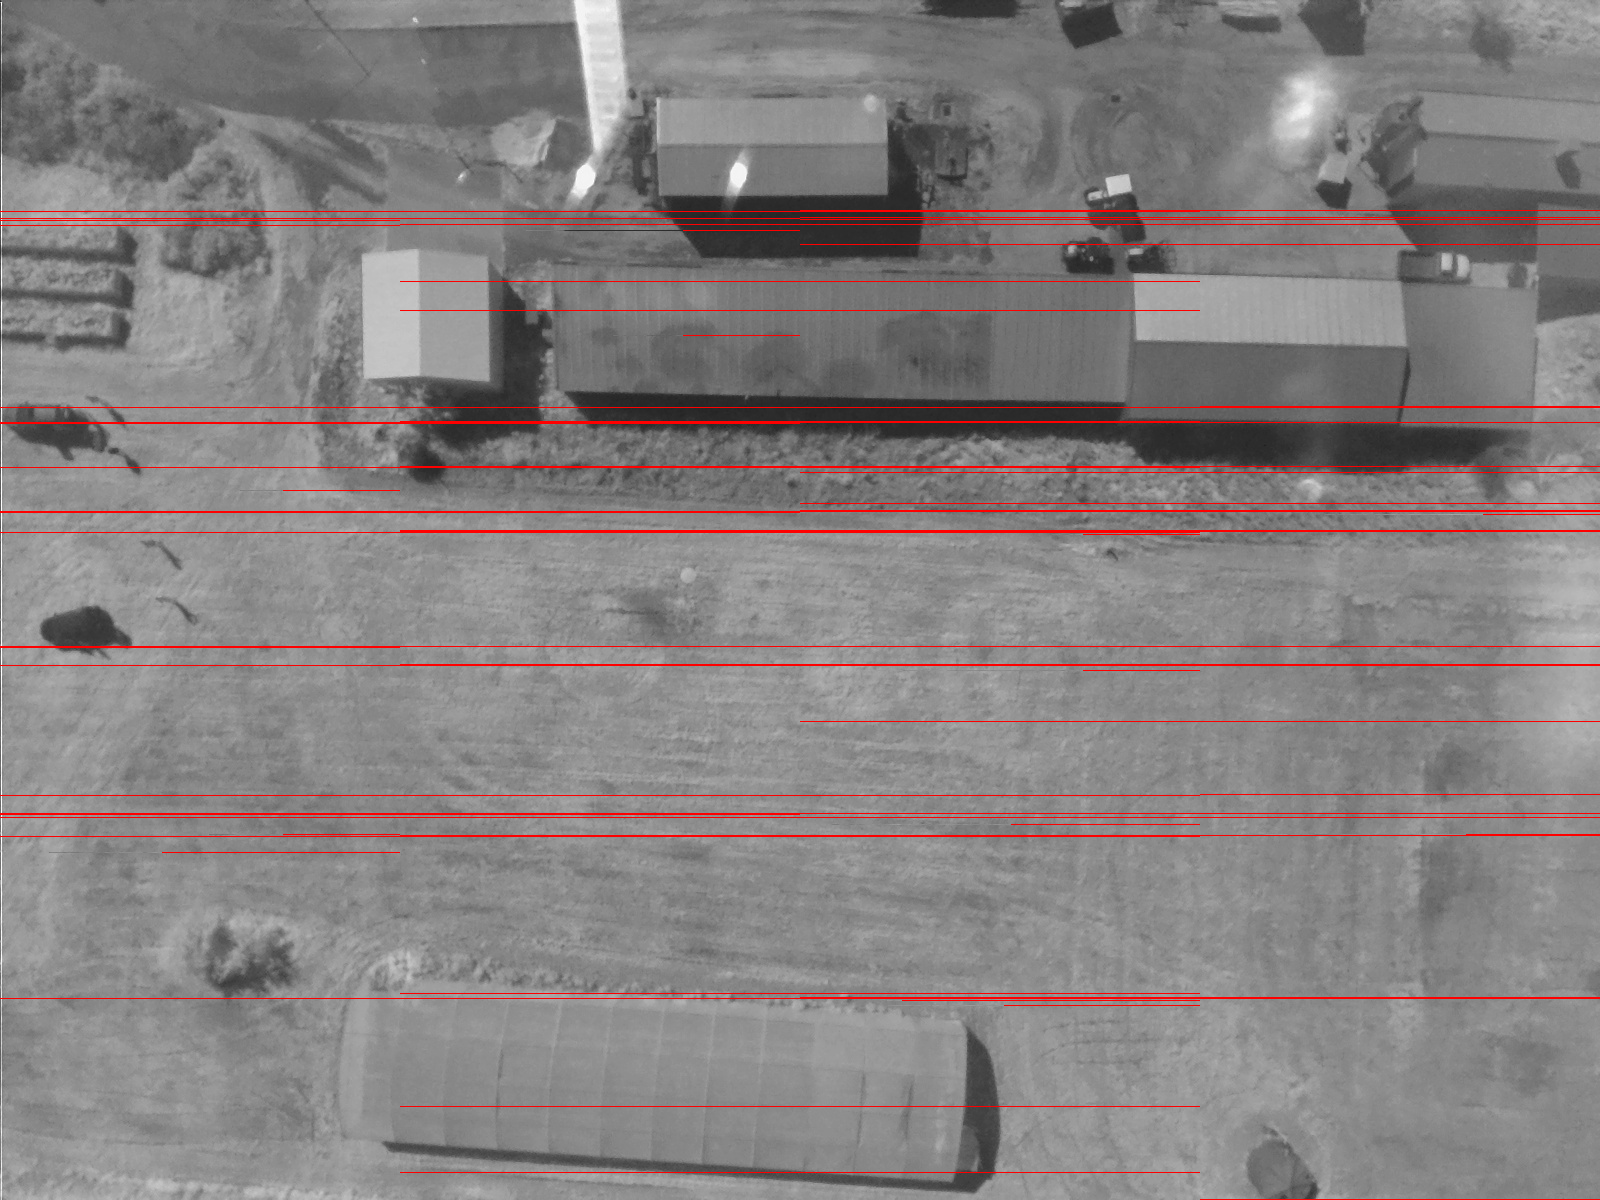
\includegraphics[width=\linewidth]{images/results/sheds.png}
    \caption{}
  \end{subfigure}
  \begin{subfigure}{0.495\textwidth}
    \centering
    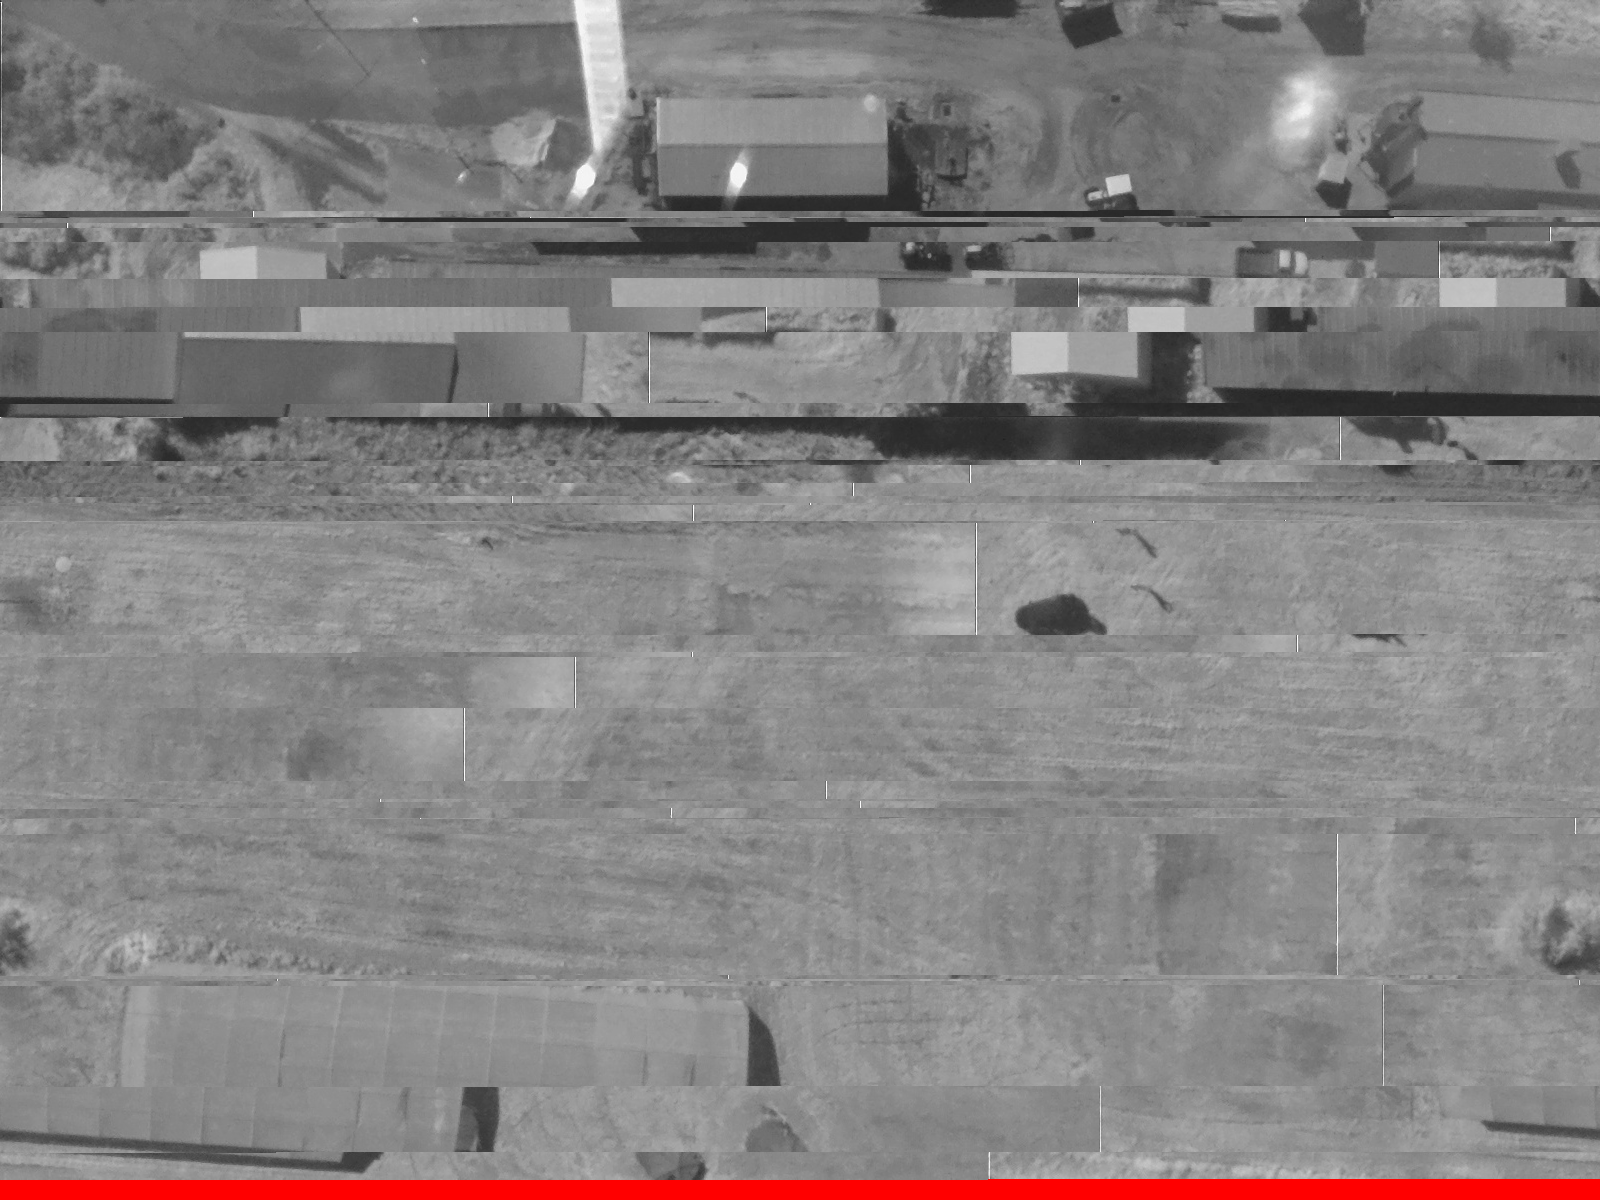
\includegraphics[width=\linewidth]{images/results/sheds_naive.png}
    \caption{}
  \end{subfigure}
  \caption{Comparison of two image reception techniques. Image (a) used the blocking protocol with a block size of 400 pixels. Image (b) is an example of what the image would look like without the image blocking.}
  \label{fig:image-blocking-example}
\end{figure}

\subsection{Accelerometer Data Acquisition System}
\subsubsection{Accelerometer Selection}

Two accelerometers MEMS were chosen, the ADXL\-375 and LSM6\-DSOX.

The STMicroelectronics LSM6\-DSOX is a MEMS inertial measurement unit (IMU) which has a $\pm\SI{16}{\gacc}$ accelerometer and $\pm\SI{2000}{\milli\degree\per\second}$ gyroscope, both with a sampling rate of \SI{6666}{\kilo\hertz}. This accelerometer was used to characterise the random vibration spectrum of launch due to its high sampling rate.

Due to the low full-scale of the LSM6\-DSOX of only $\pm\SI{16}{\gacc}$, the ADXL\-375 was chosen to characterise the shock response of the payload to pyroshock due to its significantly higher full-scale range of $\pm\SI{200}{\gacc}$.

Based on the accelerometer specifications, these accelerometers satisfy the requirements outlined in table \ref{tabl:acc-requirements}.

\subsubsection{Accelerometer PCB}

The accelerometer PCB (shown in figure \ref{fig:accelerometers-pcb}) contained both the ADXL\-375 and LSM6\-DSOX accelerometers and mounted them to the chassis.

To maximise the resonant frequency of the assembly, the PCB was mounted on its flat side to the chassis and was fixed with four steel M3 bolts on each corner. Additionally, the dimensions of the PCB was minimised to \SI{22x22}{\milli\metre}, which was the minimum dimension that can fit all components. Maximising the resonant frequency past the sampling frequency would minimise distortion of the response. The PCB is depicted in figure \ref{fig:accelerometers-pcb}.

The PCB exposed one interrupt and chip select pin for each accelerometer, an SPI connection and \SI{3.3}{\volt} power bus.

\begin{figure}[H]
  \centering
  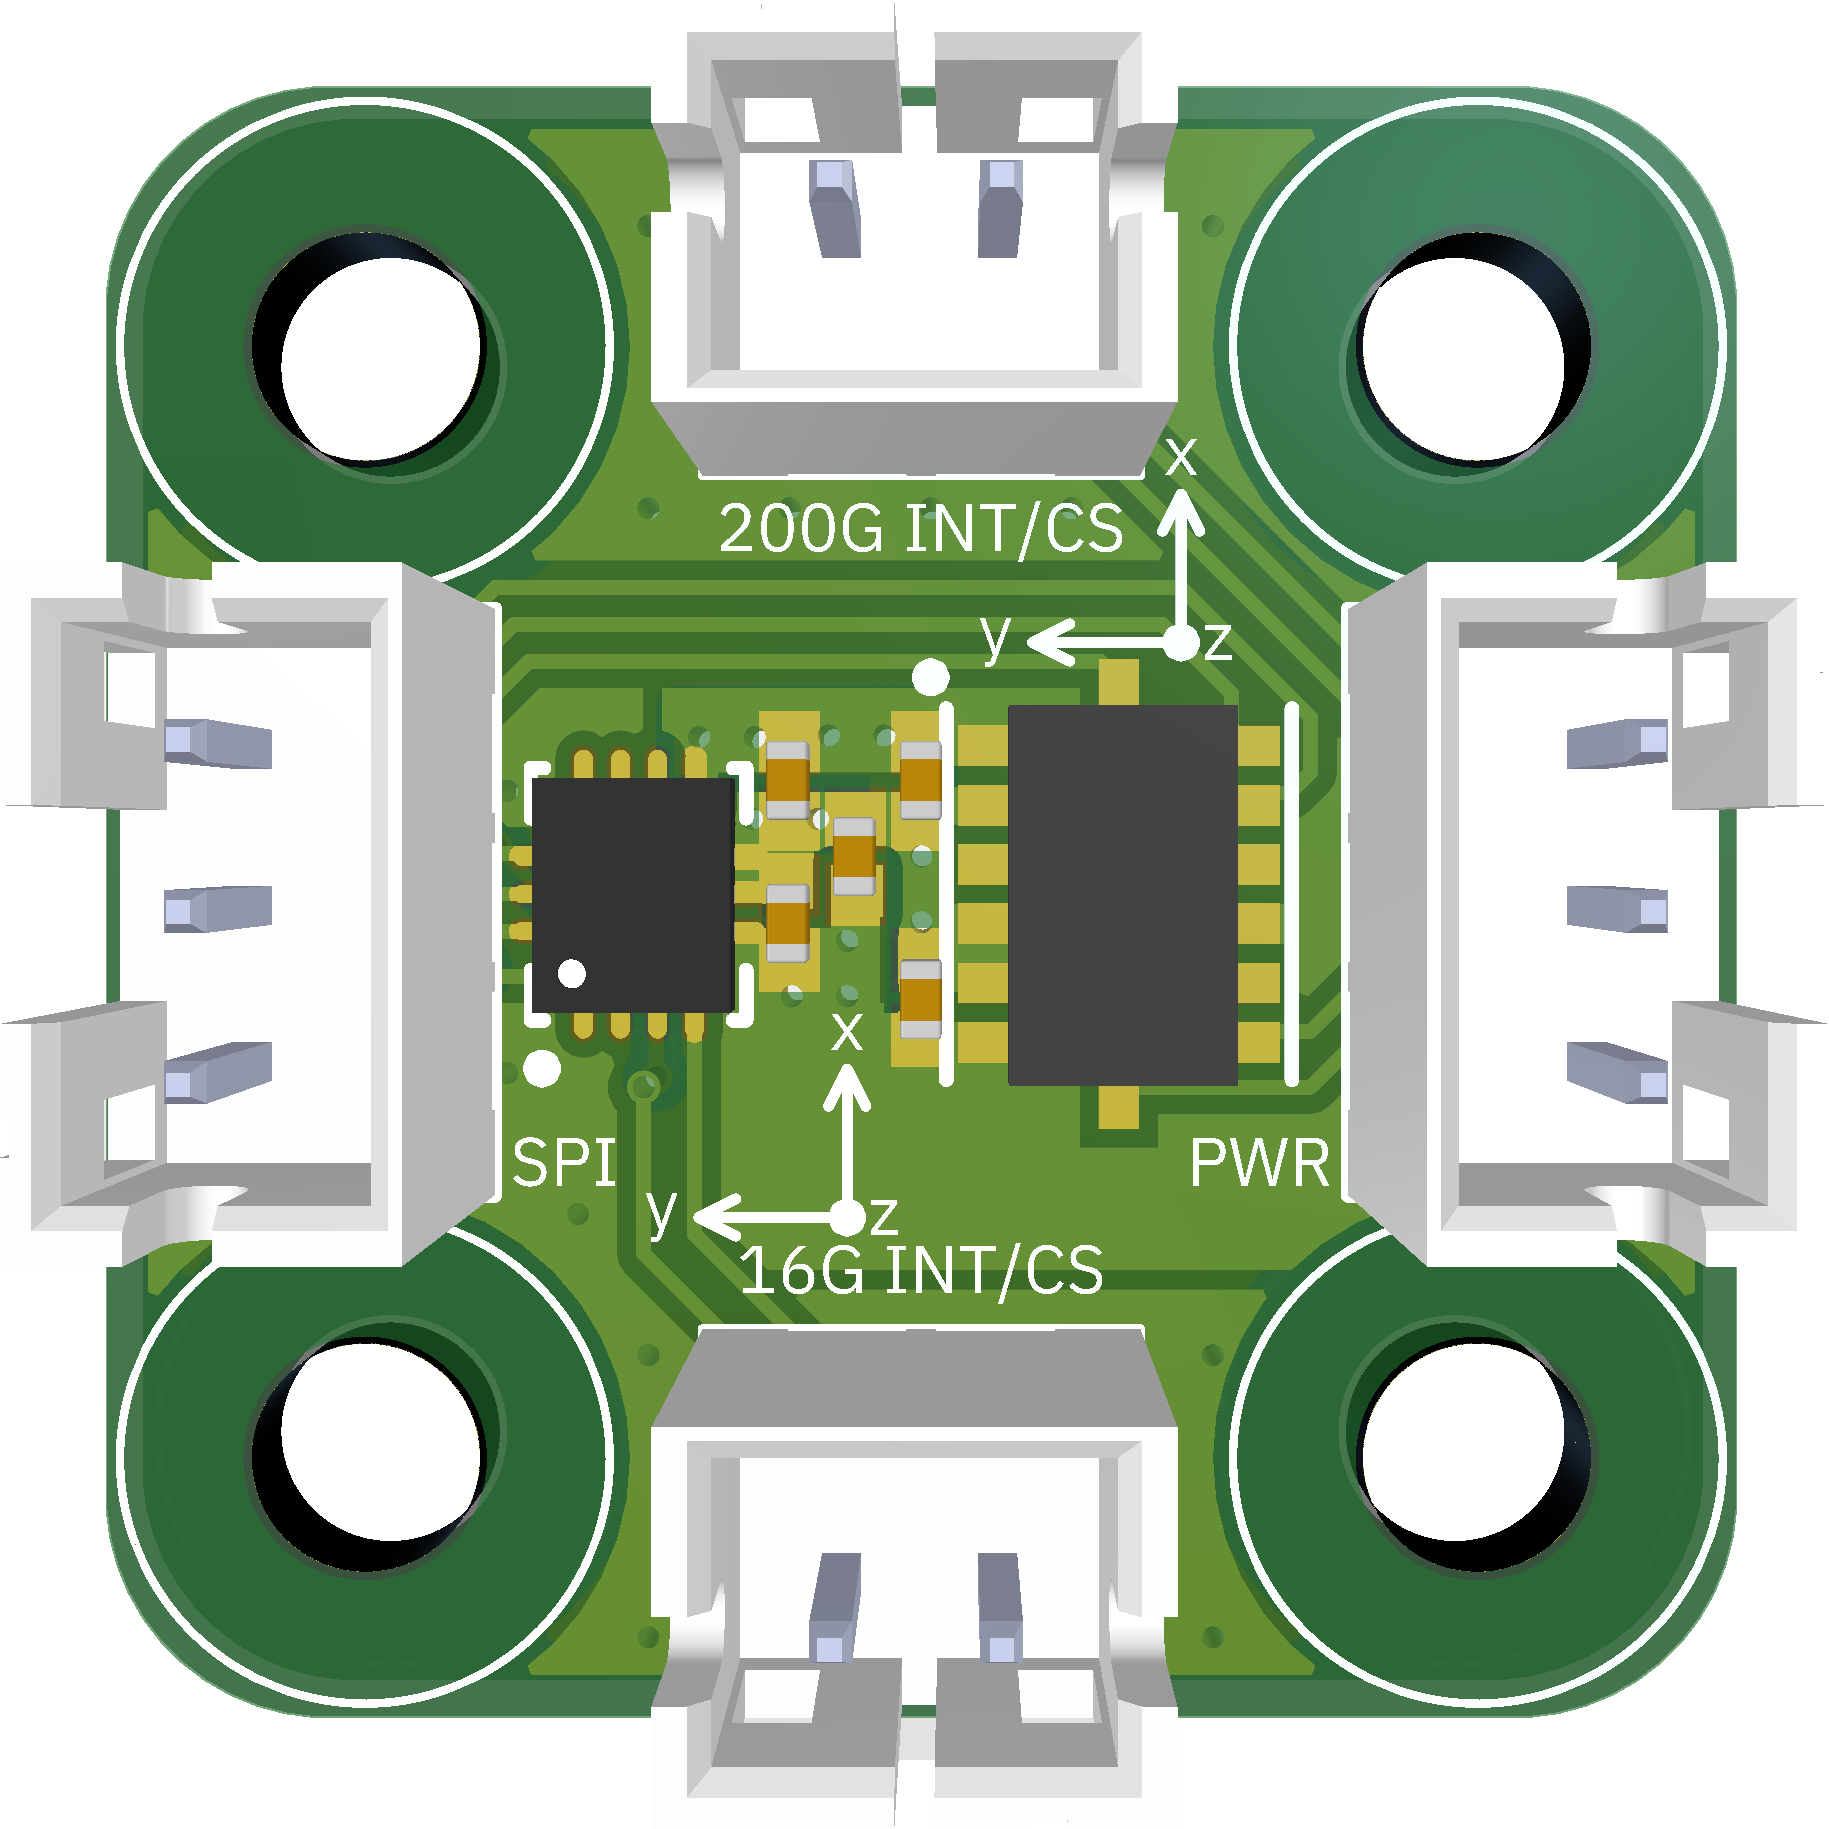
\includegraphics[width=0.5\linewidth]{images/Accelerometers_PCB.png}
  \caption{Accelerometer PCB.}
  \label{fig:accelerometers-pcb}
\end{figure}

\subsubsection{Connection to DAQ}

The accelerometers were connected to the DAQ using the \texttt{SPI0} bus of the Pi Zero. The chip select (\textoverline{CS}) and interrupt (INT) pins were connected to GPIOs and handled by software, therefore it was not necessary to only use the hardware SPI chip select/chip enable (CE) pins for all chip selects. This is depicted in figure \ref{fig:accelerometers-sch-block}. Although SPI requires more wiring, in the case of these sensors SPI has a higher clock speed compared to {\iic}. For example, the LSM6DSO has supports the {\iic} Fast Mode+ extension (FM+) which gives the {\iic} bus a maximum clock rate of \SI{1}{\mega\hertz}, but the SPI has a maximum clock speed of \SI{10}{\mega\hertz} which is higher. SPI also has higher data rate for a given frequency than {\iic} since {\iic} adds additional flow control bits such as start, stop and acknowledgement bits.

This SPI bus was dedicated for only accelerometers to maximise the number of accelerometers connected, and was not shared with non-accelerometer peripherals. Two accelerometers were used as redundancy.

\begin{figure}[H]
  \centering
  \includesvg[width=0.8\linewidth]{images/accelerometer_daq.svg}
  \caption{Block diagram of accelerometers and Pi Zero data acquisition system.}
  \label{fig:accelerometers-sch-block}
\end{figure}

\begin{figure}[H]
  \begin{subfigure}{0.495\textwidth}
    \centering
    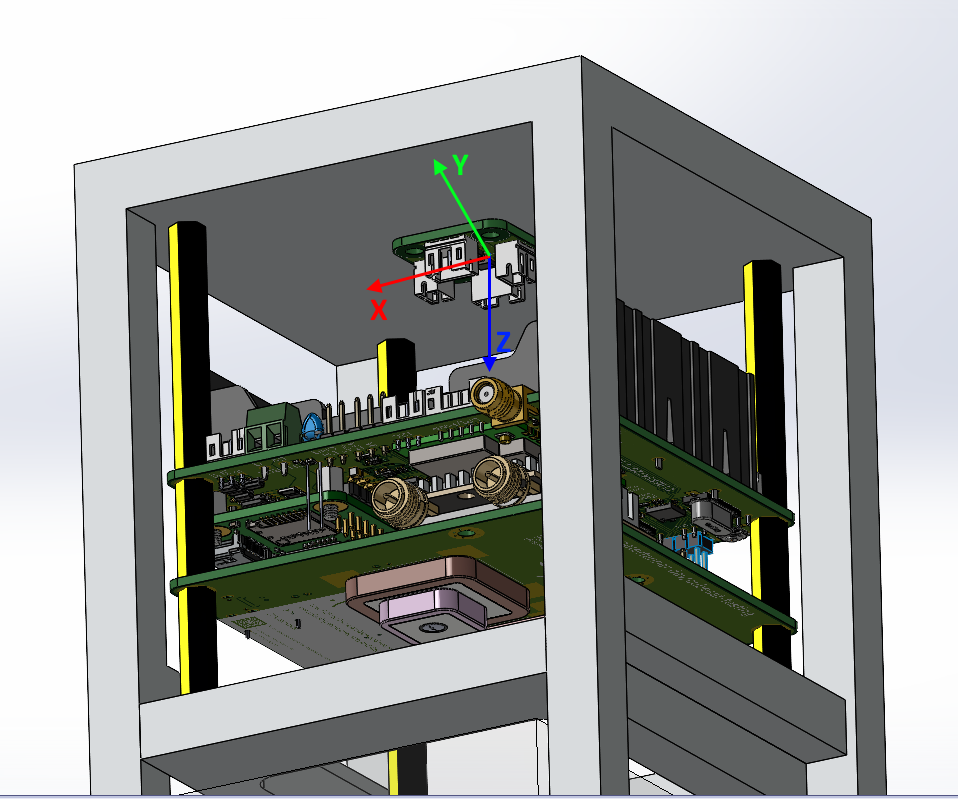
\includegraphics[width=\linewidth]{images/results/top_accelerometer.png}
    \caption{Top accelerometer}
  \end{subfigure}
  \begin{subfigure}{0.495\textwidth}
    \centering
    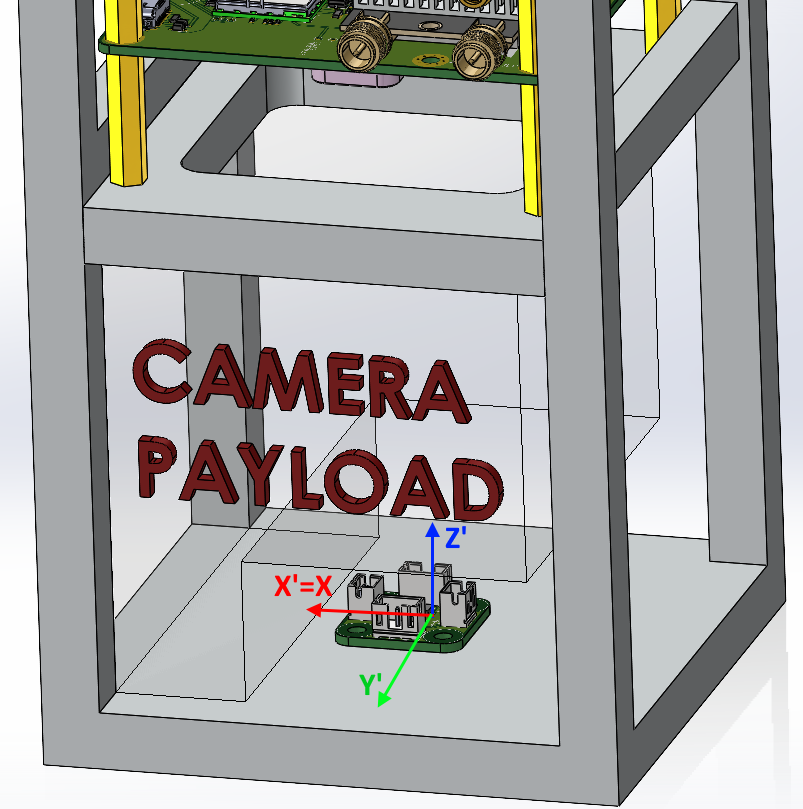
\includegraphics[width=\linewidth]{images/results/bot_accelerometer.png}
    \caption{Bottom accelerometer.}
  \end{subfigure}
  \caption{Mounting positions of accelerometers on the CubeSat chassis. The top and bottom accelerometer share a common $x$ axis but have opposite $y$ and $z$ axes.}
  \label{fig:accelerometer-mounting}
\end{figure}

\subsubsection{LSM6\-DSOX Software}
A C program was written to read values from the LSM6\-DSOX, package them into a binary flat file format and store them to disk. A C program was required since preliminary tests with a Python script with the same functionality resulted in 100\% of the CPU being used to read from one accelerometer.

The \texttt{lsm6dso-pid} platform independent (PID) library was used to provide simple access to the registers of the accelerometer \cite{stmicroelectronics_lsm6dsox_pid}, in combination with WiringPi which provided bindings to GPIO, SPI and other peripherals on the Pi \cite{wiringpi-github}.

To maximise sampling rate and minimise CPU usage, the accelerometer is operated using the FIFO and interrupt features.

Samples from the accelerometer were stored in binary flat file format, consisting of the \texttt{struct datapoint} for each 3-axis sample. A header of \texttt{0x59} was used which signifies the start of a sample. The type field was set to either 1 for accelerometer samples or 2 for gyroscope samples.

\begin{lstlisting}[language=C]
struct datapoint
{
    char header;
    char type;
    float x;
    float y;
    float z;
};
\end{lstlisting}

To improve reliability, the LSM6\-DSOX program contains a watchdog, implemented using a POSIX timer, which restarts and re-initialises the accelerometer if no samples have been received for \SI{1}{\second}. The process is managed by a \texttt{systemd} service which initialises the program on system boot and restarts the program if it crashes.

The following is a description of the program

\begin{enumerate}
  \item Read the first argument, which describes the sensor that the process will manage (1 or 2), and open the appropriate SPI bus using WiringPi.
  \item Open a new unique binary file to store the samples to.
  \item Create a watchdog POSIX timer and debug printing POSIX timer.
  \item Attach the FIFO read interrupt handler on the interrupt pin.
  \item Initialise the LSM6\-DSOX by issuing the following commands:
  \item Ensure the \texttt{WHO\_AM\_I} register matches the expected value,
  \item Software reset the device,
  \item Wait for the device to be reset,
  \item Disable the I\textsuperscript{3}C interface,
  \item Enable block data update,
  \item Set the scale for the accelerometer to \SI{16}{\gacc}, the maximum full scale possible,
  \item Set the sampling rate to \SI{6666}{\hertz} and the batching rate to \SI{12.5}{\hertz},
  \item Set the FIFO to continuous mode (old samples are automatically discarded),
  \item Set FIFO watermark level to 384 samples,
  \item Set interrupt pin 1 to pulse on FIFO watermark being reached (this results in a pulse being generated on the INT1 pin when a large amount of data is present in the FIFO to be read, resulting in the interrupt handler being triggered.),
\end{enumerate}

The interrupt handler has the following functionality and is based off sample code from the LSM6\-DSOX PID library \cite{stmicroelectronics_lsm6dsox_pid}:

\begin{enumerate}
  \item Immediately reset the watchdog timer to 1 second (to prevent it triggering since a read is started)
  \item Read the number of samples in the FIFO. For each sample:
  \item Read the sample's tag and if it is accelerometer data then read the sample from the FIFO into a 6-byte array
  \item Convert each of the three axes (represented by two byte words) to \SI{}{\milli\gacc}.
  \item Store the reading in a struct with the correct header and type and write to the log file.
  \item For debug reasons, print the current sample every 3332 samples (every half second).
\end{enumerate}

\subsubsection{Unpacking Data for Data Analysis}

The accelerometer binary files were read on a PC using a Python script which uses the \texttt{struct} library to unpack the file and converted it to a traditional comma-separated values (CSV) file.

\subsubsection{ADXL375 Software}

A separate process was created for the ADXL375, however the code uses the same procedure for the LSM6DSOX. The only changes are the initialisation process, where it sets registers to put the accelerometer into \SI{200}{\gacc} full scale and \SI{1600}{\hertz} sampling rate, and changes in the watermark level. The addresses of the registered were changed for the ADXL375, but the high-level procedure is similar.

\subsection{GNSS Tracking}

The u-blox NEO-M9N was used for tracking \cite{ublox2023neo_m9n_datasheet}. This is a multi-GNSS receiver which is able to receive from multiple GNSS constellations simultaneously, which results in a faster acquisition time and greater interference immunity \cite{ublox2023neo_m9n_datasheet}. The receiver can report position with an accuracy of \SI{2.0}{\metre} (circular error probable), which is adequate for a HPR tracking application \cite{ublox2023neo_m9n_datasheet}. The NEO-M9N was used instead of other u-blox receivers due to its high navigation update rate of \SI{25}{\hertz} which is useful due to the high speed of a HPR flight \cite{ublox2023neo_m9n_datasheet}.

Since POEM provides the location of the CubeSat and due to the speed and altitude restriction of the NEO-M9N of \SI{500}{\metre\per\second} and \SI{80}{\kilo\metre} respectively, this receiver will not be present on the space launch and is only required for the HPR launch.

A differential GNSS (DGNSS) solution was considered and tested based on the u-blox ZED-F9P, however the drone test did not require the centimetre level precision of the ZED-F9P, so it was not used in the final design.

\chapter{Final Experiment Design for HPR Evaluation}

The design of the DAQ was a precursor for the experiment to compare HPR to shaker table testing. Note that the results of the HPR and shaker table tests will also be used for evaluating the DAQ in addition to the goal of evaluating the usefulness of HPR launches for qualifying CubeSats.

\section{High-Power Rocket Flight}

A custom rocket named \textit{UNO} was designed and built by another project member (Jamir Khan) from scratch, it had a height of 290 cm, diameter of $\SI{16.3}{\centi\metre}$ and a dry mass of $\SI{14.42}{\kilo\gram}$ without a motor. It was designed to fly with an M impulse class motor, however due to changes in United States export regulations it was not possible to obtain this motor in time, therefore it was only possible to launch with a K impulse class motor which has about 1/10th of the total impulse of the N motor as shown in table \ref{tabl:impulseclasses}. All analysis following this assume a K1100T motor.

\begin{table}[H]
  \centering
  \begin{tabular}{|c|c|}
    \hline
    Total impulse [$\SI{}{\newton\second}$] & Motor impulse class \\\hline
    160.01 - 320.00                         & H                   \\
    320.01 - 640.00                         & I                   \\
    640.01 - 1,280.00                       & J                   \\
    1,280.01 - 2,560.00                     & K                   \\
    2,560.01 - 5,120.00                     & L                   \\
    5,120.01 - 10,240.00                    & M                   \\
    10,240.01 - 20,560.00                   & N                   \\
    20,560.01 - 40,960.00                   & O                   \\
    40,960.01 - 81,920.00                   & P                   \\
    81,920.01 - 163,840.00                  & Q                   \\
    \hline
  \end{tabular}
  \caption{Rocket motor impulse classes \cite{nfpa2018}}
  \label{tabl:impulseclasses}
\end{table}

\begin{figure}[H]
  \includesvg[width=\textwidth]{images/honors-openrocket2.svg}
  \caption{OpenRocket diagram of \textit{UNO}.}
  \label{fig:openrocket}
\end{figure}

\subsection{Simulation}

The rocket was simulated using OpenRocket \cite{openrocket,niskanen2009}, an open-source simulator which can predict parameters such as stability and acceleration based on empirical methods which use the rocket's shape and basic environment parameters such as constant wind \cite{doi:10.1177/0954410017752730,niskanen2009}. OpenRocket was used to ensure the rocket design was stable throughout launch and flight, which was important to ensuring the CubeSat payload does not become damaged by this qualification method. However, as it used a simple empirical model of the flight, it was not designed to model the effect of the motor and aerodynamic forces on the vibration environment in the rocket. It also does not simulate pyroshock events, instead modelling parachute deployment events as simple changes in the aerodynamics of the rocket \cite{niskanen2009}.

\subsubsection{Flight Profile}

As shown in \ref{fig:openrocket-k-launch} the rocket was anticipated to reach an apogee of \SI{413}{\metre} at \SI{9.74}{\second} and a total flight time of \SI{30}{\second}.

\begin{figure}[H]
  \includesvg[width=0.8\textwidth]{images/k-ork-vertical.svg}
  \caption{Flight profile of \textit{UNO} using a K1100T motor. Simulated in OpenRocket.}
  \label{fig:openrocket-k-launch}
\end{figure}


\subsubsection{Stability}

As shown in figure \ref{fig:openrocket-k-stability}, the stability was above 2.0 calibres for the coast and launch phase, which was a general rule to ensure the rocket was stable and will not veer off course \cite{canepa2005modern}. The short moment of stability below 2.0 occurs when the rocket reaches apogee, which was not an issue since the parachutes are immediately deployed at this point.

\begin{figure}[H]
  \includesvg[width=0.8\textwidth]{images/k-ork-stability.svg}
  \caption{Stability of \textit{UNO} using a K1100T motor. Simulated in OpenRocket.}
  \label{fig:openrocket-k-stability}
\end{figure}

\subsubsection{Acceleration}

As stated, since OpenRocket does not model the vibration environment in the rocket and models the rocket as one solid body, only the acceleration of the whole rocket can be modelled. Pyroshock events are not modelled by OpenRocket. The launch phase lasts only \SI{1.6}{\second} and has a high average acceleration of \SI{5.77}{\gacc}, as shown in \ref{fig:openrocket-k-acceleration}. During the coast phase, the rocket is decelerated by gravity as expected and after parachute deployment the rocket only has a small deceleration force.

\begin{figure}[H]
  \centering
  \includesvg[width=0.8\textwidth]{images/k-ork-acceleration.svg}
  \includesvg[width=0.8\textwidth]{images/k-ork-acceleration-launch.svg}
  \caption{Acceleration of \textit{UNO} using a K1100T motor over (top) the whole flight and (bottom) the thrust phase. Simulated in OpenRocket.}
  \label{fig:openrocket-k-acceleration}
\end{figure}


\subsection{HPR Experiment Setup}

The CubeSat was mounted in the rocket \textit{UNO} payload bay through two wooden plates as shown in figure \ref{fig:hpr-mounting}. The rocket splits into multiple parts on the ground for assembly: the payload bay was in the middle of two parts, both have wooden bulkheads epoxied to the body. The payload assembly and the payload bay tube was placed in between the two rocket parts. The payload assembly was fixed to the top and bottom wooden bulkheads to fix it in place.

\begin{figure}[H]
  \begin{subfigure}{0.495\textwidth}
    \centering
    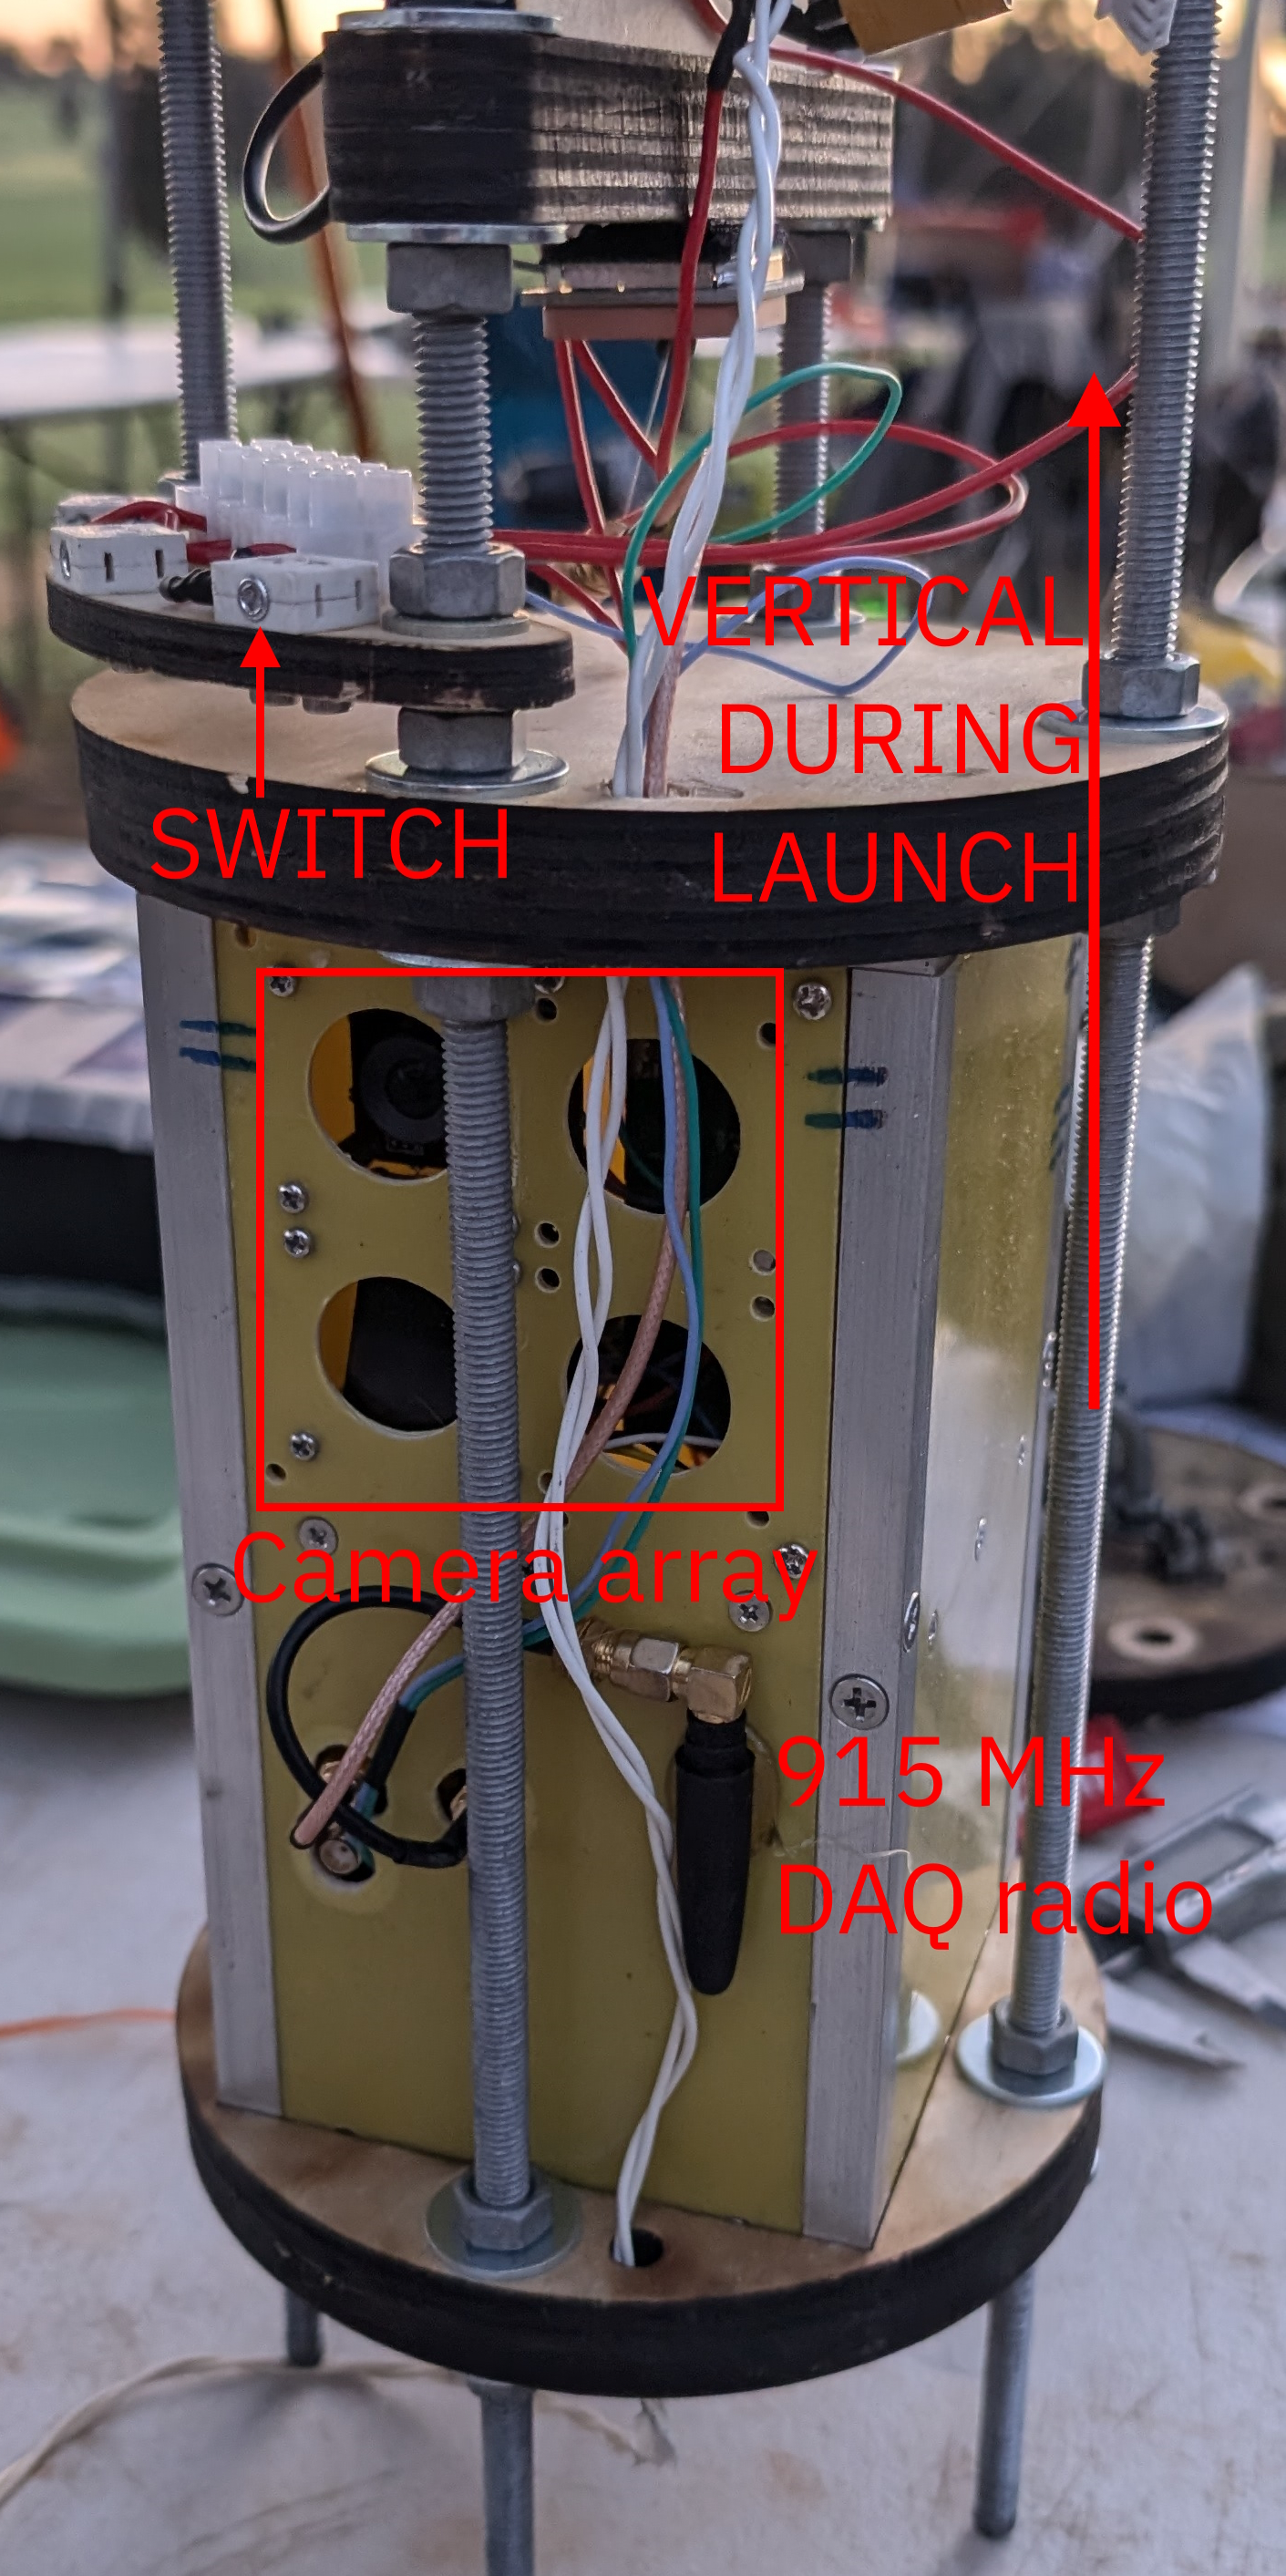
\includegraphics[width=\linewidth]{images/cubesat-payload-bay.jpg}
    \caption{CubeSat mounting hardware before mounting in \textit{UNO}.}
  \end{subfigure}
  \begin{subfigure}{0.495\textwidth}
    \centering
    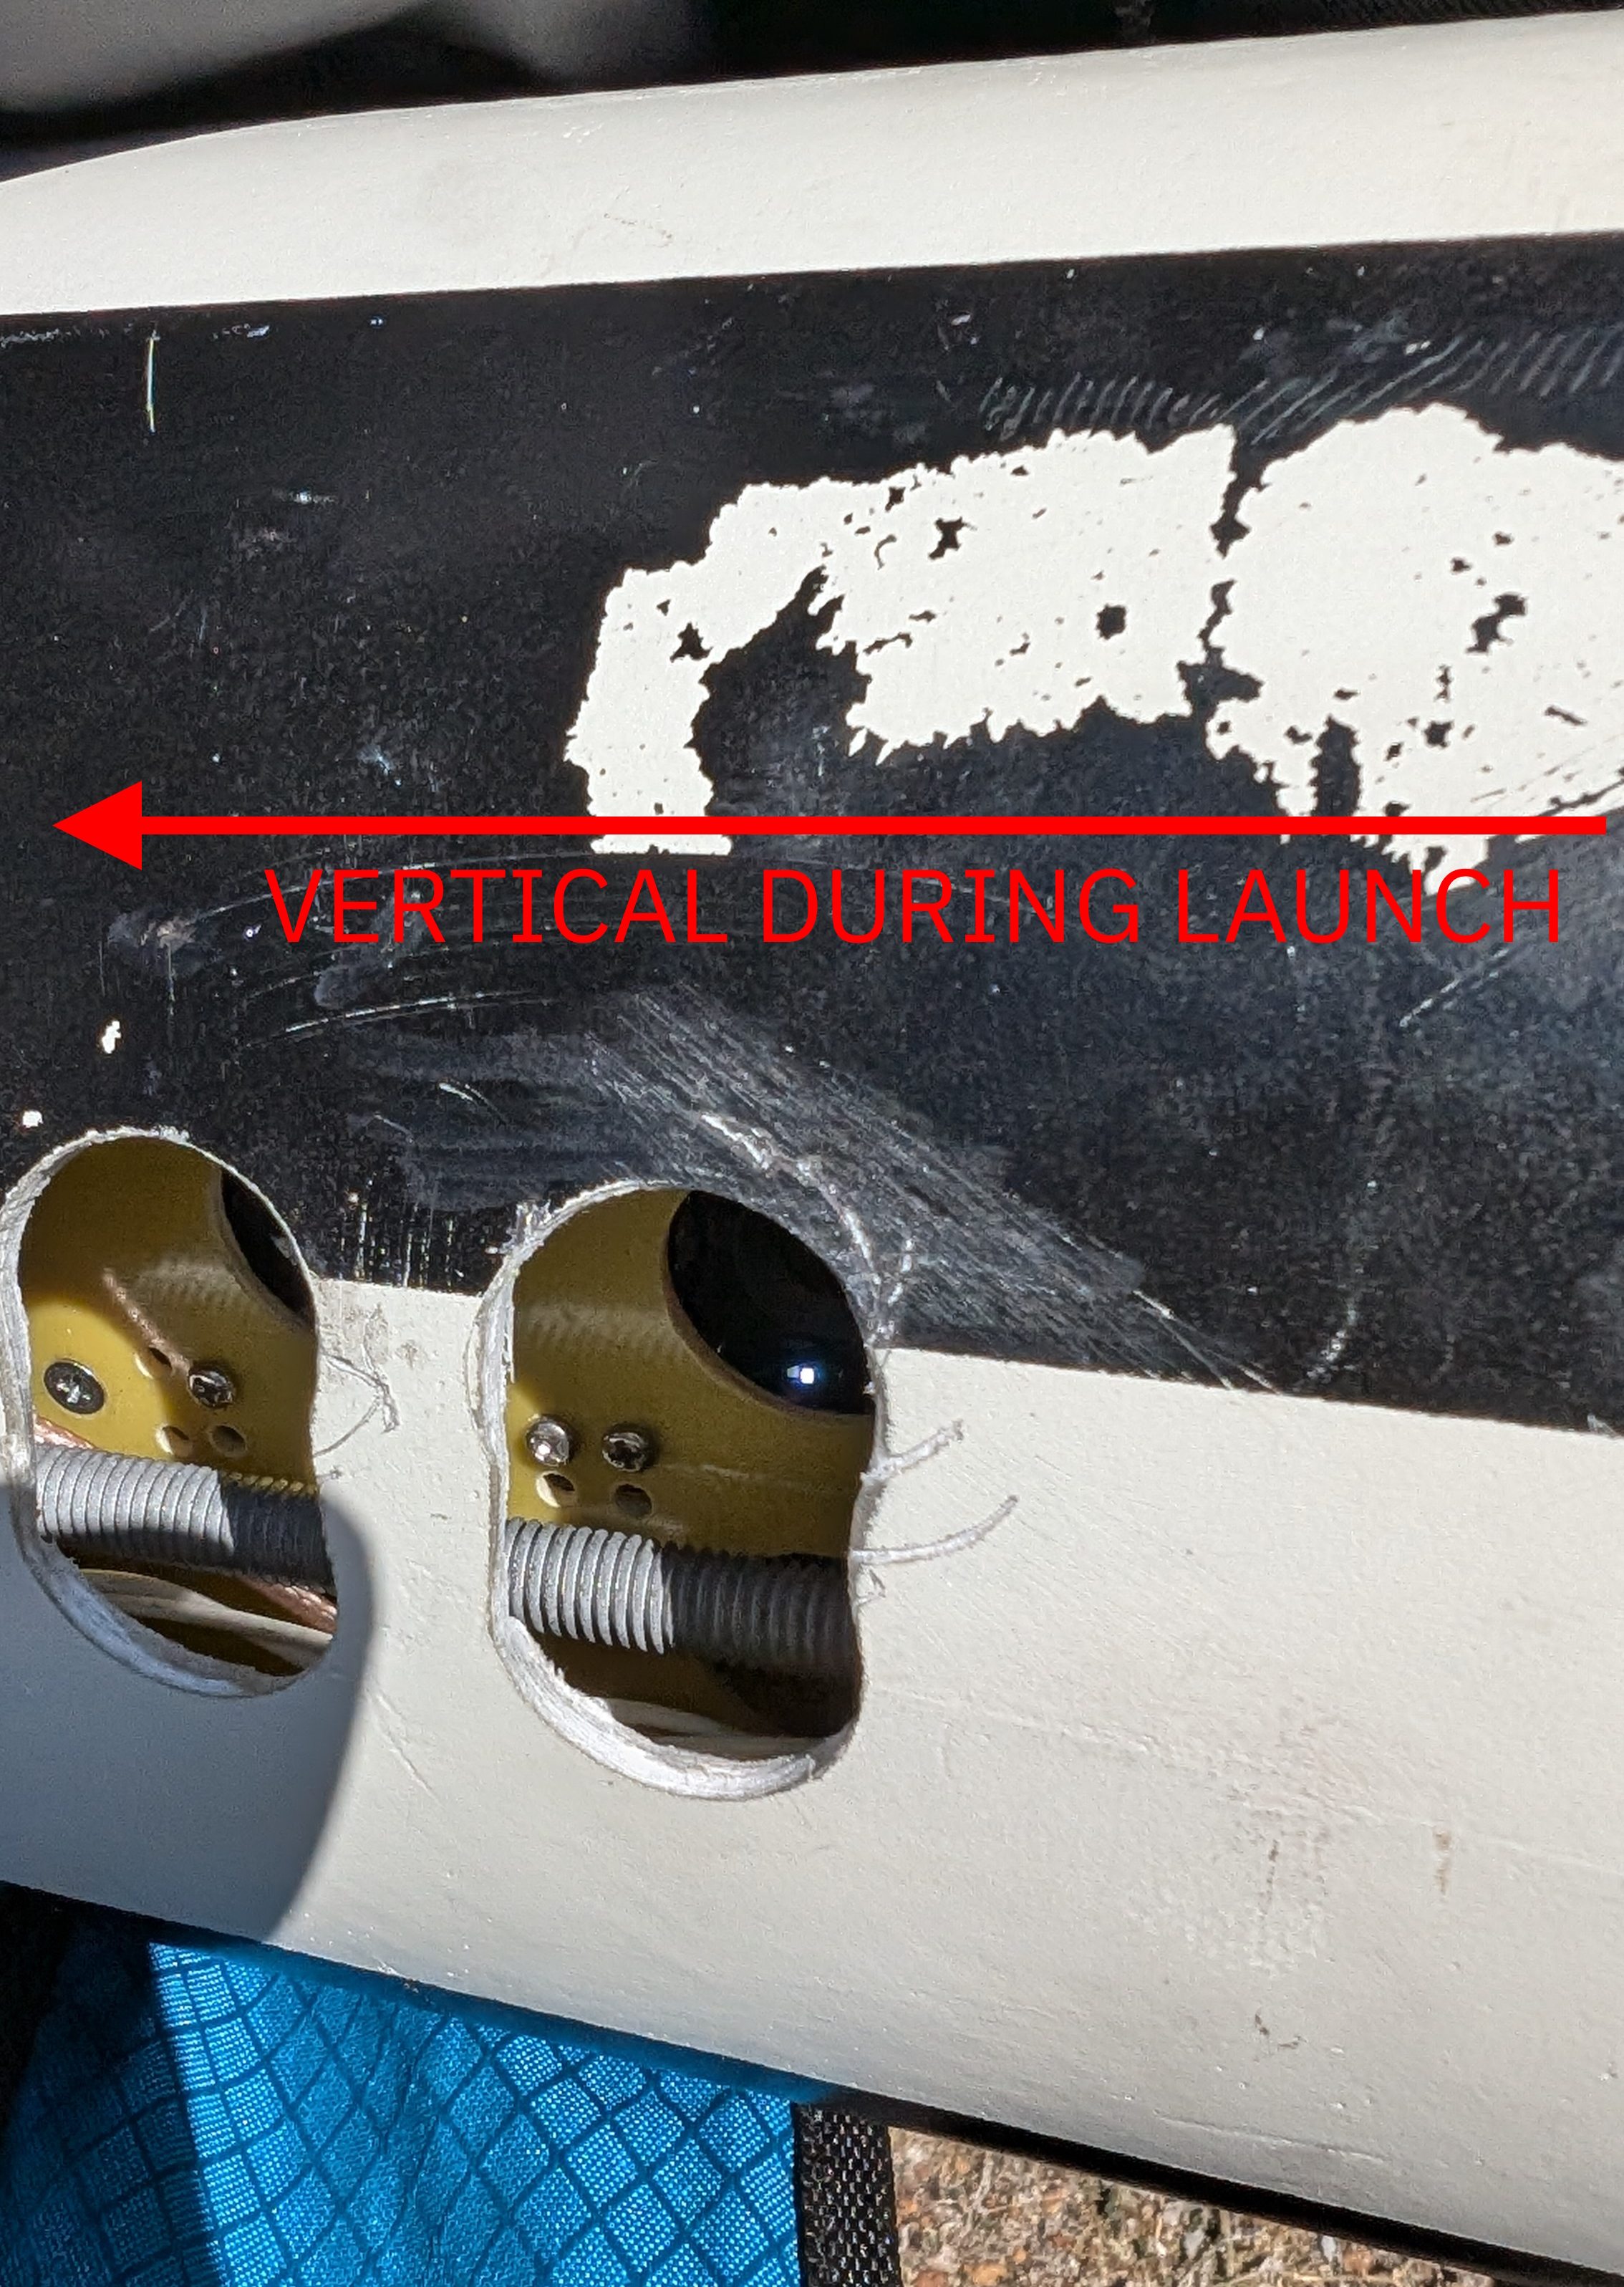
\includegraphics[width=\linewidth]{images/camera-holes.jpg}
    \caption{Camera holes in the side of the rocket body.}
  \end{subfigure}
  \caption{CubeSat in \textit{UNO} before launch.}
  \label{fig:hpr-mounting}
\end{figure}

After mounting the DAQ payload and setting up recovery electronics and parachutes, the K1100T motor was mounted in the motor tube. The rocket was then transported to the launch pad where it was mounted vertically on a launch rail and a motor igniter was attached.

The rocket was launched remotely, and the DAQ continued to save accelerometer data during the flight. A video was taken during flight to label the response to certain flight events.

Once the rocket landed, it was safed by switching off power to the recovery electronics and the DAQ. The recovered rocket was transported back for disassembly and retrieval of the CubeSat.

\subsection{HPR Data Analysis}

After the rocket landed, the accelerometer data files were extracted from the Raspberry Pi's SD card and transferred to a computer. A Python notebook was created to process the data as follows:

\begin{itemize}
  \item Unpack the binary flat file into a CSV.
  \item Plot the CSV.
  \item Visually identify the start of the flight which is characterised by a sustained increase acceleration for a few seconds.
  \item Using video of the flight, identify the end of the flight and all key phases (including boost, coast and pyrotechnic events).
  \item Separate the CSV into smaller CSVs which contain the boost and coast phases and pyroshock events.
  \item For the boost and coast phases, which represent quasi-static acceleration and random vibration respectively, use Welch's method to obtain an estimation of the power spectral density.
  \item For the pyroshock events, originally Welch's method would be used, however it was found that plotting the time-domain shock response was more valuable for this analysis due to frequency limitations of the both accelerometers in the DAQ and shaker table.
\end{itemize}

This process is summarised in figure \ref{fig:hpr-data-processing}.

\begin{figure}[H]
  \centering
  \includesvg[width=0.85\linewidth]{images/hpr-workflow.svg}
  \caption{Data processing workflow for HPR accelerometer data.}
  \label{fig:hpr-data-processing}
\end{figure}

\subsection{Shaker Table Experiment Setup}

\section{Shaker Table}
\label{sec:shaker-table-method}

The shaker table tests were performed at AVI on the \DTMdate{2024-09-25} using a Brüel \& Kjær LDS V8800 electrodynamic shaker table. The CubeSat was fixed to the shaker table using three bolts which went through the bottom plate.

A Brüel \& Kjær type 4533-B integrated electronics piezoelectric (IEPE) accelerometer was used as the control and data accelerometer, which were mounted to the shaker table and the payload respectively. This accelerometer has a frequency range of \SI{0.016}{\hertz} to \SI{1250}{\kilo\hertz} and a resonance frequency of \SI{36.7}{\kilo\hertz}, which is well above the range of the tests. The accelerometers were attached to mounting studs which were fixed to the CubeSat using bisphenol-A epoxy.

The table was first mounted in the vertical configuration and the CubeSat was mounted axially as shown in figure \ref{fig:shaker-axis-setup}. Random and shock tests were performed, then the table was rotated manually \SI{90}{\degree} and the CubeSat re-mounted to conduct the same tests in the x-axis. The CubeSat was rotated \SI{90}{\degree} to finally test the y-axis.

\begin{figure}[H]
  \begin{subfigure}{0.32\textwidth}
    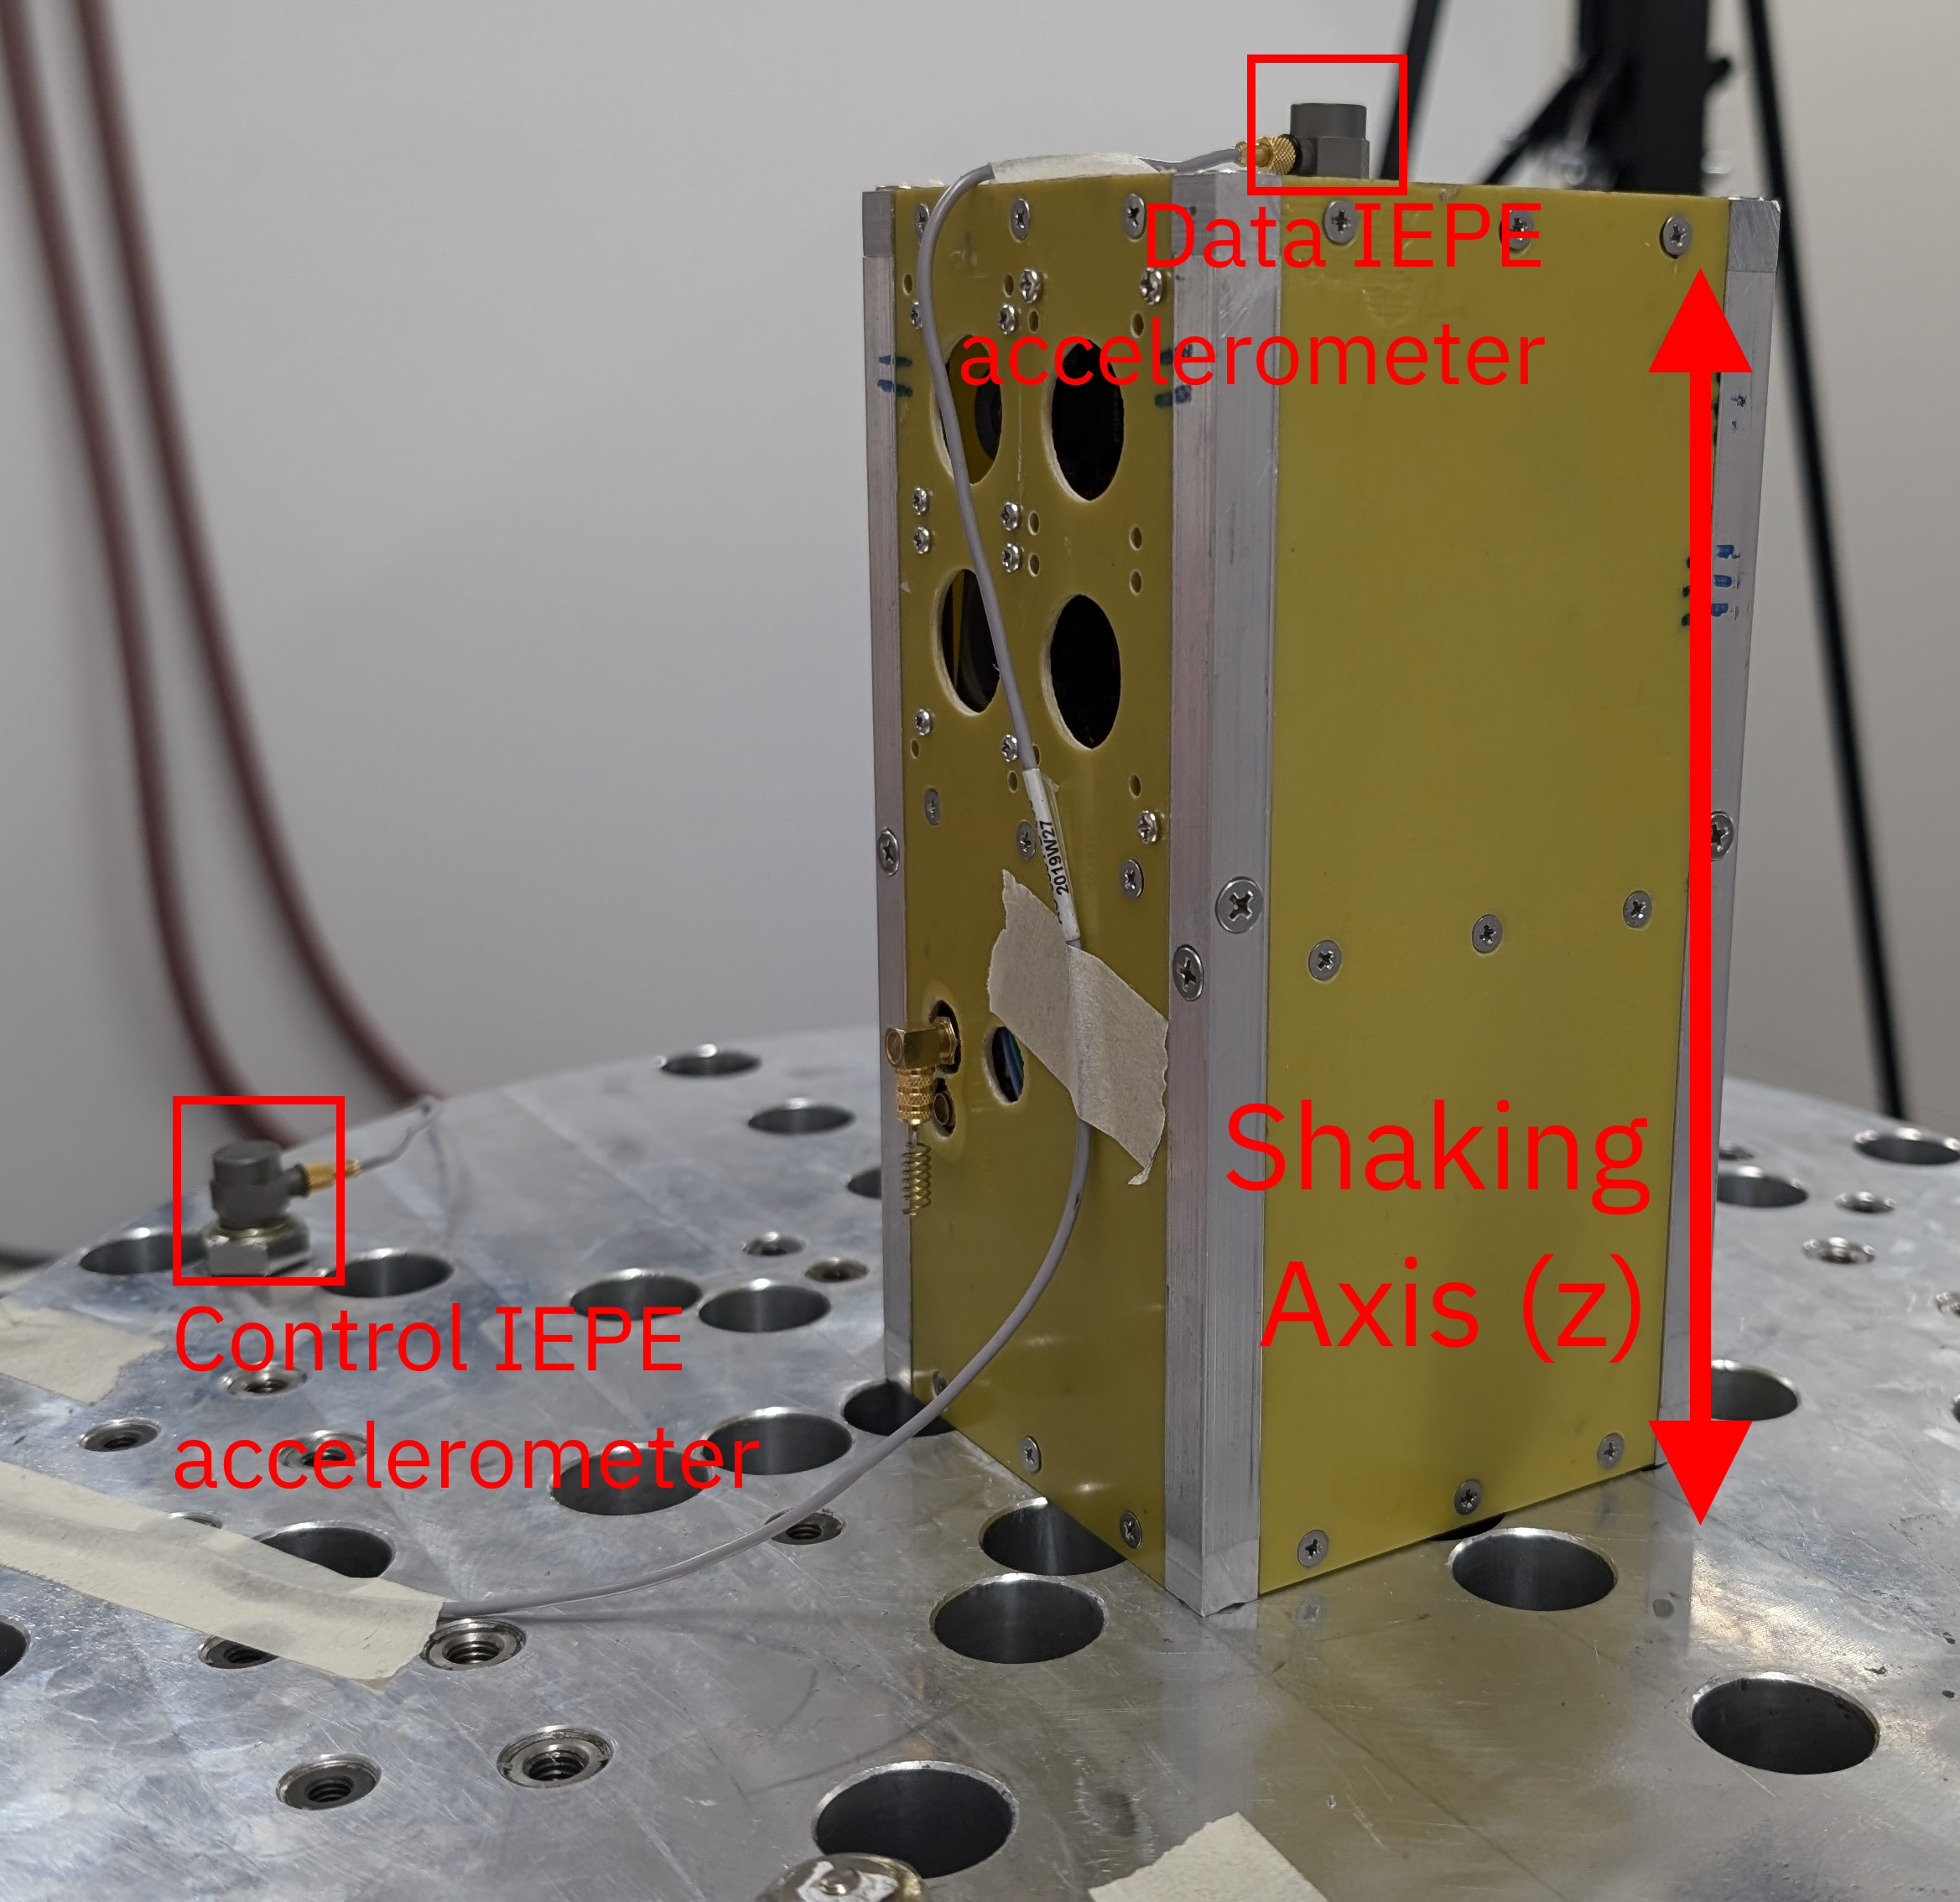
\includegraphics[width=\linewidth]{images/z-axis-setup.jpg}
    \caption{z-axis}
  \end{subfigure}
  \begin{subfigure}{0.32\textwidth}
    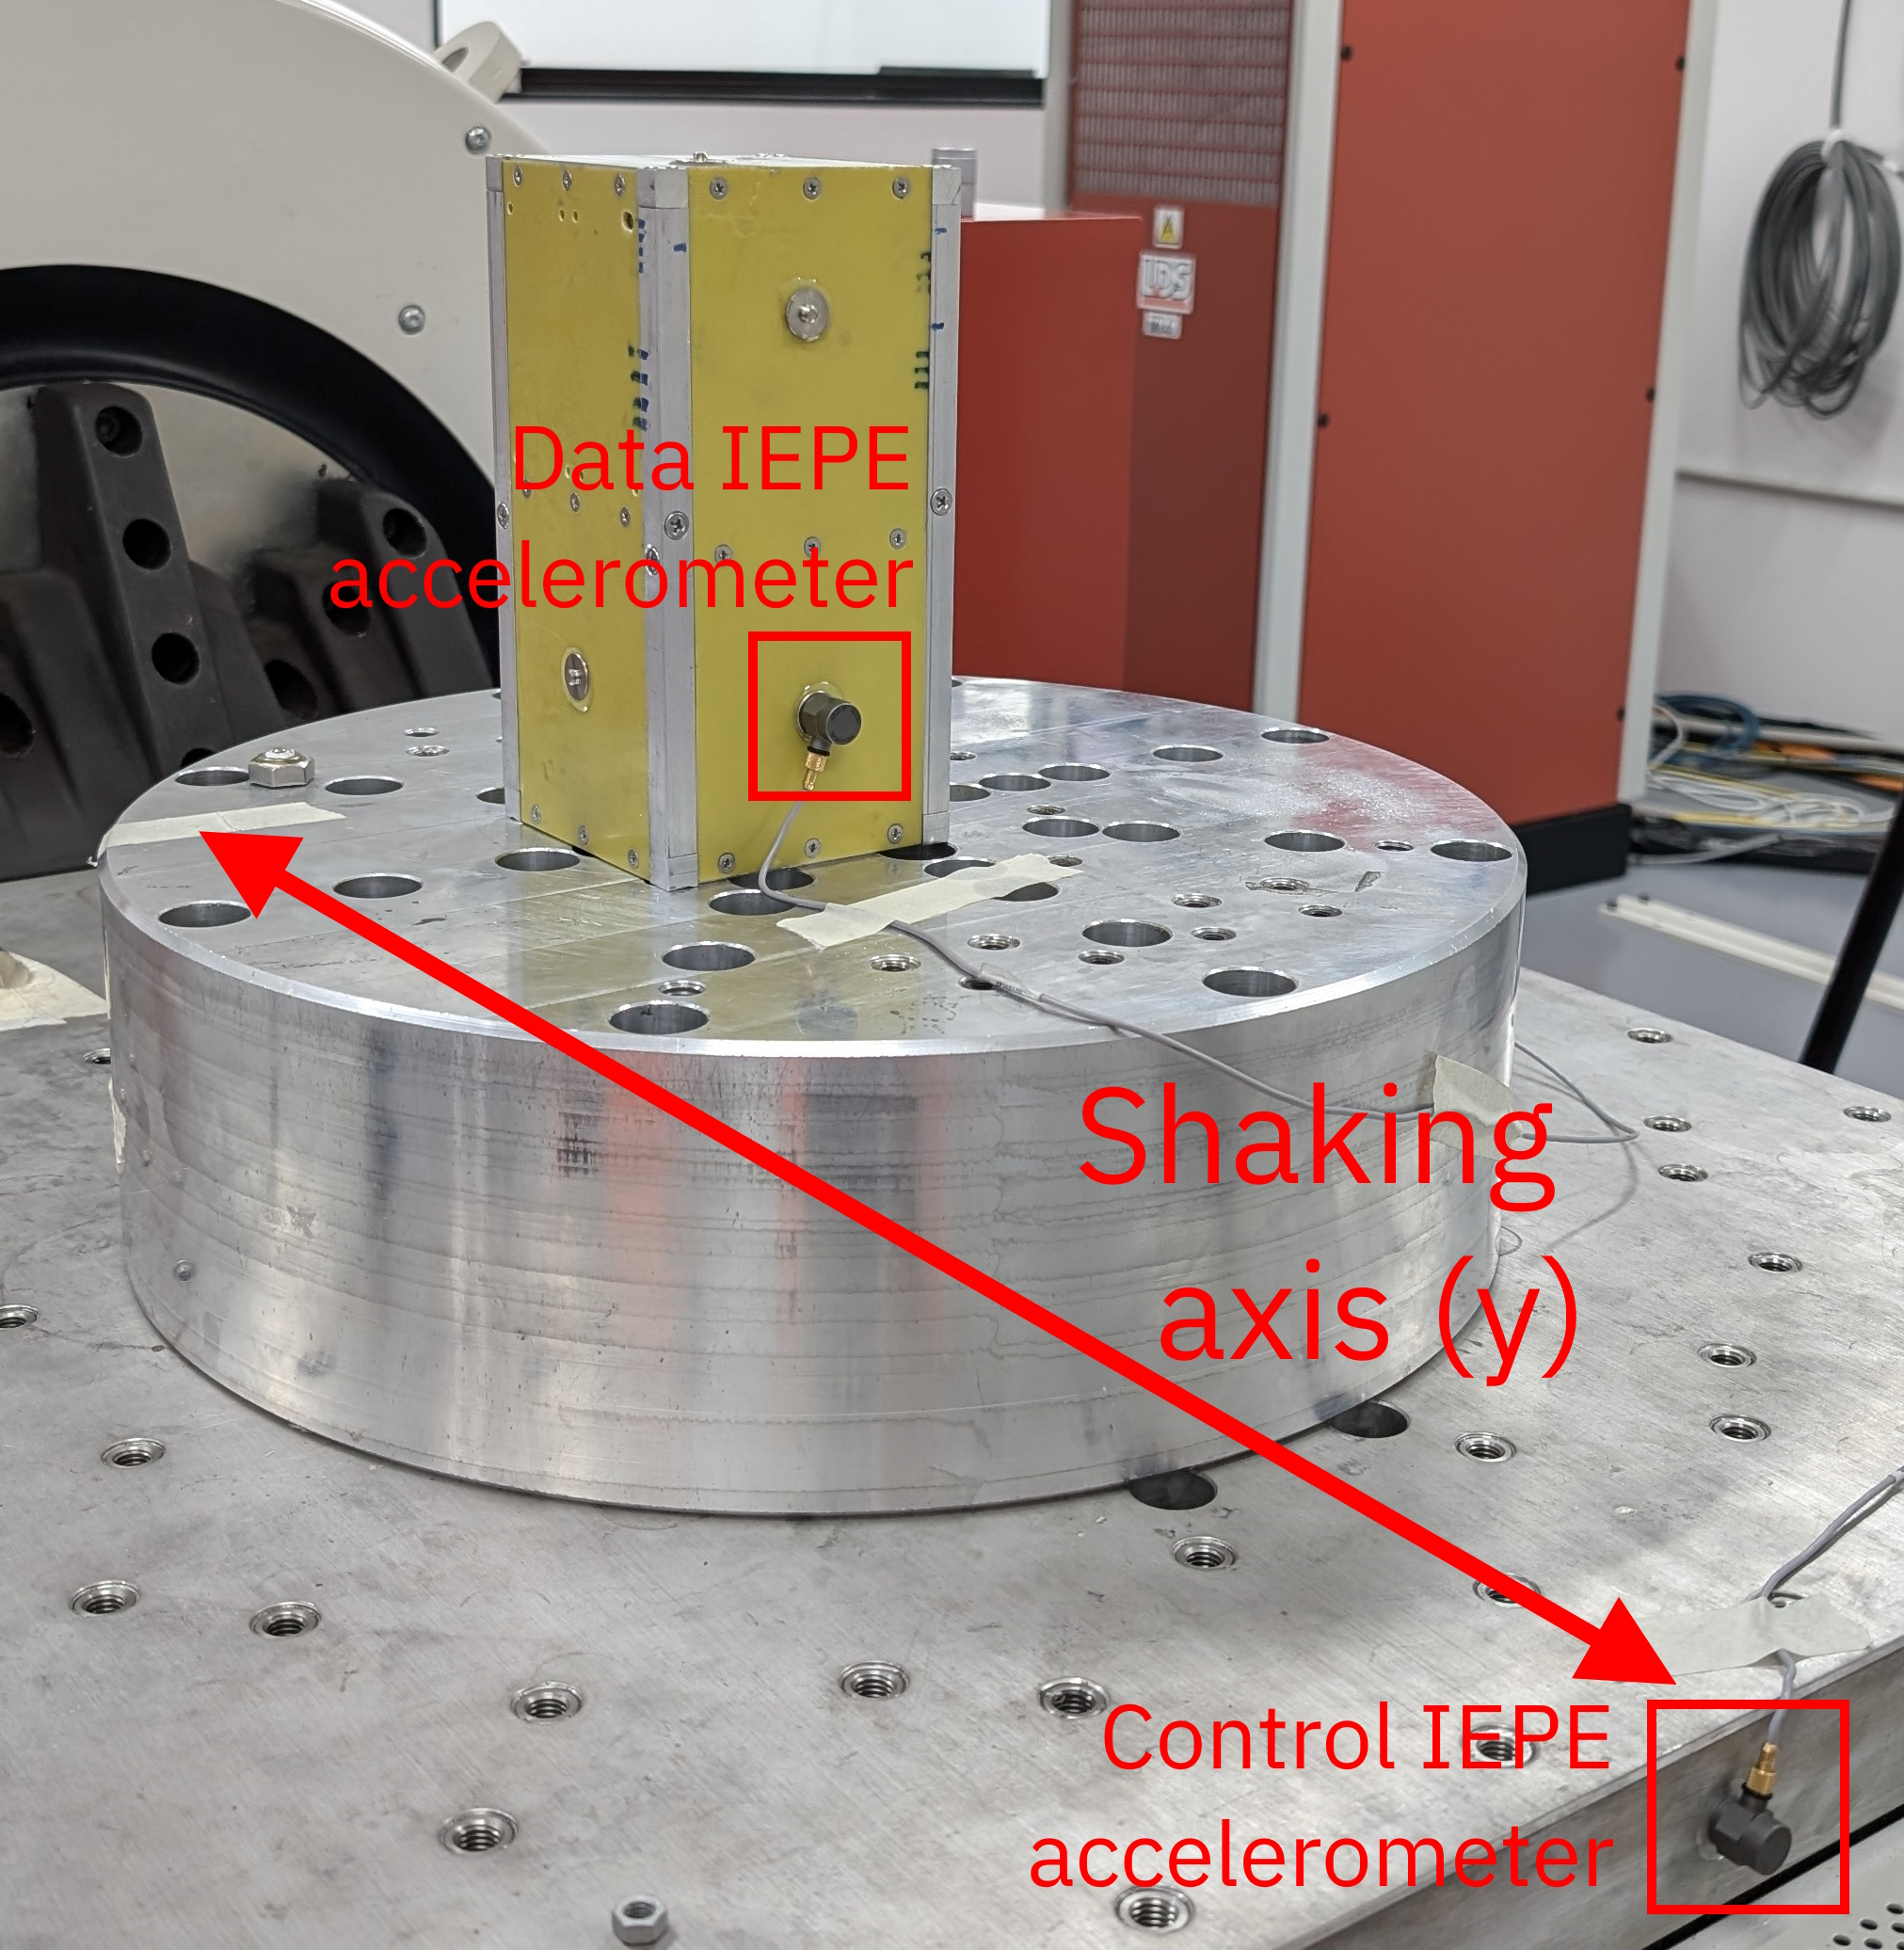
\includegraphics[width=\linewidth]{images/y-axis-setup.jpg}
    \caption{y-axis}
  \end{subfigure}
  \begin{subfigure}{0.32\textwidth}
    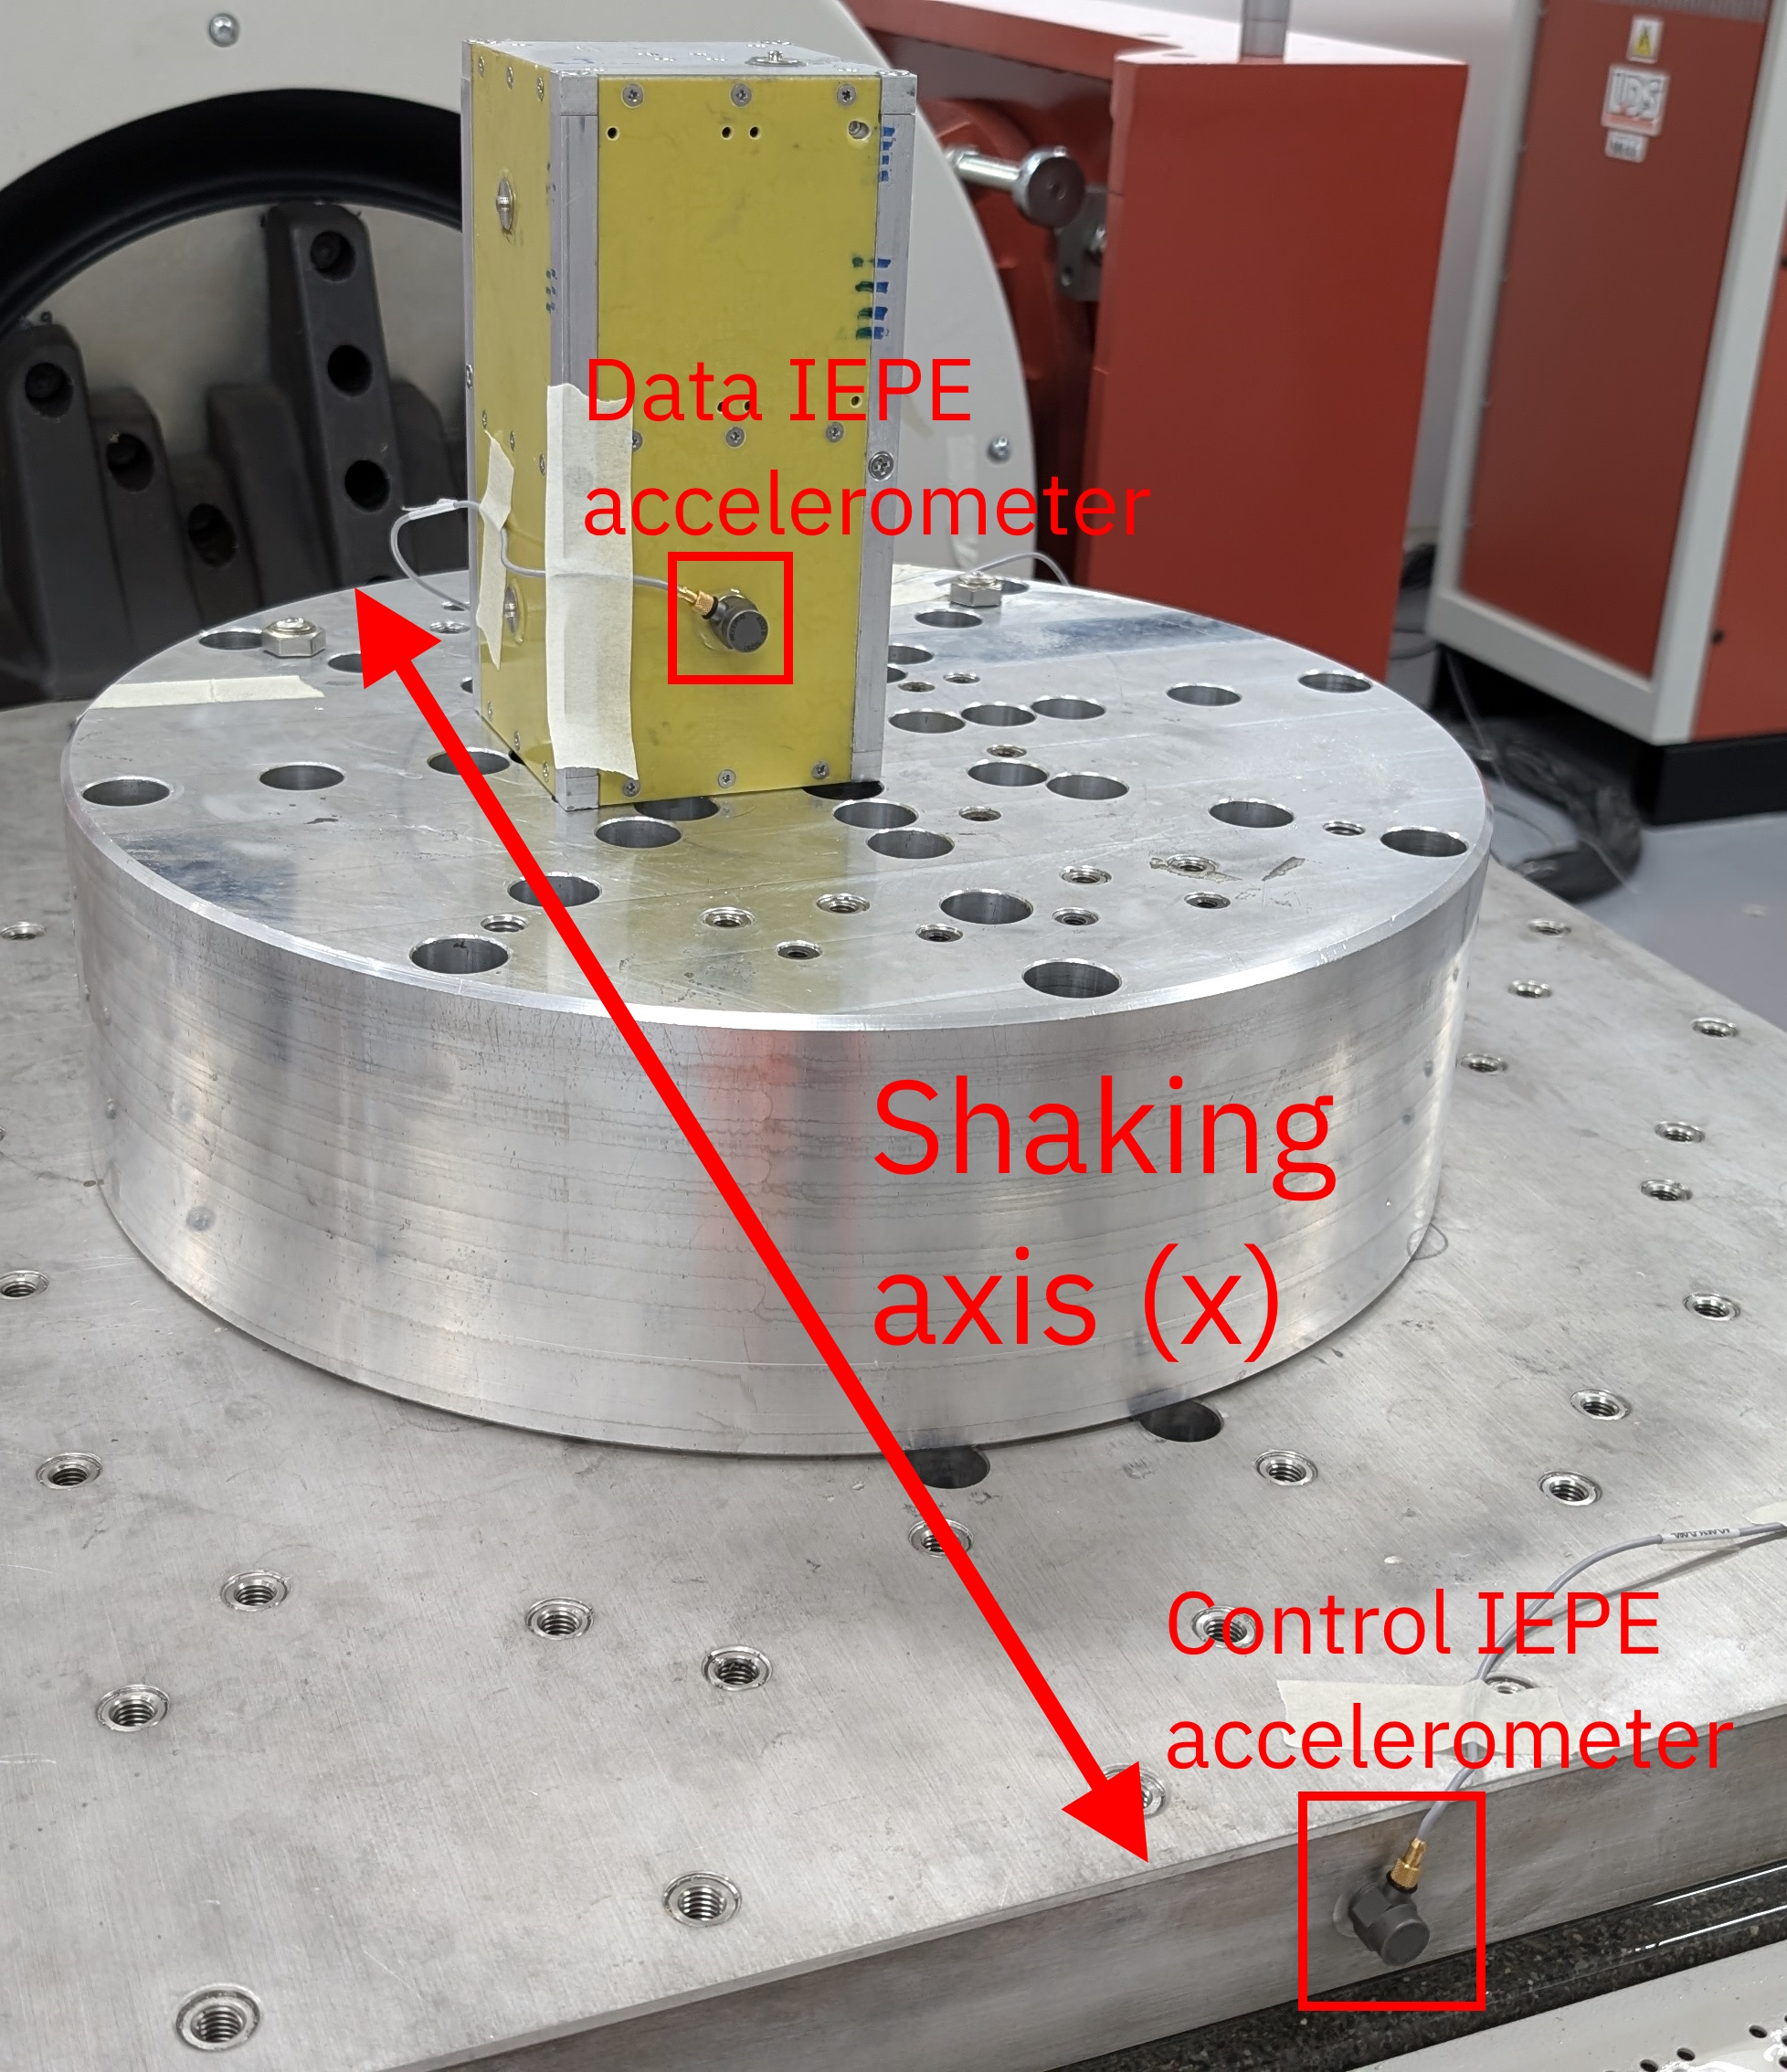
\includegraphics[width=\linewidth]{images/x-axis-setup.jpg}
    \caption{x-axis}
  \end{subfigure}
  \caption{CubeSat setup in on the shaker table.}
  \label{fig:shaker-axis-setup}
\end{figure}

\subsection{Random}

The IIST recommended random vibration profile described in table \ref{tabl:random-vibration-profile-iist} was used.

% \subsection{Sine-Sweep}

% The sine-sweep profile described in table \ref{tabl:sine-sweep-profile-iist} was found to not be realisable on the shaker table since the profile described requires all three axes to be simultaneously driven. To replicate shaker table test where all three axes are simultaneously driven using one axis, the single axis must be driven with 2.5 times the $g_\text{rms}$ \cite{nath2022study}. A second attempt used the single-axis modified test shown in table \ref{tabl:sine-sweep-mod1}


% \begin{table}[H]
%   \centering
%   \begin{tabular}{|c|c|c|c|}
%     \hline
%     \textbf{Frequency}        & \textbf{Level}     & \textbf{Sweep Rate}        & \textbf{Axis} \\\hline
%     \SI{10}{\hertz}           & \SI{13.198}{\gacc} & \SI{4}{\octave\per\minute} & Longitudinal  \\\hline
%     \SI{12}{\hertz}           & \SI{19.006}{\gacc} & \SI{4}{\octave\per\minute} & Longitudinal  \\\hline
%     \SI{14}{\hertz}           & \SI{25.869}{\gacc} & \SI{4}{\octave\per\minute} & Longitudinal  \\\hline
%     \SIrange{16}{100}{\hertz} & \SI{32.79}{\gacc}  & \SI{4}{\octave\per\minute} & Longitudinal  \\\hline
%   \end{tabular}
%   \caption{First modification of IIST 3-axis sine-sweep profile to a single axis.}
%   \label{tabl:sine-sweep-mod1}
% \end{table}

% Due to the low frequencies with high acceleration, this profile was not realisable by the shaker table and resulted in an alarm being raised by the machine. Through trial and error it was found the profile described in table \ref{tabl:sine-sweep-mod2} was realisable. This profile discarded the low frequencies below \SI{30}{\hertz}.

% \begin{table}[H]
%   \centering
%   \begin{tabular}{|c|c|c|c|}
%     \hline
%     \textbf{Frequency}        & \textbf{Level}    & \textbf{Sweep Rate}        & \textbf{Axis} \\\hline
%     \SIrange{30}{100}{\hertz} & \SI{20}{\gacc} & \SI{4}{\octave\per\minute} & Longitudinal  \\\hline
%   \end{tabular}
%   \caption{Realisable modification of IIST 3-axis sine-sweep profile.}
%   \label{tabl:sine-sweep-mod2}
% \end{table}

\subsection{Quasi-static Acceleration Test}

A QAT was not specified by IIST, therefore one was created which has a profile of \SI{18.9}{\gacc} from \SIrange{30}{35}{\hertz}. However, this test was not realisable with the type of shaker table after testing. Since IIST did not specify this test, it was excluded from testing. For later analysis, the boost phase would be compared to random vibration.

\subsection{Shock}

Due to limitations of the shaker table, the shock time had to be reduced from \SI{10}{\milli\second} to \SI{8}{\milli\second}, which produced a shock which would over-qualify the CubeSat compared to the IIST recommended profile. The profile is shown in figure \ref{fig:shock-table-profile}

\begin{figure}[H]
  \centering
  \includesvg[width=\linewidth]{images/shock_table_profiel.svg}
  \caption{Realised shock profile.}
  \label{fig:shock-table-profile}
\end{figure}

\section{Evaluation of HPR as a CubeSat Qualification Platform}

Each part of flight is compared to one type of shaker table test as shown in table \ref{tabl:compare-tests}:

\begin{table}[H]
  \centering
  \begin{tabular}{|c|c|c|}
    \hline
    \textbf{HPR flight}            & \textbf{Shaker table} & \textbf{Representation} \\\hline
    Boost/launch                   & Random vibration      & PSD                     \\\hline
    Coast                          & Random vibration      & PSD                     \\\hline
    Pyroshock/parachute deployment & Shock                 & SRS, Time domain        \\\hline
  \end{tabular}
  \caption{Comparisons between the two tests and their representation.}
  \label{tabl:compare-tests}
\end{table}

Since the shaker table profiles are at or above the IIST recommended qualification level, for this research it will be assumed this was adequate to qualify for launch conditions.

HPR will be a successful qualification platform if:
\begin{itemize}
  \item For PSD measurements the HPR PSD trace is equal to or greater than the PSD trace from the corresponding shaker table test.
  \item For shock, the HPR pyroshock events should produce a shock response which has a half-sine profile time which is less than the shaker table response, and a peak acceleration which is greater than the shaker table response.
\end{itemize}

\chapter{DAQ Evaluation and Discussion}

\section{Drone Tests}
\subsection{First Drone Test}

The first drone test was performed on the \DTMdate{2024-7-8} at the UWA Shenton Park Field Station. At this stage in development, the first iteration of the design was partially completed. This was mounted to a 3d-printed mockup of the final CubeSat chassis, then tied to the drone, as shown in figure \ref{fig:drone-cube-1}. In this configuration, the camera payload is in the top half of the CubeSats and the DAQ in the bottom half. The camera payload is mounted so that the camera is pointing towards the ground. A DJI M600 drone was used to raise the CubeSat to \SI{120}{\metre}.

Since at this point in the design process it was evaluated that the DAQ needed a second new design, most of the systems were not tested, and the focus was on testing the camera payload. The DAQ's EPS was tested in this flight since it was needed for the camera to capture an image.

As a test of the DAQ's EPS, this test was a complete success since it was able to deliver power to the camera payload throughout the duration of the flight, therefore the EPS was used in the final DAQ design. While not relevant to the evaluation of this system, it should be noted that the camera payload did not capture any images due to a faulty connection between the Raspberry Pi 3 compute module and the camera module on the camera payload.

\begin{figure}[H]
  \centering
  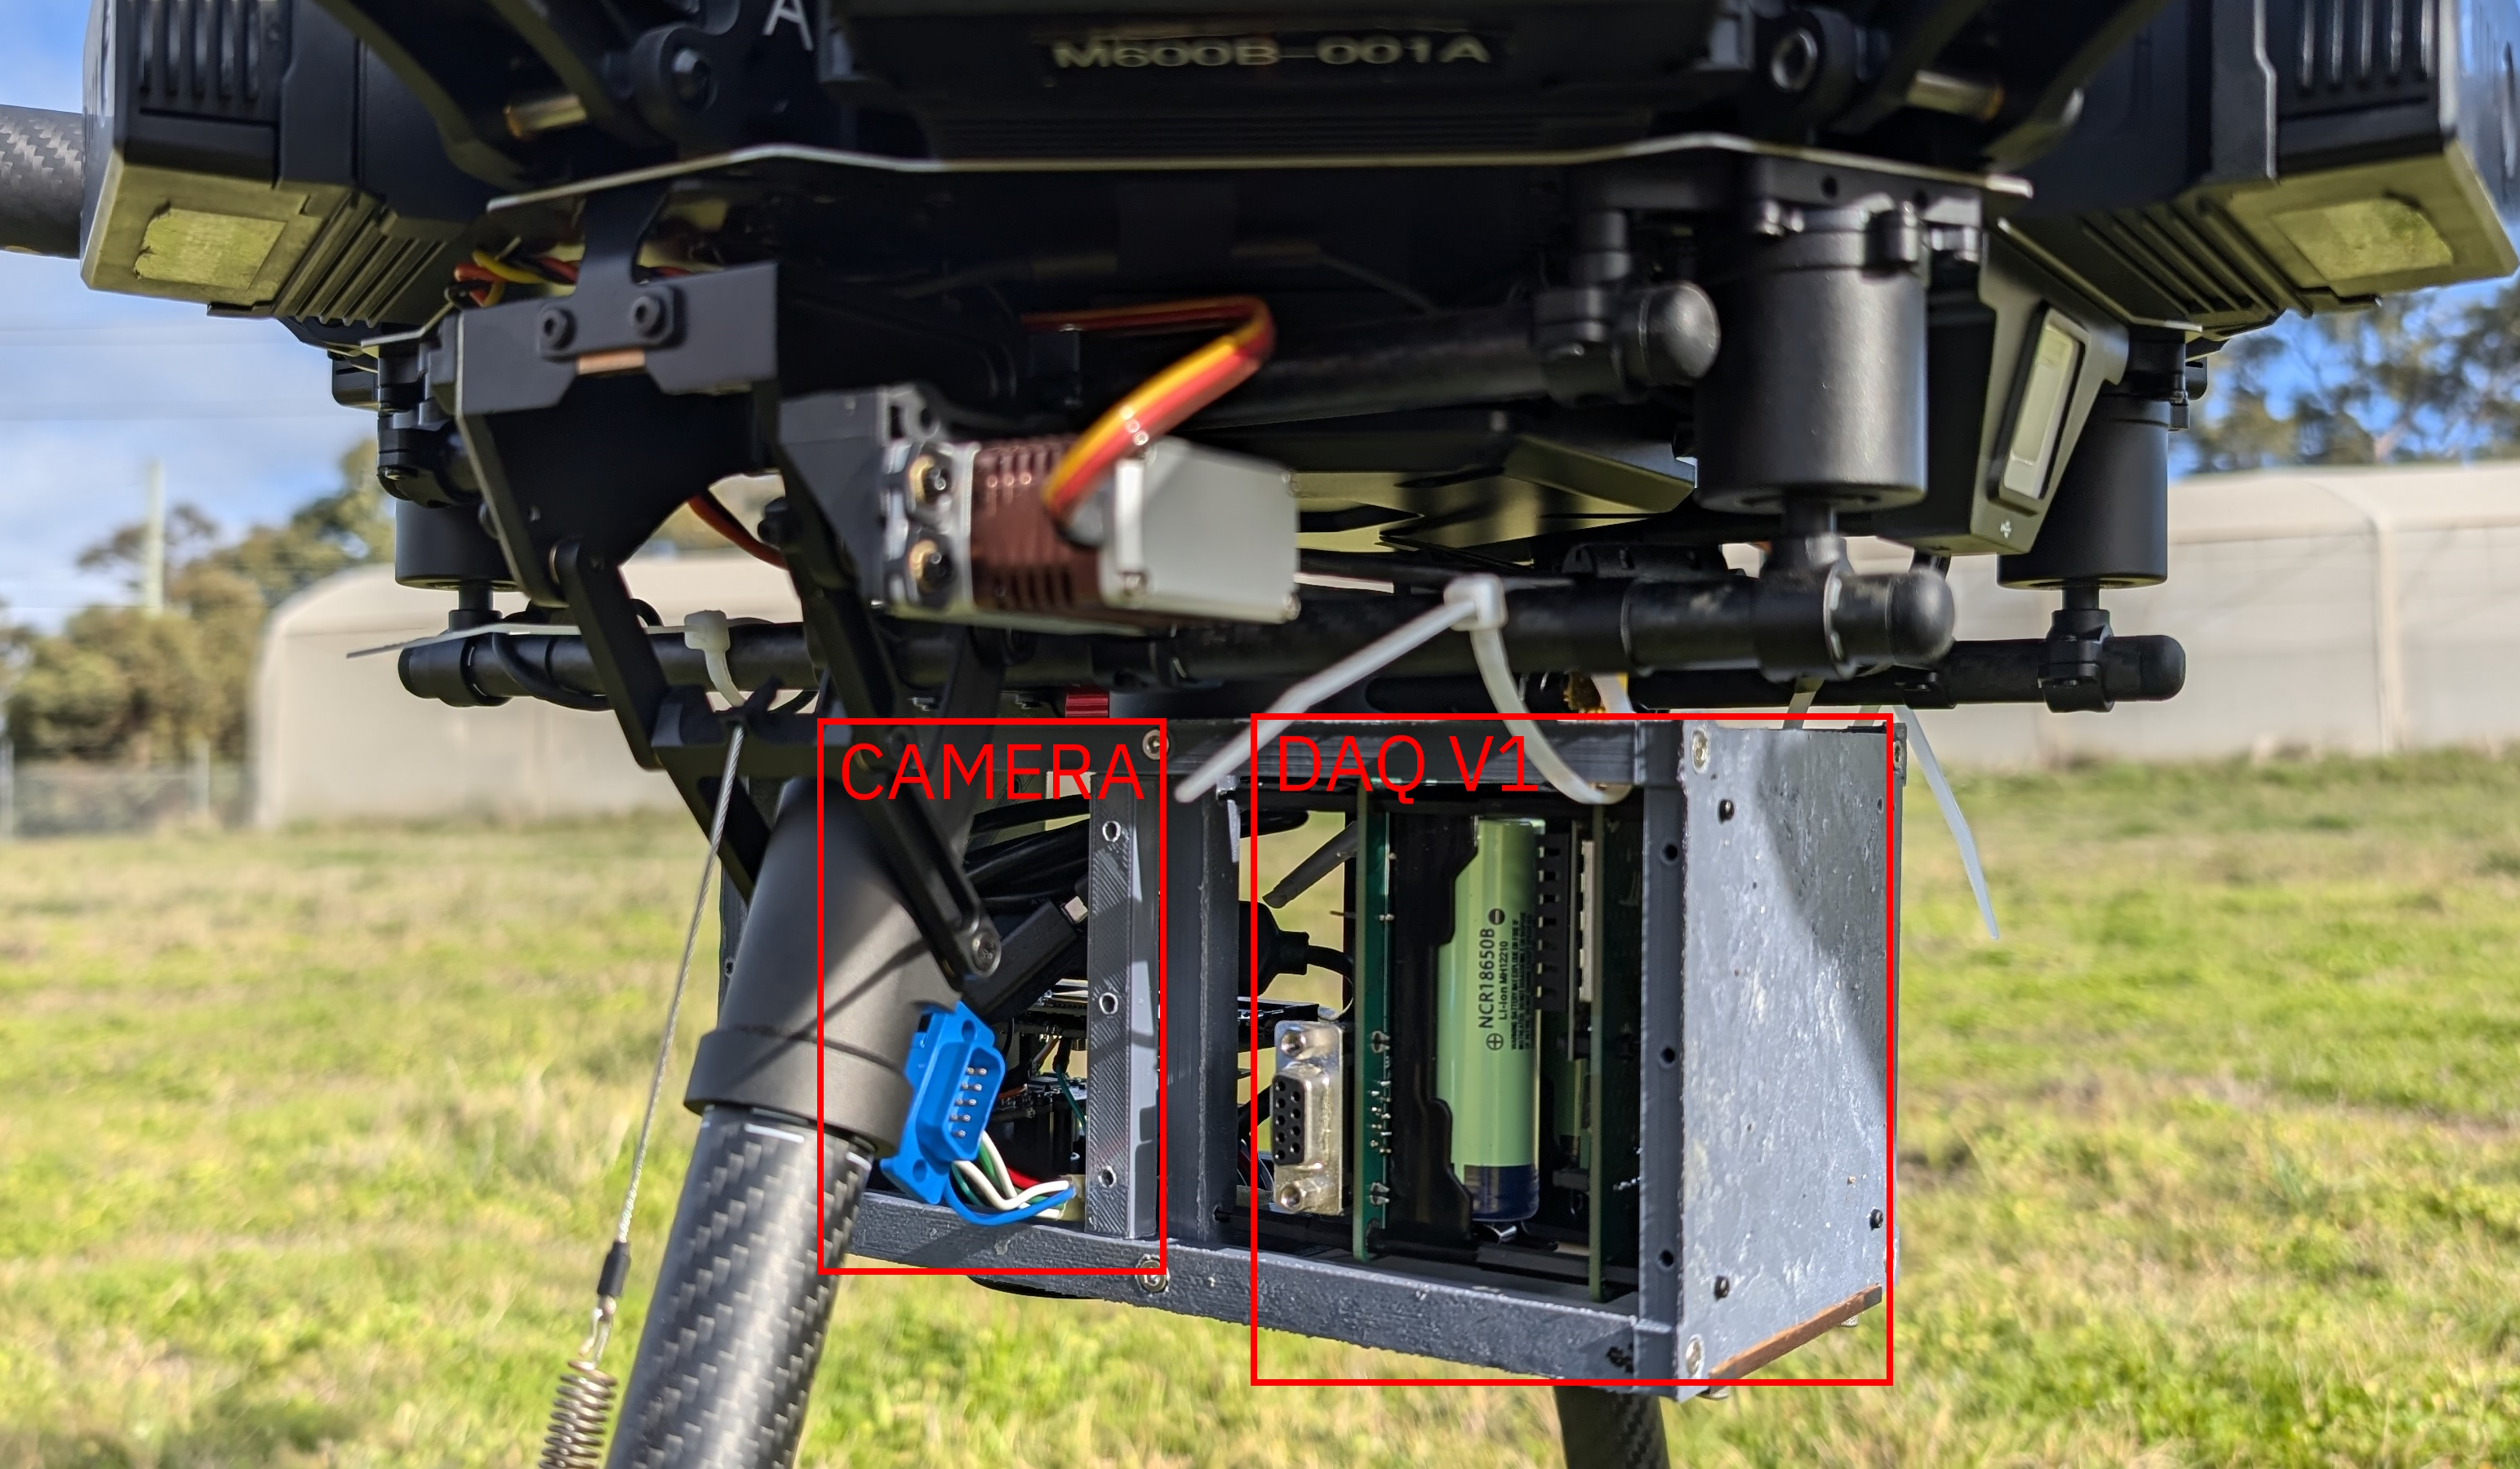
\includegraphics[width=0.9\linewidth]{images/1st_flight_drone_cube.jpg}
  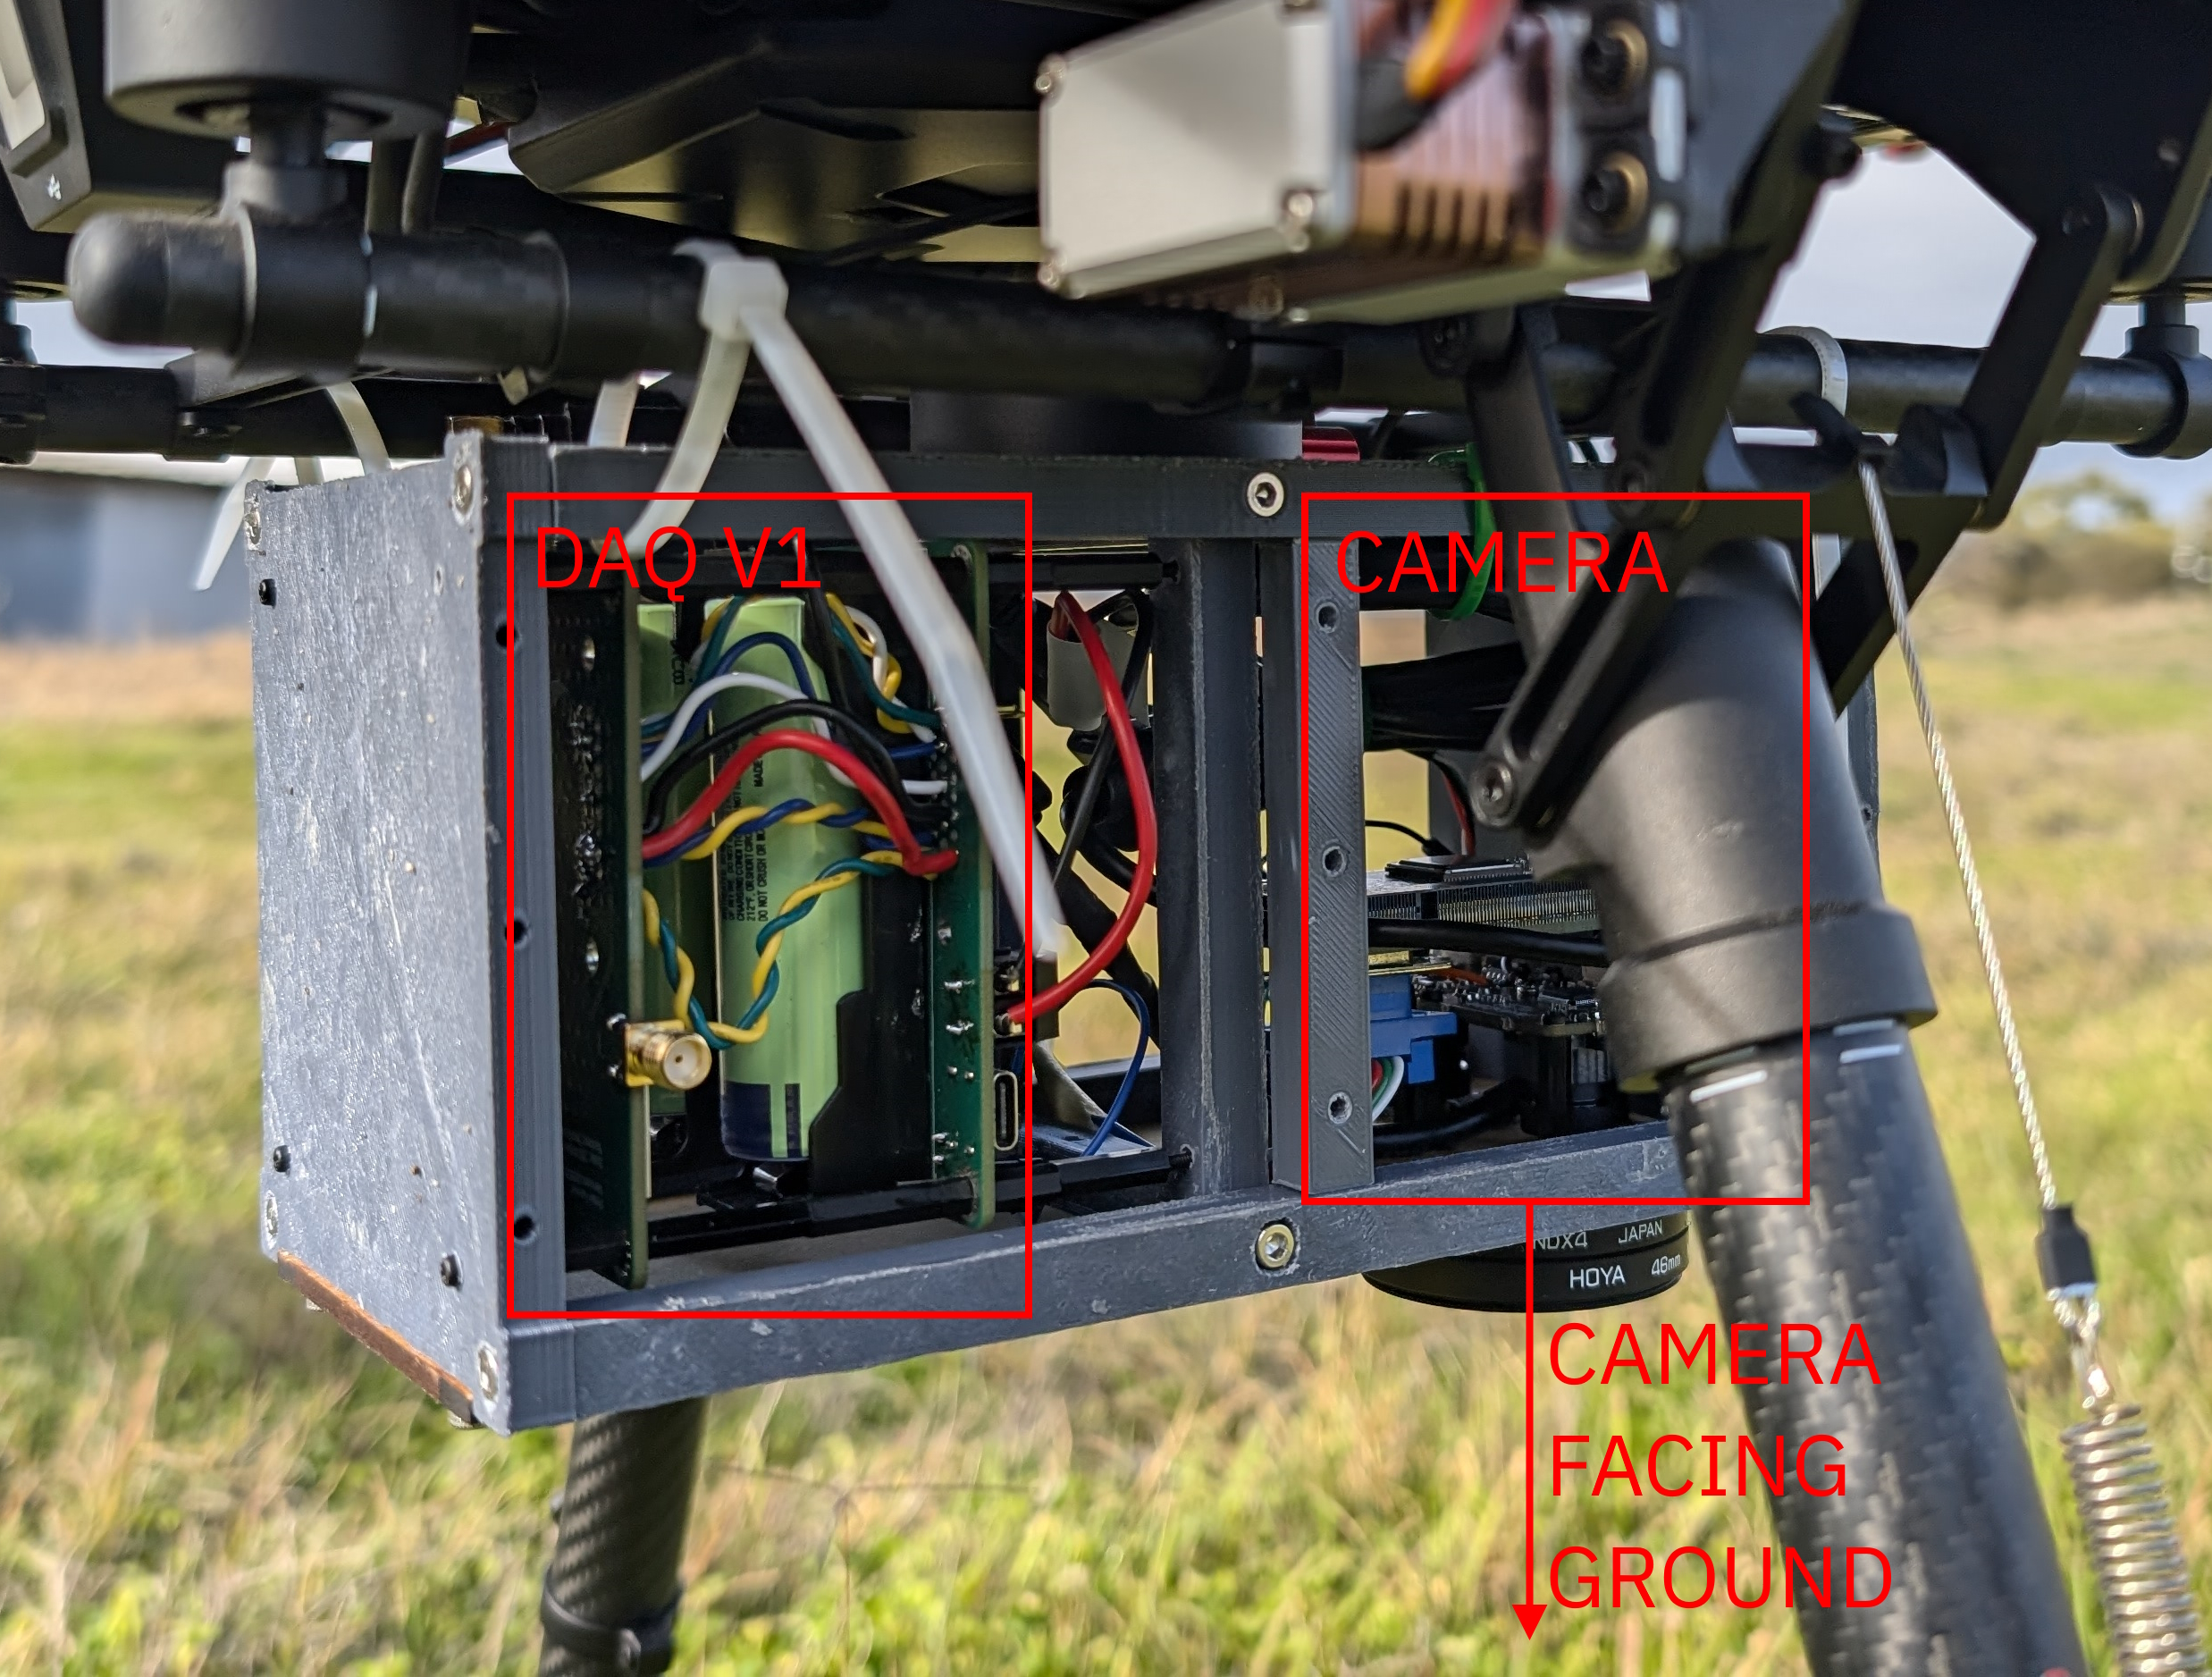
\includegraphics[width=0.9\linewidth]{images/1st_flight_drone_cube_2.jpg}
  \caption{DJI M600 drone with CubeSat mounted sideways before flight.}
  \label{fig:drone-cube-1}
\end{figure}

\subsection{Second Drone Test}
The second drone test was performed on the \DTMdate{2024-9-2} at the UWA Shenton Park Field Station. This drone test uses the final design of the DAQ, final metal CubeSat chassis and a modified camera payload. The CubeSat was mounted to the bottom of the DJI M600 drone in an identical orientation to the first drone test. The drone raised the CubeSat to \SI{120}{\metre}.

As of this test, part of the  final design was programmed, including the radio and CubeSat communications. A message is periodically sent to indicate that the OBDH system is alive.

Due to an issue on the camera payload, no picture data was saved to the OBDH's storage, nor was any picture data was received over the radio link. The periodic messages were received on the ground throughout the flight with the correct system uptime, indicating that the OBDH and radio downlink was stable throughout the flight.

\begin{figure}[H]
  \centering
  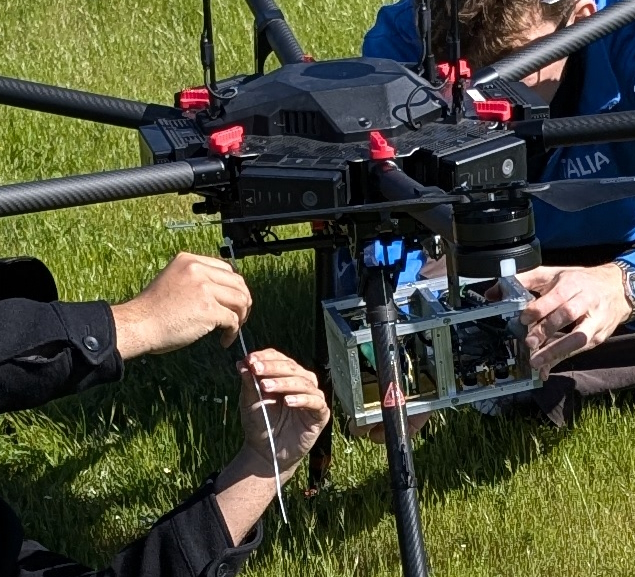
\includegraphics[width=\linewidth]{images/2nd_drone_test_setup.jpg}
  \caption{Mounting the CubeSat to the DJI M600 drone for the second drone test.}
  \label{fig:mounting-cubesat-drone-2}
\end{figure}

\subsection{Third Drone Test}

The third drone test was performed on the \DTMdate{2024-9-12} at the UWA Shenton Park Field Station. All electronic and mechanical hardware was identical between the second test, the only changes were software. This test features the blocking image transmission method after validation of the method in ground testing. The camera payload had other software improvements, including a process watchdog to ensure the system restarts if it encounters an error, and better logging.

This test was a complete success, as two good pictures were captured from the camera system and downloaded to the ground station over the radio link.

A first image was captured at \SI{120}{\metre} above some sheds on the property during the first flight as shown in figure \ref{fig:sheds-received}. The drone was landed in between image captures since the download process uses significant time, and keeping the drone in the air would use battery energy that would be useful for a second image.

\begin{figure}[H]
  \centering
  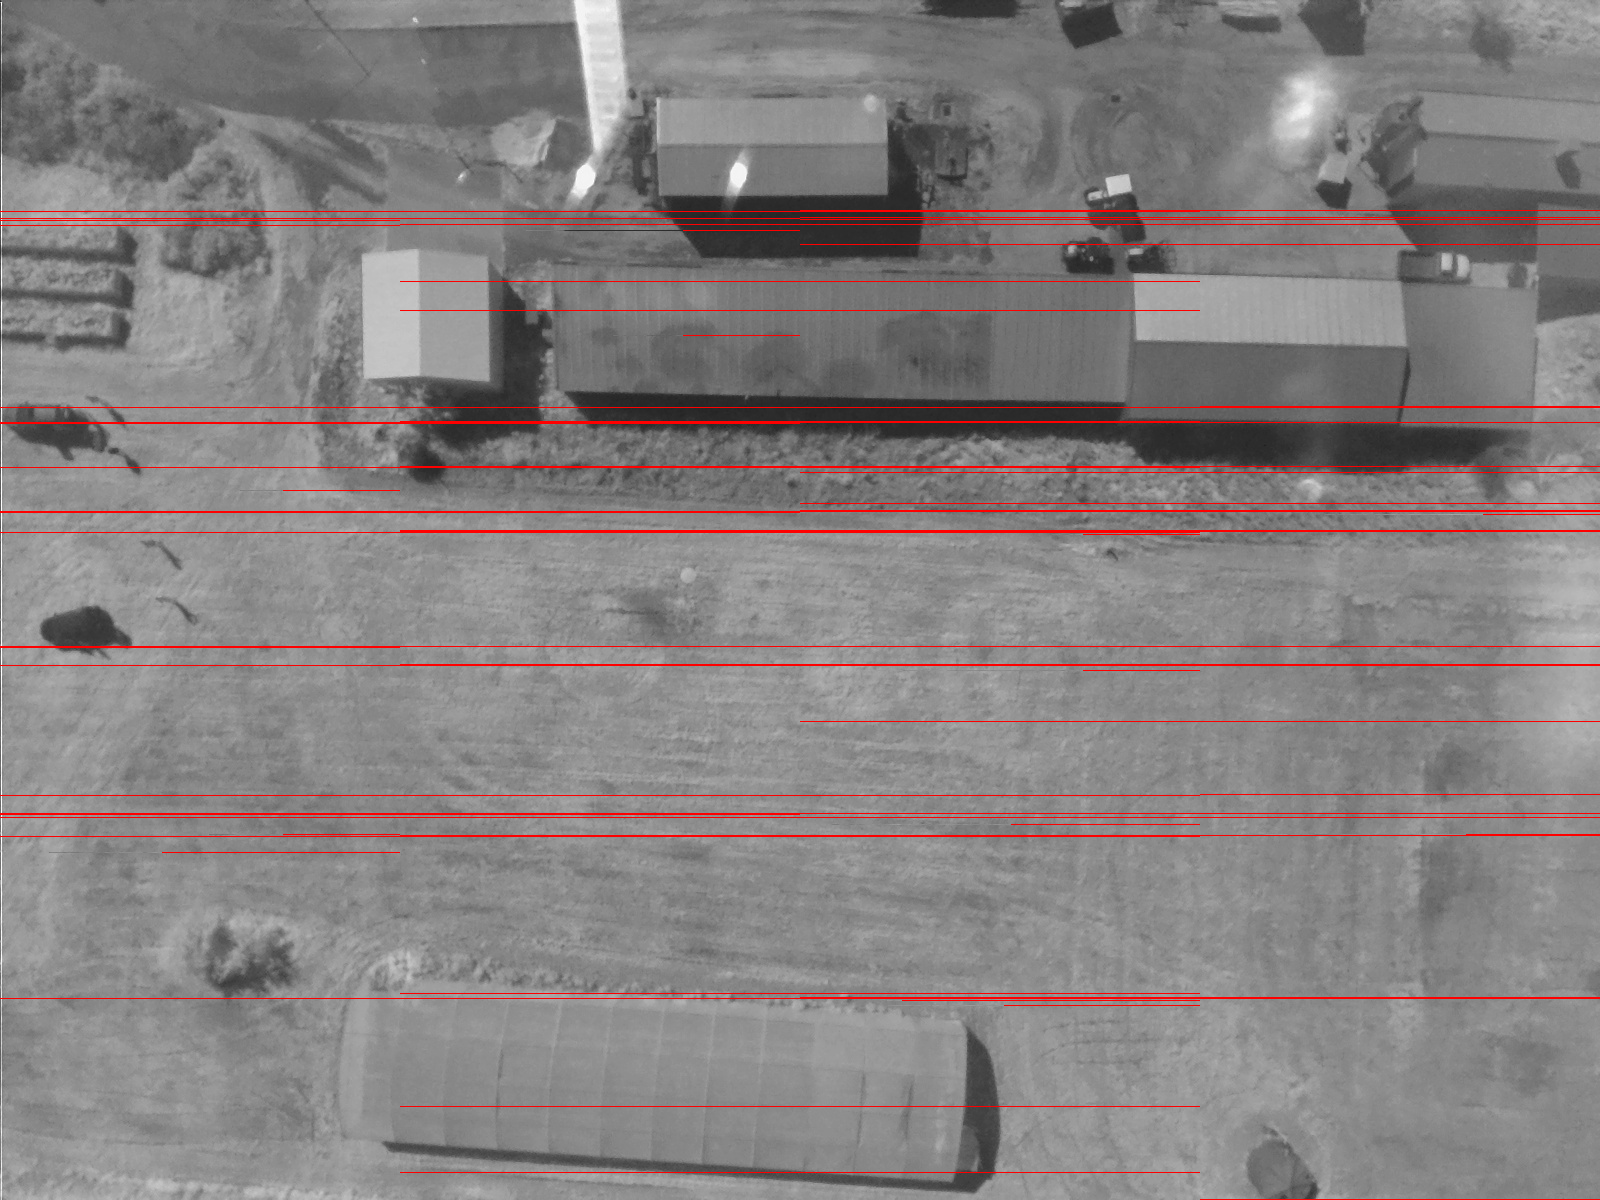
\includegraphics[width=\linewidth]{images/sheds_received.png}
  \caption{Grayscale image of sheds taken at \SI{120}{\metre} AGL. The red pixels are dropped bytes.}
  \label{fig:sheds-received}
\end{figure}

The second \SI{120}{\metre} flight captured another image near roads on the edge of the property, as shown in figure \ref{fig:road-received}. Figure \ref{fig:live-image-reception} shows the ground station during an image download.

\begin{figure}[H]
  \centering
  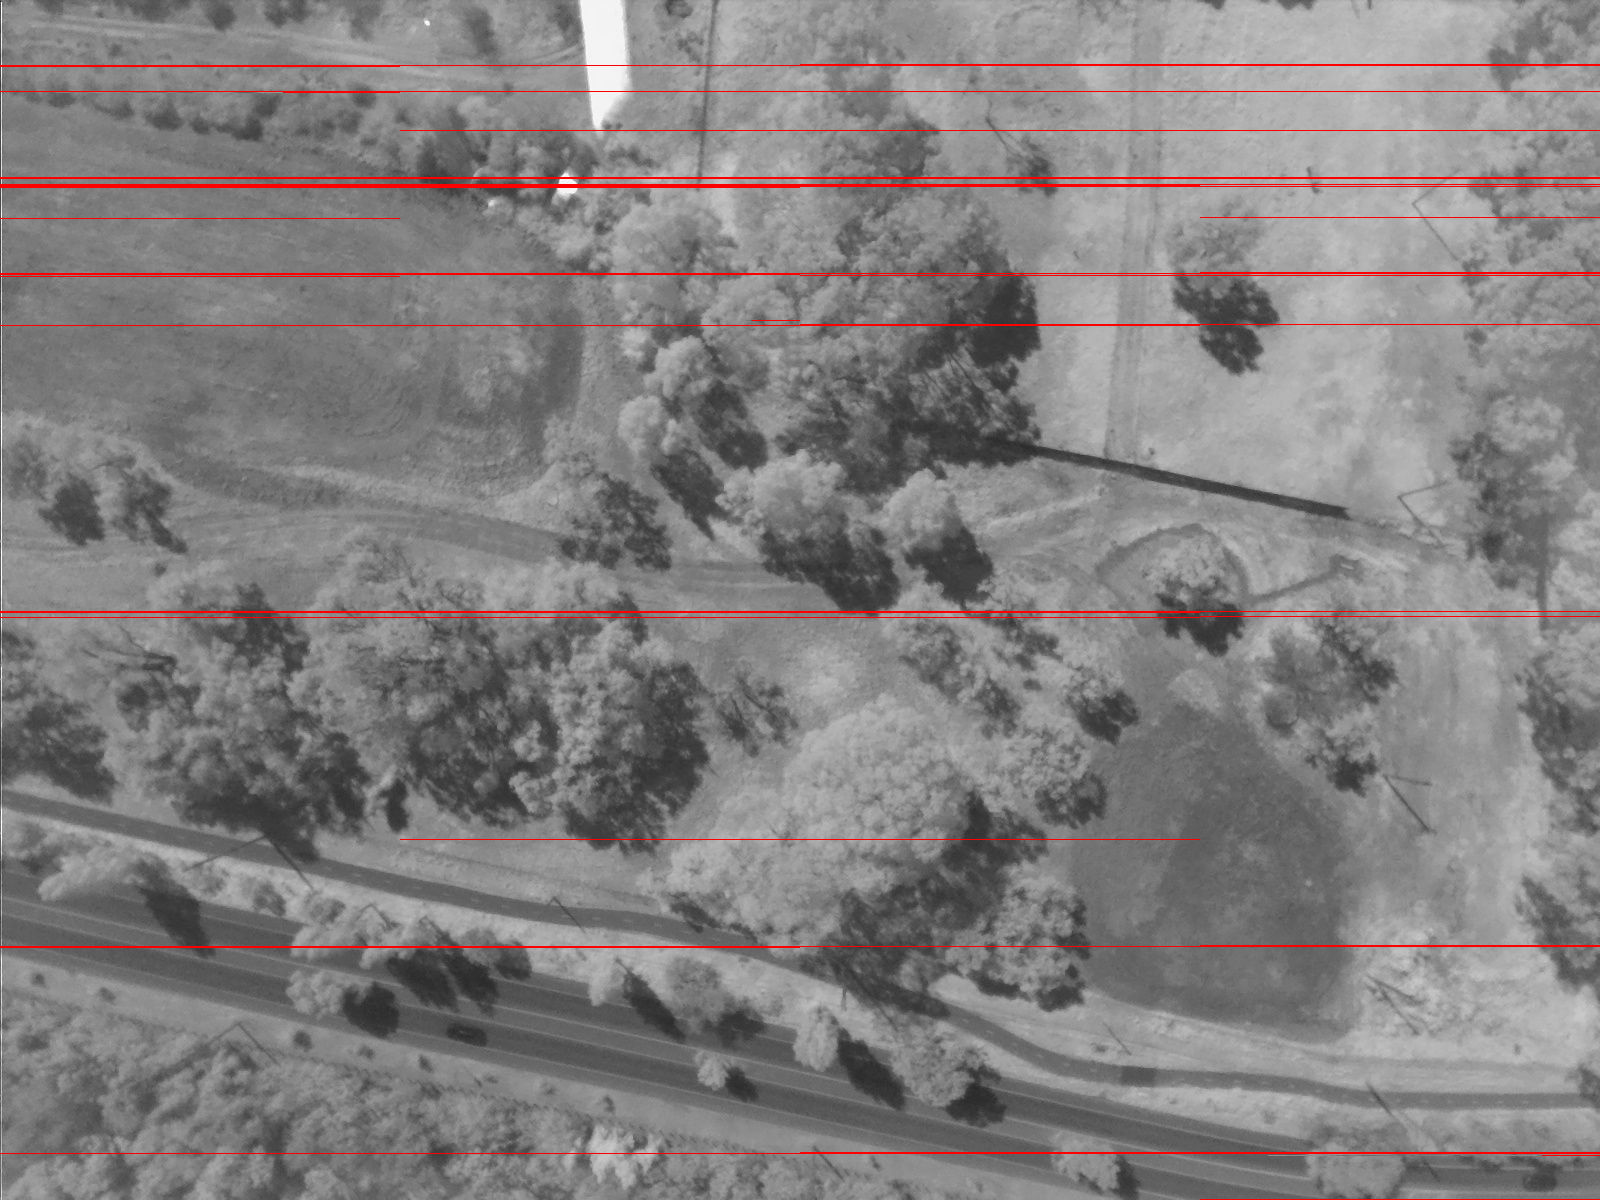
\includegraphics[width=\linewidth]{images/road_received.png}
  \caption{Grayscale image of trees and roads from \SI{120}{\metre} AGL. The red pixels are dropped bytes.}
  \label{fig:road-received}
\end{figure}

\begin{figure}[H]
  \centering
  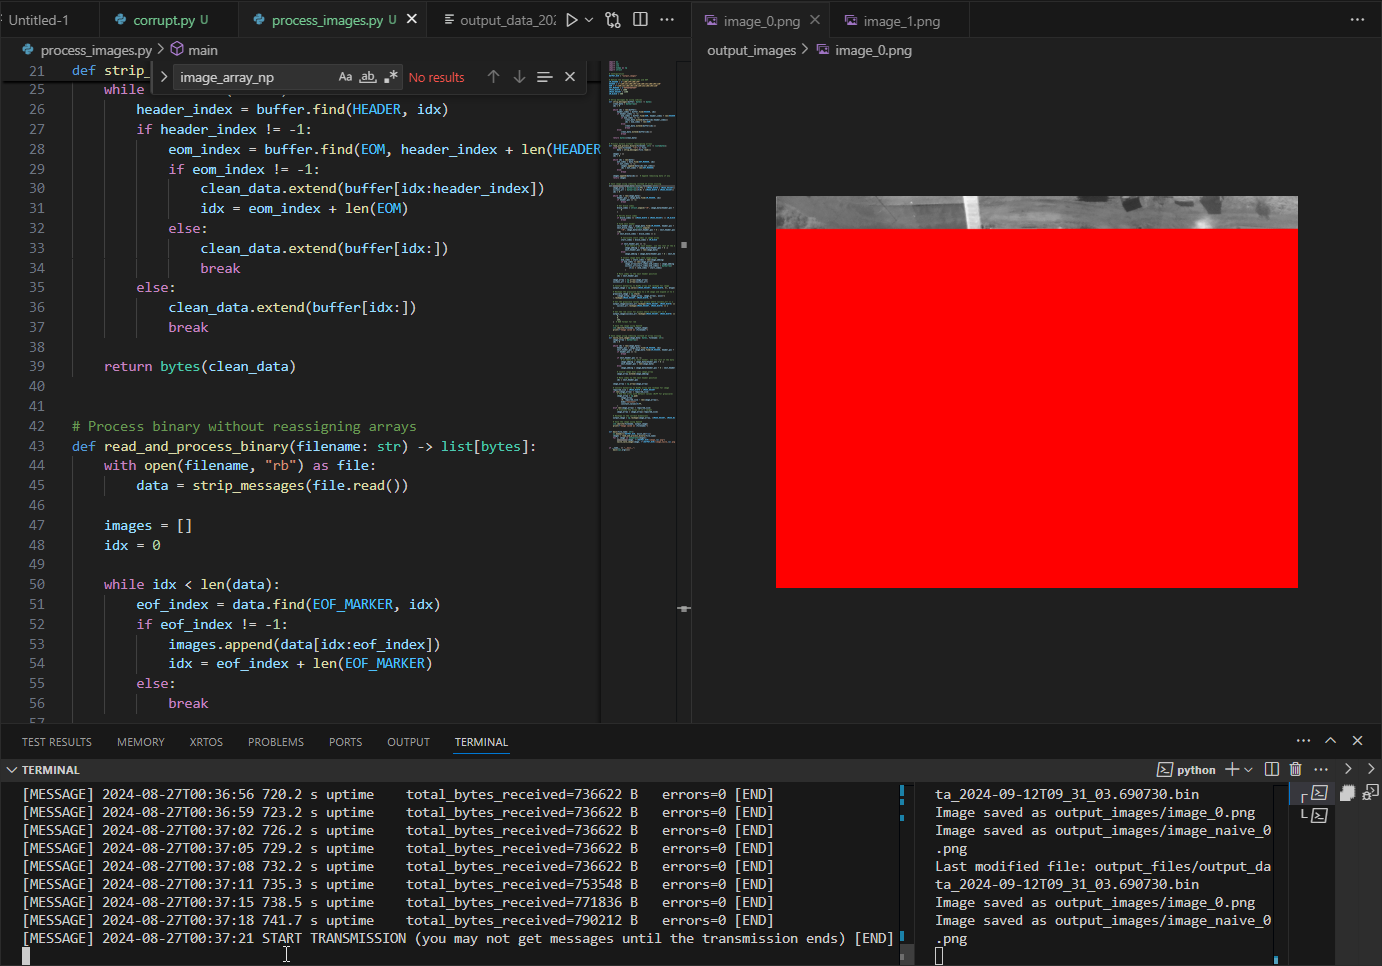
\includegraphics[width=\linewidth]{images/3rd_drone_test_live_reception.png}
  \caption{Screen capture of the ground station during live image download from the CubeSat. The terminal shows the periodic uptime messages which were sent to indicate that the system was online while the camera was capturing an image. A local Python script reassembles the image from the download stream. Red pixels have yet to be downloaded at this point.}
  \label{fig:live-image-reception}
\end{figure}

At this distance, less than 3\% of the image data was not downloaded as shown in table \ref{tabl:image-lost-stats}. In the current implementation, the error manifests as "strips" of lost image pixels since the image is transmitted sequentially.

\begin{table}[H]
  \centering
  \begin{tabular}{|c|c|c|}
    \hline
    \textbf{Image} & \textbf{Lost bytes} & \textbf{Byte error rate} \\\hline
    Sheds          & 45474               & 2.4\%                    \\\hline
    Roads          & 31824               & 1.7\%                    \\\hline
    \textbf{Mean}  & 38649               & 2.0\%                    \\\hline
  \end{tabular}
  \caption{Lost bytes statistics for an image with 1920000 pixels.}
  \label{tabl:image-lost-stats}
\end{table}

\subsection{Discussion}

The first two drone tests were only partial successes but were useful in validating parts of the final DAQ such as the EPS and downlink. However, in the future it would be useful to perform less drone tests since the outcomes of the first two tests could have been achieved through ground testing.

The results of the final drone test were a success, showing the recovery of an image of acceptable quality from a drone at a height of \SI{120}{\metre}. As shown in figure \ref{fig:road-received} and \ref{fig:sheds-received}, the errors are mainly burst errors rather than single byte errors, since an error manifests as multiple sequential bytes being lost. Due to time constraints, it was only possible to implement the blocking image protocol. This protocol is very limited and does not feature state of the art forward error correction (FEC) techniques such as LDPC, turbo codes and BCH \cite{10224067}. These coding schemes are used as part of standard satellite protocols including DVB-S2 and CCSDS file delivery protocol \cite{10224067}. An interleaver changes the order of bits to more evenly distribute burst errors over a bit stream, which allows LDPC and FEC codes to handle burst errors \cite{sonali2021capacity}. Another novel technique would be to use generative adversarial networks on the received image \cite{10131946}, since burst errors result in similar banding errors which are caused by faulty satellite image sensors. The use of FEC would allow compression algorithms to be used, since compressed data is more sensitive to errors. JPEG-LS and CCSDS 123.0-B-2 are image compression algorithms used on imaging satellites \cite{9352211}.

The state of the art for CubeSat testing does not consider a drone test as part of the typical qualification campaign, however this successful result shows that a drone test is a useful test especially for imaging satellites. Typical CubeSat testing campaigns use ground services to emulate supporting equipment available on the launch vehicle, however for the drone test this was not possible due to the limited mass able to be carried. Designing the DAQ as a launch vehicle emulation platform is a useful improvement over the state of the art since it can be used in drone and rocket tests where the launch services need to be emulated, but large equipment is not able to be used.

\section{Temperature Testing}
\subsection{High-Temperature Test}
The high-temperature was performed as described in \secref{sec:htemp-test-framework}. Thermocouples were used to monitor the temperature of the fibreglass panels on the CubeSat frame, which was \SI{80(2)}{\degreeCelsius} at steady-state. Since the tests were not performed at a specialised facility with \liion battery firefighting equipment, the \liion batteries were not used. A DC power supply was used to substitute the batteries, and was set to \SI{3.7}{\volt} DC to emulate the average battery voltage.

The DAQ transmitted picture data from room temperature until \SI{72}{\degreeCelsius}, at which point the camera system failed, and no images were captured. However, the DAQ was still functional to the \SI{80}{\degreeCelsius} target temperature as periodic uptime messages were sent.

\begin{figure}[H]
  \centering
  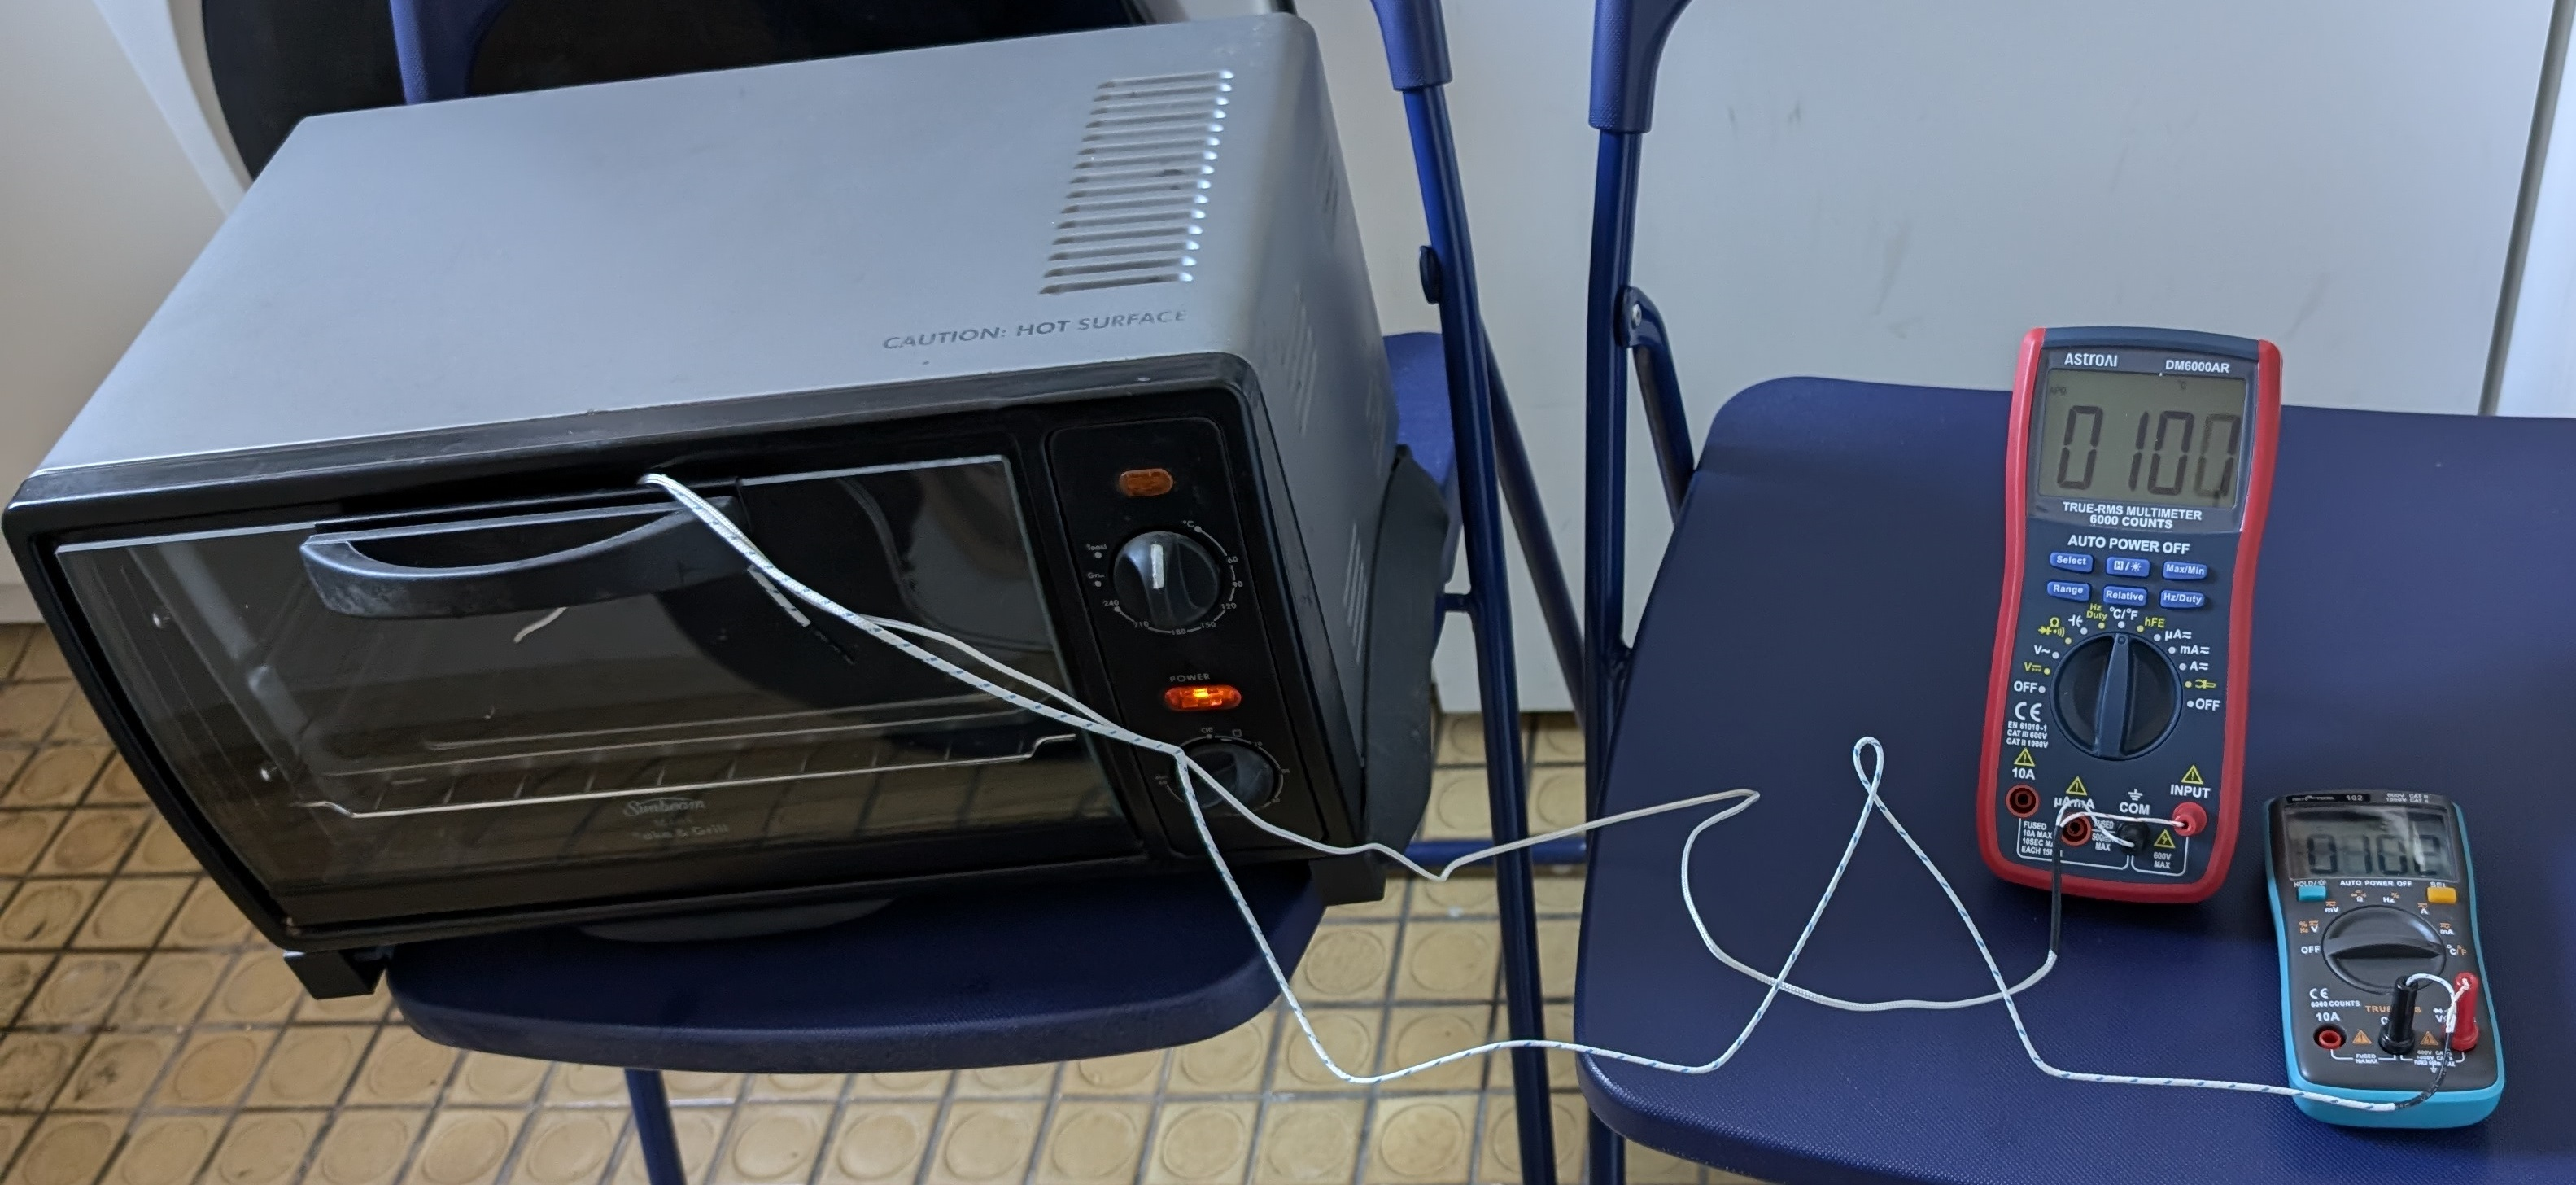
\includegraphics[width=0.75\textwidth]{images/oven_test.jpg}
  \caption{High-temperature testing setup}
  \label{fig:temperature-testing-oven}
\end{figure}

\subsection{Low-Temperature Test}
The low-temperature test was performed as described in \secref{sec:ltemp-test-framework} on \DTMdate{2024-9-12} using a consumer fridge. A thermocouple was placed on the ground plane of the GPS receiver. After \SI{2}{\hour}, the batteries were clipped into the holder and the system was powered for half an hour. After the test the system was turned off and thawed while in the nitrogen bag, to prevent condensation.

The minimum temperature reached in the test was \SI{0}{\degreeCelsius}, which was short of the \SI{-20}{\degreeCelsius} required for qualification. When powered on, the DAQ sent messages indicating the system was online and waiting for picture data from the camera payload. This picture data was not received from the camera payload. It was concluded after test that a USB switch on the camera payload was not rated for temperatures below \SI{0}{\degreeCelsius}, resulting in no image data being saved on the camera payload. Following the test, the device was thawed and rebooted successfully. This indicates that the DAQ, excluding the communication link since this was not tested due to the camera issue, was functional to \SI{0}{\degreeCelsius}.

\begin{figure}[H]
  \centering
  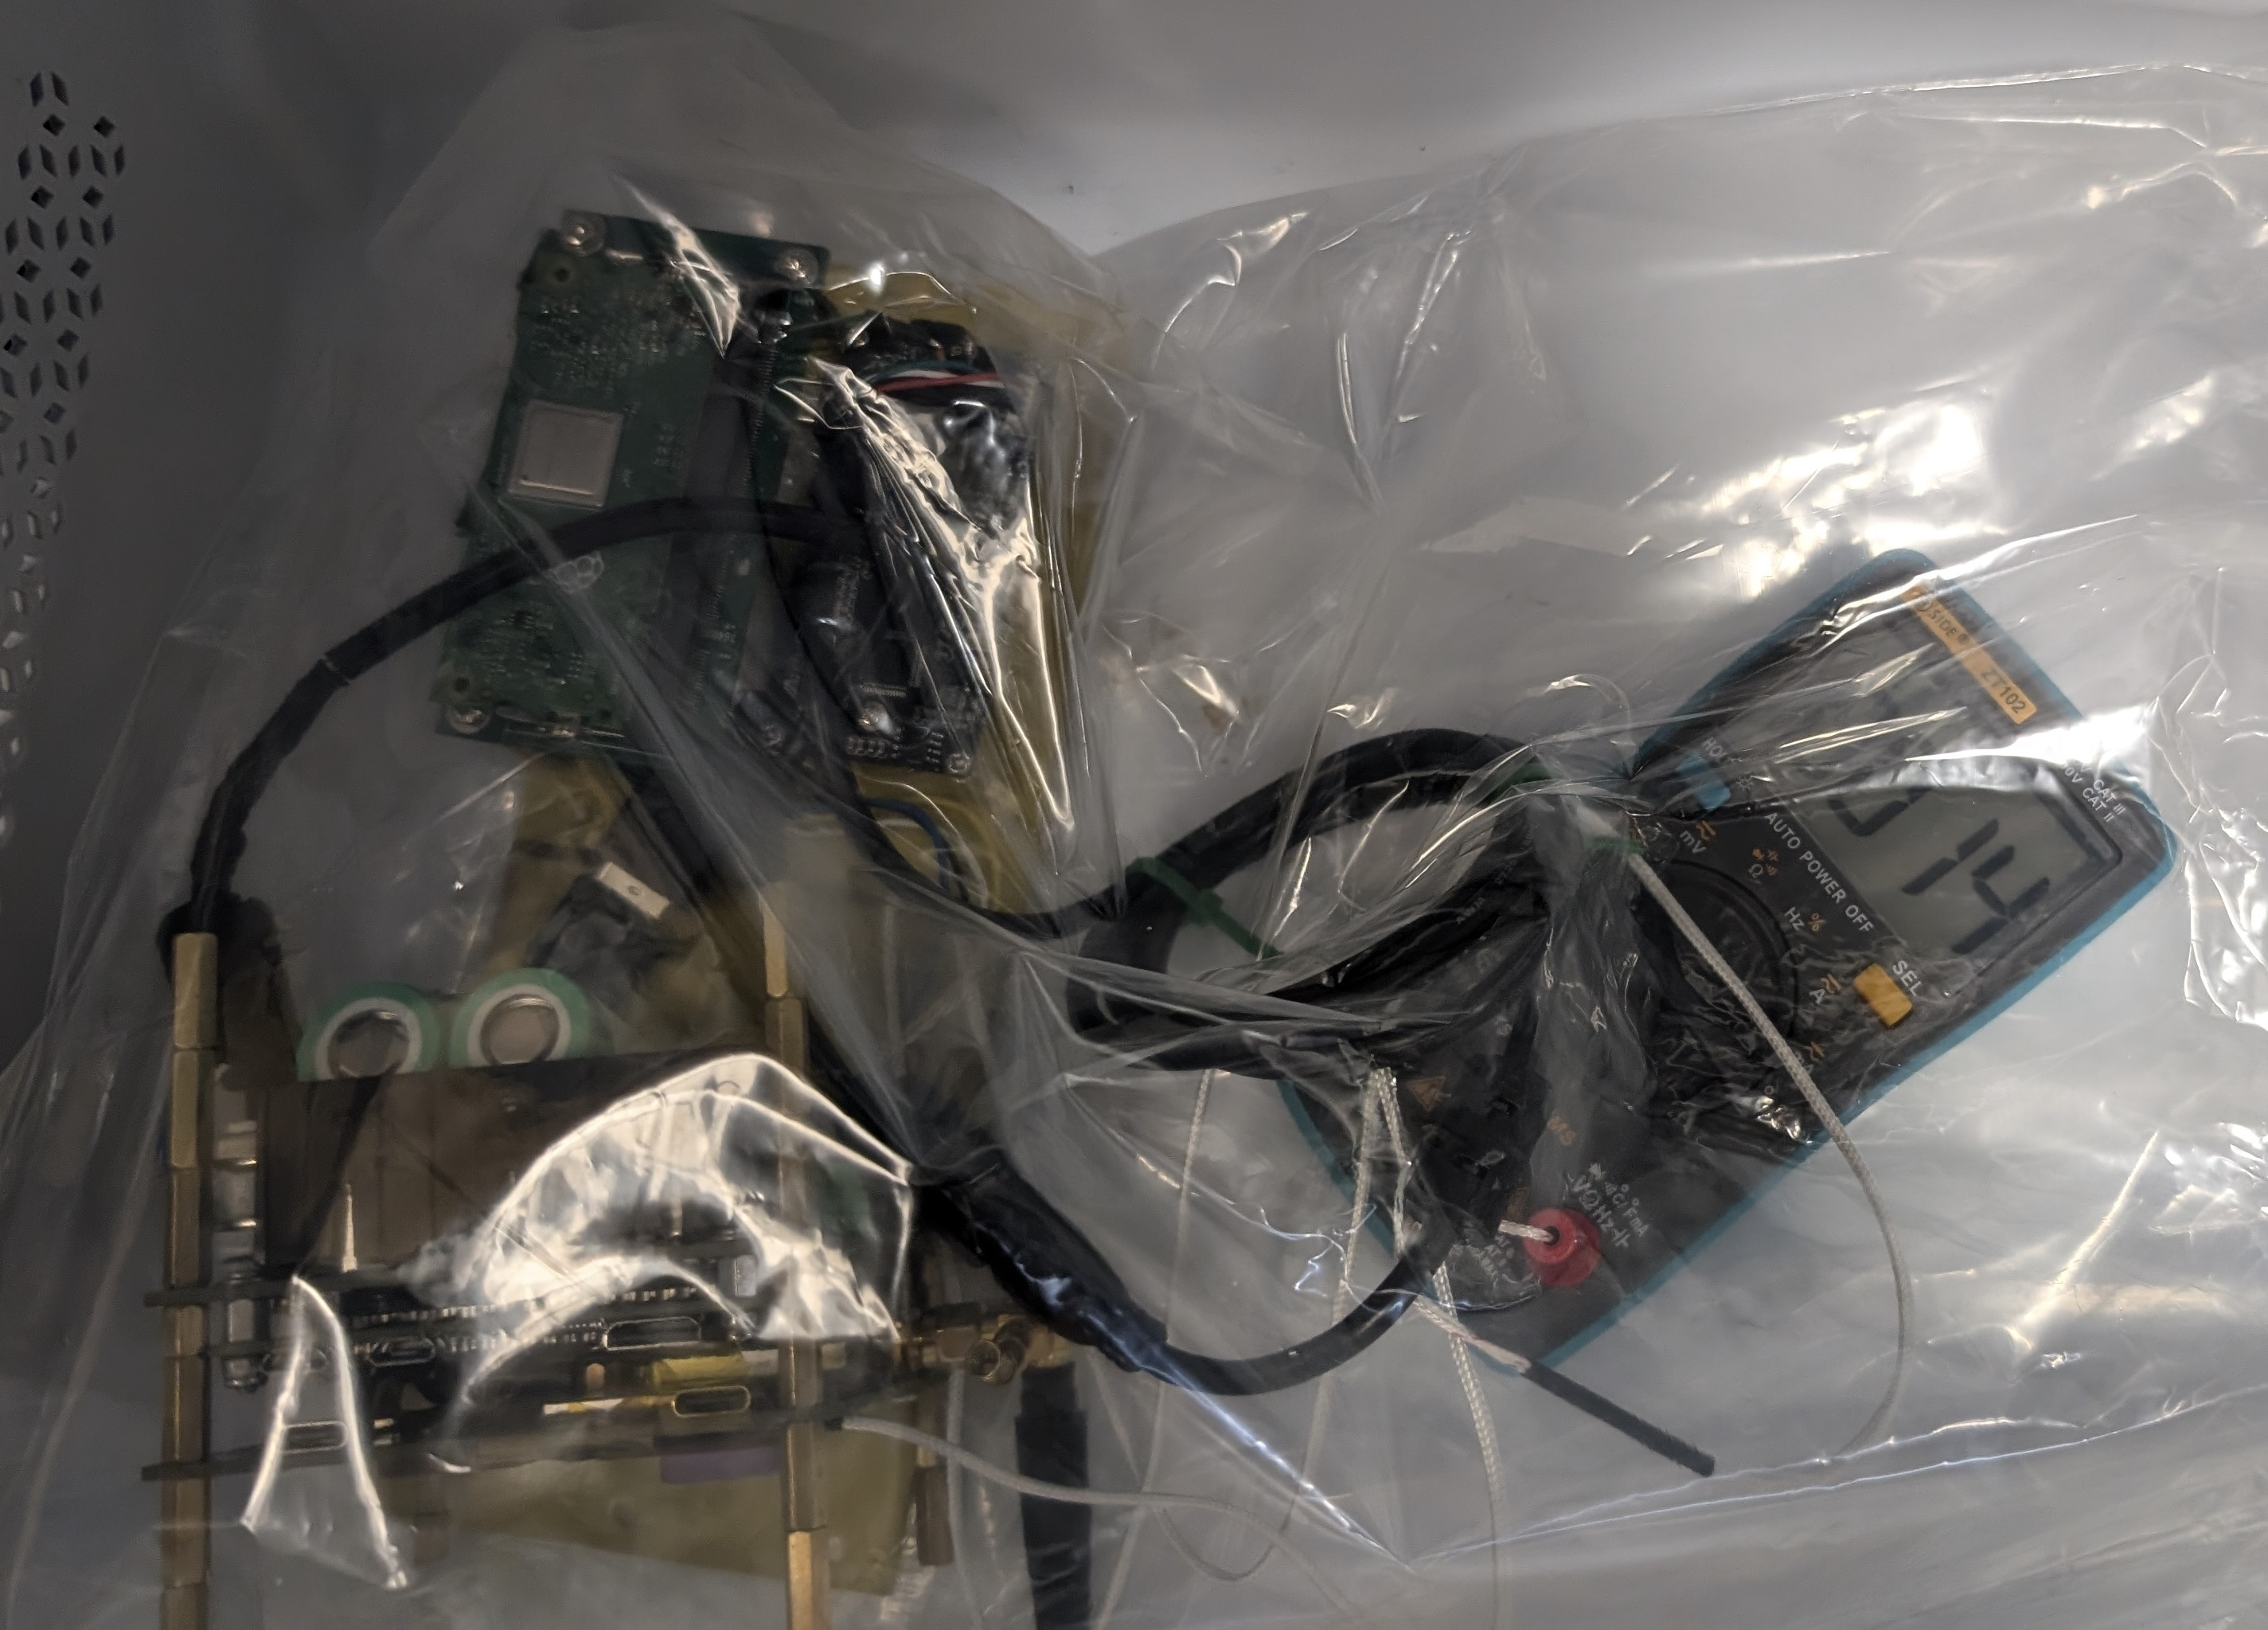
\includegraphics[width=0.75\textwidth]{images/fridge_test.jpg}
  \caption{Low-temperature testing setup}
  \label{fig:temperature-testing-fridge}
\end{figure}

\subsection{Discussion}

These two temperature tests demonstrates that the DAQ can operate from \SIrange{0}{80}{\degreeCelsius} at atmospheric pressure. One of the major goals is to compare the vibration environment on a HPR launch to shaker table and the final space launch, which requires part of this system to be adapted for launch conditions and to be stable in orbit.

While these results were useful as a preliminary measure, it does not show that the DAQ is suitable for a space launch since:
\begin{itemize}
  \item The lowest temperature reached was \SI{0}{\degreeCelsius}, while the qualification target is \SI{-20}{\degreeCelsius} for the cold testing,
  \item The tests were performed at atmospheric pressure, meaning there was convection which would more effectively remove heat from hotspots compared to in a vacuum where only radiative heat transfer is present. It is possible that in a vacuum a hotspot, such as the processor of the Raspberry Pi, could heat up faster than heat can be radiated which could cause loss of performance or device failure.
\end{itemize}

Thermal vacuum testing would be required to qualify the DAQ for space operations.

\section{High-Power Rocket Test Flight}

\textit{UNO} launched with the CubeSat on board on \DTMdate{2024-09-22} at \DTMdisplaytime{12}{52}. The launch and recovery was successful and the DAQ did capture accelerometer data and periodically broadcast uptime messages to the ground station. However, an issue is that the camera payload appears to have booted in an invalid state, resulting in no image being captured or transmitted. An LED on the camera payload was found to be constantly on, which indicates power that is being received, however this LED is only meant to be monetarily on at the beginning of an image capture.

Good acceleration data was captured from the LSM6DSOX accelerometer as shown in figure \ref{fig:flight-16g-time-domain}, however the ADXL375 accelerometer did not produce good data therefore its data was not used in the final analysis. As shown in figure \ref{fig:flight-200g-time-domain}, the data from the ADXL375 is not correlated with any major flight events and is highly noisy. Due to time limitations the cause of the bad data has not been determined.

\begin{figure}[H]
  \centering
  \includesvg[width=\linewidth]{images/flight_acceleration_16g.svg}
  \caption{Time domain flight data from LSM6DSOX accelerometer.}
  \label{fig:flight-16g-time-domain}
\end{figure}

\begin{figure}[H]
  \centering
  \includesvg[width=\linewidth]{images/flight_acceleration_200g.svg}
  \caption{Noisy time domain flight data from ADXL375 accelerometer.}
  \label{fig:flight-200g-time-domain}
\end{figure}

\subsection{Discussion}

The issues with the camera were not simple to debug, since they worked during ground testing before the flight but refused to during and after the flight. This result indicates a need at the very minimum a dual redundant power supply in an OR-ing configuration, where both supplies are active at the same time and if one supply fails, the other automatically powers the payload due to an OR-ing ideal diode. The reliability of the POEM satellite bus is achieved through redundancy, therefore the emulation platform should ideally have some form of redundancy. This was removed from the scope of the final design iteration due to time and budget constraints, but clearly more effort should have been focused on it.

It is speculated in post flight discussion that the camera failure was caused by a race condition in the startup of the camera and Raspberry Pi on the camera payload's side. The payload should have its own watchdog to issues from causing complete failure, especially on the final design launched on POEM, however to be an effective testing platform the DAQ should have a watchdog feature which restarts the camera payload if it does not respond, since this test could have been used to test other parts of the camera system had the startup issue not occurred.

\section{Shaker Table}

The shaker table tests were performed at AVI on the \DTMdate{2024-09-25} using the procedure described in \secref{sec:shaker-table-method}.

\subsection{Random}

The random vibration profile described in table \ref{tabl:random-vibration-profile-iist} was successfully realised on the shaker table, resulting in a response as shown in figure \ref{fig:random-table-resp}. A result from the random vibration test was that it resulted in the DAQ momentarily not responding, then automatically rebooting after 6 minutes.

\begin{figure}[H]
  \centering
  \includesvg[width=\linewidth]{images/random_table.svg}
  \caption{Response of payload from shaker table as recorded by DAQ and IEPE accelerometers.}
  \label{fig:random-table-resp}
\end{figure}

A time-domain sample of the acceleration recorded by the DAQ is shown in figure \ref{fig:noisy-daq}.

\begin{figure}[H]
  \centering
  \includesvg[width=\linewidth]{images/table_acceleration_16g_acc.svg}
  \caption{Noisy accelerometer from the DAQ.}
  \label{fig:noisy-daq}
\end{figure}

\subsection{Shock}

The shock produced the response as shown in figure \ref{fig:shock-table-resp}.

\begin{figure}[H]
  \centering
  \includesvg[width=\linewidth]{images/shock_full.svg}
  \caption{Response of \SI{8}{\milli\second} \SI{50}{\gacc} half-sine shock. The two discontinuities in the shaker table response are a result of the table moving to ensure it stays within the maximum displacement limit.}
  \label{fig:shock-table-resp}
\end{figure}

A result of the shock test is one of the 18650 batteries becoming unmounted from its holder as shown in figure \ref{fig:dislodged-battery}.

\begin{figure}[H]
  \centering
  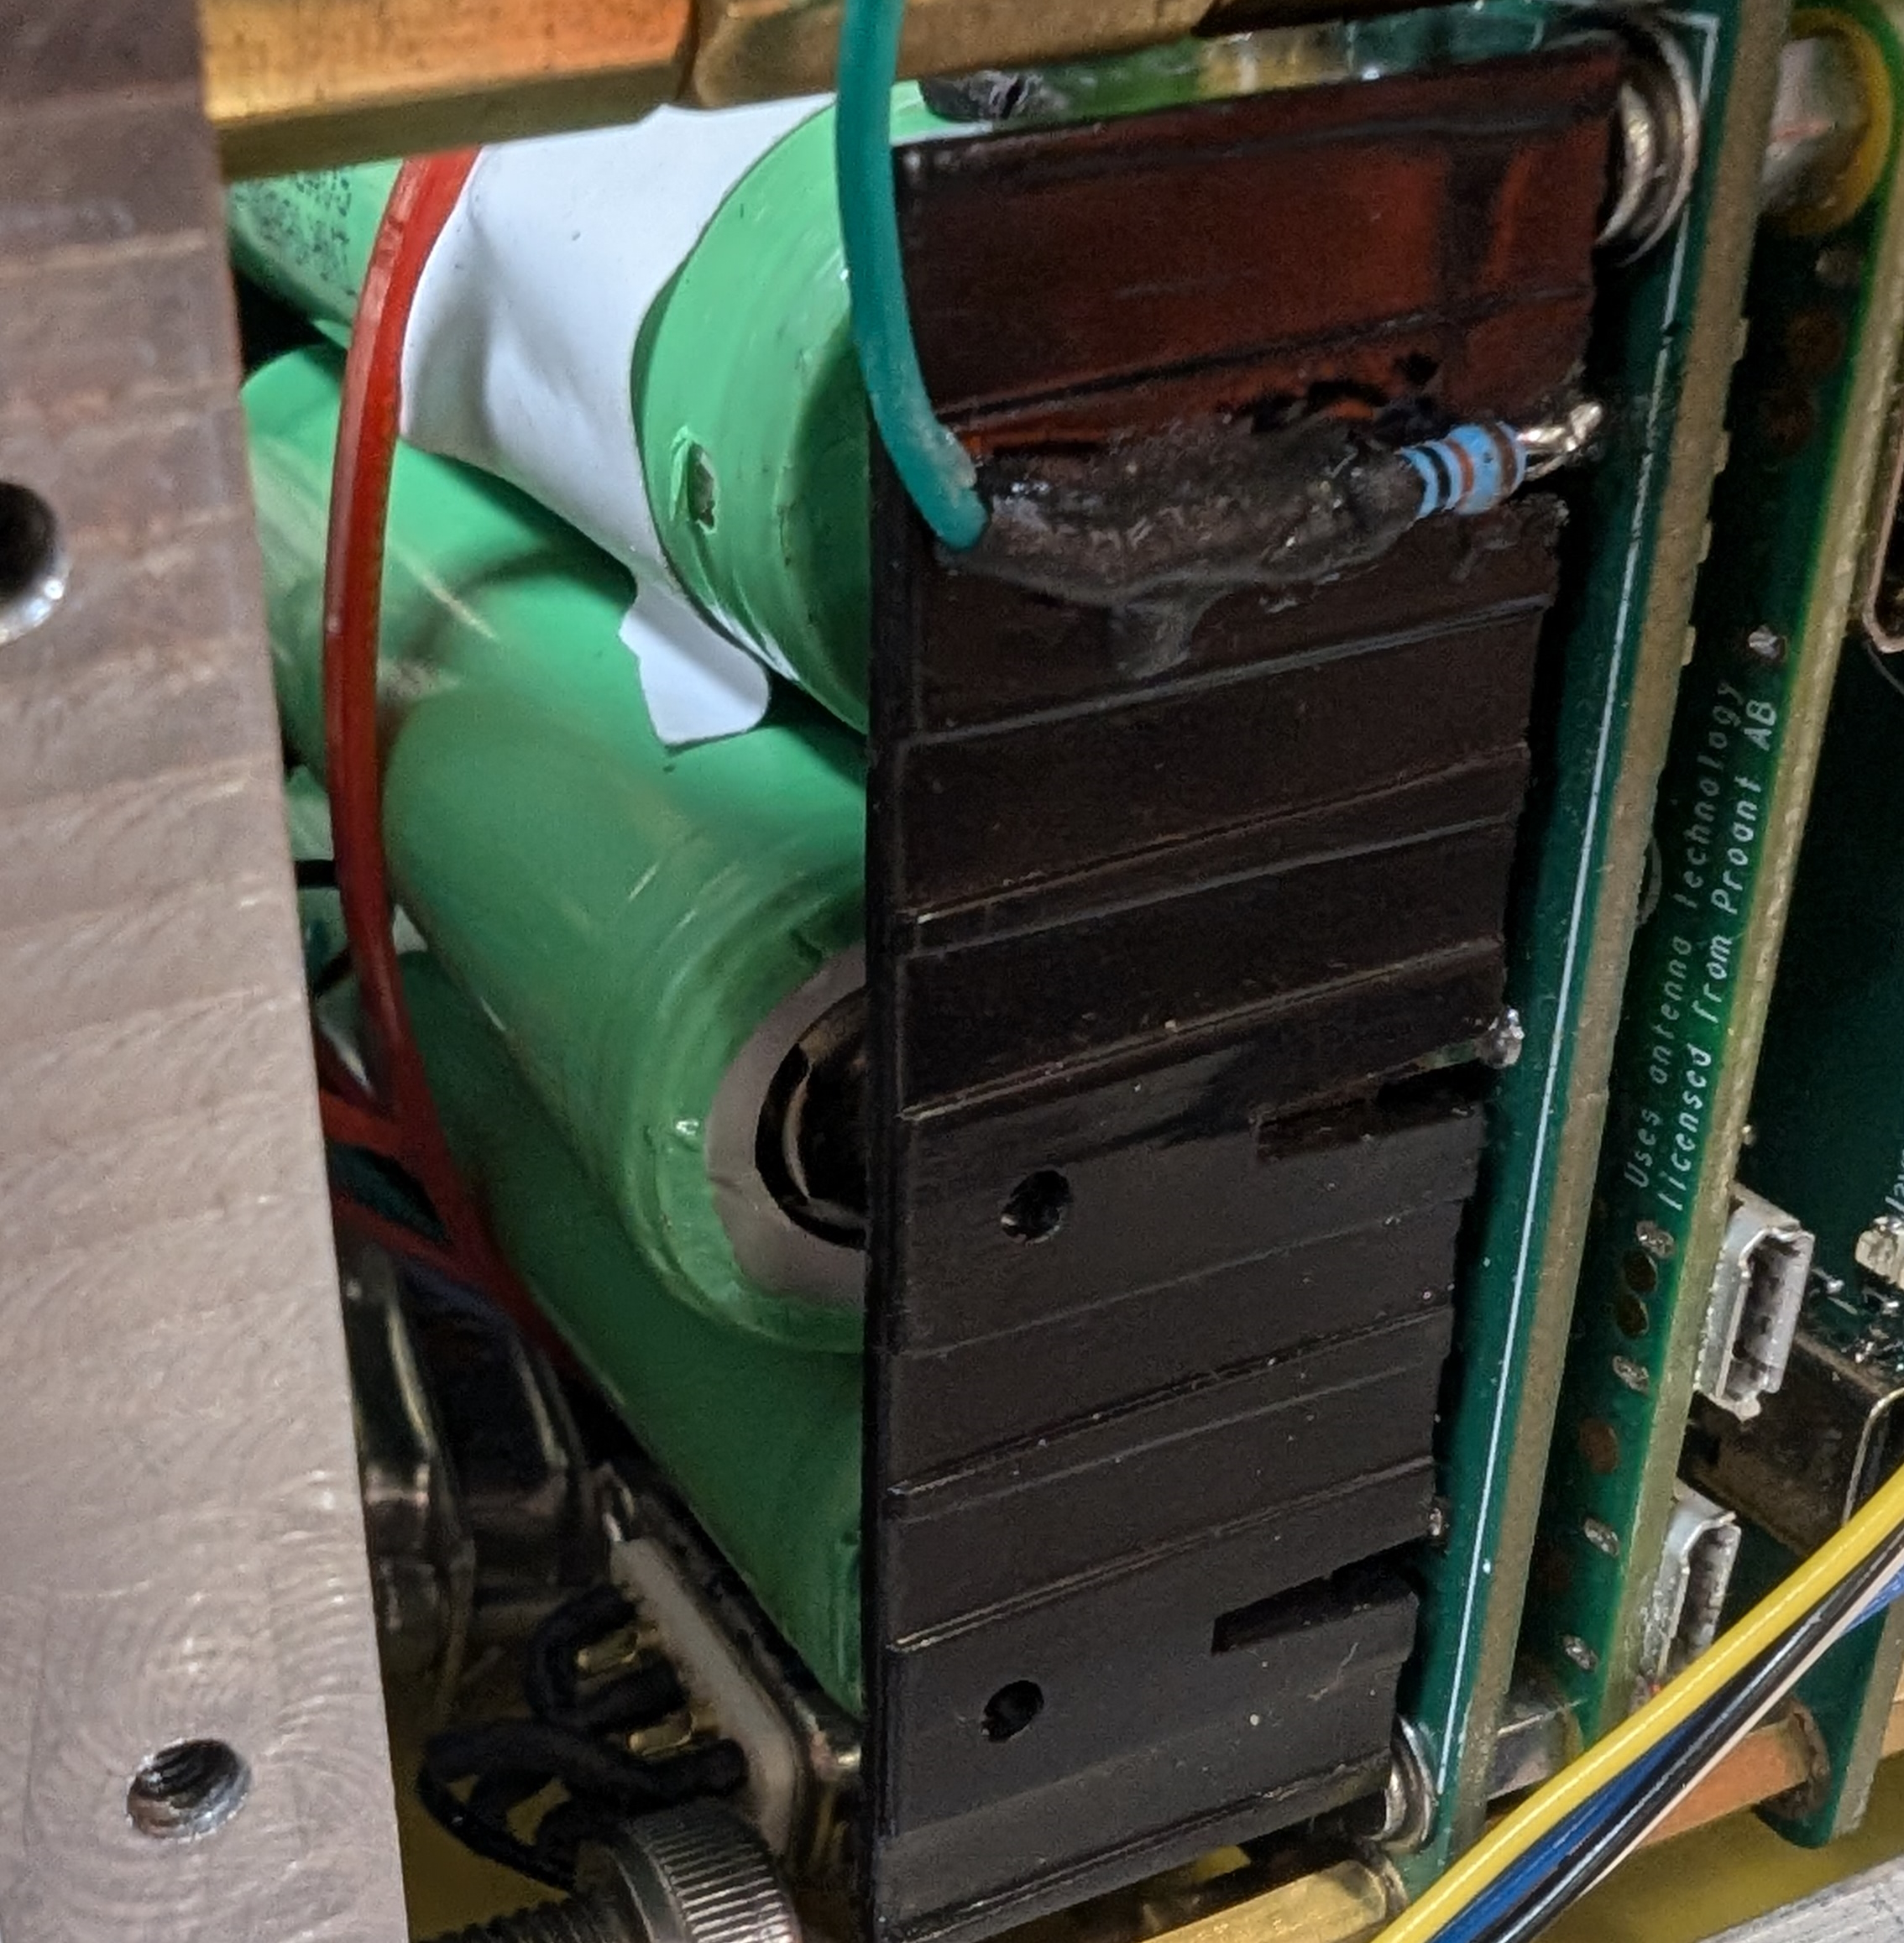
\includegraphics[width=0.7\linewidth]{images/dislodged_battery.jpg}
  \caption{Battery becoming unmounted after shock testing}
  \label{fig:dislodged-battery}
\end{figure}

\subsection{Discussion}

Typically, during shaker table tests on the ground, a CubeSat may be supported with external equipment when it is supported by services provided by the satellite bus. This test shows that the concept is viable as an alternative to external equipment, however the DAQ needs more work to protect it from high vibration environments, including spot welding batteries to the PCB instead of relying on leaf spring terminals. In this particular test, the batteries were not a problem since the two batteries on the sides were held by a cable tie. The reboot of the computer during the random vibration test likely indicates an issue with the quality of wiring harness or some loose element short-circuiting and causing issues.

As shown in figures \ref{fig:random-table-resp} and \ref{fig:noisy-daq}, the MEMS accelerometers did not perform well at recording the response. The recorded PSD is almost white noise and was not useful for analysis. Therefore, for the rest of this analysis the IEPE accelerometer data will be used.

\chapter{Evaluation of HPR Flight as a Qualification Platform}

This chapter will answer if a HPR launch is a viable qualification platform and will evaluate the success of the experiment design.

% The system will be used for the vibration tests on a shaker table, and the rocket test. The data will be recorded as a time series on the OBDH memory. The time series data will be transformed into the frequency domain since existing studies have presented frequency domain plots to present and analyse the response of the system to a test \cite{nasa-pyroshock,nieto2019cubesat}. For the rocket test, the analysis will be split over the several phases of flight - launch, thrust, coast and parachute deployment events, since the forces involved are different in all of these phases.

\section{Random}

The coast and launch phases were compared to the random vibration shaker table test through a PSD, the results are shown in figure \ref{fig:random-psd-result}.

\begin{figure}[H]
  \centering
  \includesvg[width=\linewidth]{images/random.svg}
  \caption{Comparison of shaker table and HPR responses. Shaker table response was captured using IEPE accelerometers, the HPR responses were captured using DAQ accelerometers.}
  \label{fig:random-psd-result}
\end{figure}

\section{Shock}

The half-sine shock test on the shaker table was compared to one parachute deployment event, where a pyrotechnic shock occurred. The two shock responses are shown in figure \ref{fig:shock-resp-result}.

\begin{figure}[H]
  \centering
  \includesvg[width=\linewidth]{images/shock.svg}
  \caption{Shock response of pyroshock and half-sine profile. The two discontinuities in the shaker table response are a result of the table moving to ensure it stays within the maximum displacement limit.}
  \label{fig:shock-resp-result}
\end{figure}

The SRS was created using the time-domain data in figure \ref{fig:shock-resp-result}, using a damping factor of $Q=10$. As shown in \ref{fig:srs}, the SRS of the rocket consistently has a lower peak acceleration than the SRS of the half-sine shock for all frequencies between \SIrange{10}{10000}{\hertz}

\begin{figure}[H]
  \centering
  \includesvg[width=\linewidth]{images/srs.svg}
  \caption{Shock response of pyroshock and half-sine shock.}
  \label{fig:srs}
\end{figure}

\section{Discussion}

The experiment was successful in showing that HPR was not a suitable vibration qualification procedure for a CubeSat using a K1100T motor. The pyroshock events generated on the HPR flight had lower peak accelerations (Consistently 1 order of magnitude less) across the spectrum compared to the qualification response from the IIST profile. The random vibration response from both the launch and coast phases were consistently below both the shaker table response, and the qualification profile.

This experiment design was adequate for this case, since the goal was to answer a simple yes or no question about if HPRs are suitable for qualification. However, future tests may require a more comprehensive comparison since it is possible that with a different HPR motor or components that there are portions of the test which meet the qualification level. This type of comparison may include determining what frequencies the HPR test are effective at comparing, or using coherence to compare the PSDs numerically.

% TODO: 10%
\chapter{Conclusions and Future Work}

\section{Future Work}

While this design was successful in showing the inadequacy of HPR launches for qualification, another question is whether current shaker table tests are over-qualifying CubeSats. A useful extension of this work would be to put the DAQ on the PSLV POEM and measure the real vibration environment during launch. This would allow direct comparison between both HPR and shaker table testing to the real conditions.

However, to launch the DAQ on POEM a future design would need to be created which would incorporate all the learnings from this design including:

\begin{itemize}
  \item Machine a heatsink to connect all chips on the Pi Zero module to the chassis or heatsink to ensure better thermal performance in vacuum \cite{guertin2022raspberry}.
  \item Batteries should be spot welded to tabs that are soldered fixed to the PCB to make pack resistant to random vibration rather than using the current leaf springs.
  \item Use IEPE accelerometers and integrate an analog front end for the accelerometers on the DAQ instead of using MEMS accelerometers, since this work has shown MEMS accelerometers to underperform for vibration analysis.
  \item Investigate the use of a real-time operating system instead of Raspbian.
  \item Implement a watchdog to increase reliability.
\end{itemize}

To qualify the future design, the testing campaign would need to repeated. While the fridge and oven tests were found to be useful preliminary tests for partially qualifying the temperature range of components, a final test should be performed using a thermal vacuum chamber.

Other design improvements that would be useful for future HPR launches include:
\begin{itemize}
  \item Use of error correcting codes such as LDPC codes with interleaving and compression to provide higher downlink speeds and reduced error rates, which would be good since drone and HPR tests are relatively short \cite{sonali2021capacity}.
  \item Implement a watchdog to reset the payload-under-test if it fails, to get more value out of the tests.
  \item Use two independent power supplies in an OR-ing configuration to implement power supply redundancy.
\end{itemize}

This work was limited by motor sourcing issues, therefore the experiment should be repeated for more significant M impulse class motors, which have ten times the total impulse and may be able to provide the random vibration environment seen in shaker table testing.

The experiment developed in this work could only answer if HPR launches were useful for qualification or not, but it could not say to what degree they differ from shaker table testing (and potentially the real POEM launch). An experiment which quantifies the difference will have to be developed in the future.

\section{Conclusions}

This work developed a novel data acquisition and emulation platform for the POEM intended to be used in tests on a HPR or drone qualification platform and an experiment to evaluate the usefulness of HPR launches as a CubeSat qualification method. The DAQ was used to evaluate whether the HPR is a viable alternative to shaker tables as a vibration qualification platform. The vibration profile from the HPR launch, captured using the DAQ, was compared to the profile from the shaker table test. While the shaker table performed at, or above, the IIST recommended qualification level for POEM for all tests except the quasi-static acceleration test, the HPR launch produced a vibration profile that was consistently below the qualification level, therefore the conclusion is that HPR launches using a K1100T motor or lower are not a good vibration qualification platform. While the motor may be able to be changed in future flights to produce a stronger random vibration spectrum that may meet the qualification level, it is unlikely that HPR launches will ever be a substitute for shock testing since a larger launch does not use significantly larger black powder charges.

Since HPR testing was a novel qualification method, there were few designs on how a CubeSat should be supported during the launch. Traditionally, a satellite bus would be emulated using heavy ground equipment such as power supplies and computers. This work developed a novel test platform which emulated the final satellite bus the CubeSat will use, at specifications required for HPR flight. While HPR launches below a K1100T motor are not an ideal qualification platform, the drone tests were especially useful for qualifying the camera hardware. This emulation platform has a future in drone testing of CubeSats with optical payloads, since the mass restrictions of the HPR launch also apply to the drone.

\newpage

\section{Appendix}

\subsection{Code}

Code and material from this research is available at the following git repositories:

\begin{itemize}
  \item \url{https://git.petertanner.dev/peter/Honours-DAQ-software}
  \item \url{https://git.petertanner.dev/peter/Honours-DAQ-PCB}
  \item \url{https://git.petertanner.dev/peter/Honours-Data-Processing}
  \item \url{https://git.petertanner.dev/peter/Honours-Thesis}
\end{itemize}

\subsection{References}

\printbibliography[heading=none]

\end{document}
